% !TeX root = main
\documentclass[titlepage,  ngerman]{article}
\usepackage[nottoc,numbib]{tocbibind}
\usepackage[utf8]{inputenc}
\usepackage[german]{babel}
\usepackage{graphicx} 
\usepackage{amsmath, amssymb}
\usepackage[section]{placeins}
\usepackage[square,numbers]{natbib}
\bibliographystyle{abbrvnat}
\usepackage{mathtools}
\usepackage{caption}
\usepackage{subcaption}
\usepackage{chngcntr}
\counterwithin{figure}{section}
\counterwithin{equation}{section}
\counterwithin{table}{section}
\usepackage[left=3.50cm, right=3.50cm, top=3.00cm, bottom=3.00cm]{geometry}
\usepackage[normalem]{ulem}
\useunder{\uline}{\ul}{}
\usepackage{rotating}
\renewcommand{\Re}{\operatorname{\mathbb{R}e}}
\renewcommand{\Im}{\operatorname{\mathbb{I}m}}

%\renewcommand{\subsection}{\FloatBarrier\subsection}
%\renewcommand{\subsubsection}{\FloatBarrier\subsubsection}
\usepackage[hidelinks]{hyperref}
\usepackage{cleveref}

%\binoppenalty=\maxdimen
%\relpenalty=\maxdimen

\title{Aufbau und Justage eines Leckstrahlmikroskops zum Nachweis des plasmonischen Spin-Hall-Effektes}
\author{Hanno Christiansen}
\date{März 2021}

\begin{document}
	
	\maketitle
	\tableofcontents
	\newpage
	\listoffigures 
	\newpage
	
	\section{Einführung}
	Ein Leckstrahlmikroskop (engl. \textbf{L}eakage \textbf{R}adiation \textbf{M}icroscope LRM) dient der Beobachtung von Oberflächen-Plasmon-Polaritonen (engl. \textbf{S}urface \textbf{P}lasmon \textbf{P}olariton SPP). Ein SPP ist eine kollektive Ladungsdichteoszillation der freien Elektronen in einem Metall an der Grenzschicht zu einem Dielektrikum. Diese Elektronendichtewelle ist stark an das elektromagnetische Feld des Dielektrikums gebunden und eng an der Grenzschicht lokalisiert. SPP können, wenn sie an sehr dünnen Metallfilmen angeregt werden, unter bestimmten Umständen elektromagnetische Strahlung an einer zweiten Grenzschicht in ein weiteres Dielektrikum abgeben. Diese Strahlung wird als Leckstrahlung bezeichnet und kann im Fernfeld mit einem LRM beobachtet werden. Aus der Leckstrahlung können verschiedene Rückschlüsse auf die Eigenschaften des SPP gezogen werden.\cite{Drezet.2008}
	
	Da die räumliche Ausdehnung von SPP maßgeblich durch die Geometrie ihrer Trägerstruktur und nicht durch die optische Wellenlänge bestimmt wird, ist es möglich, das klassische Beugungslimit zu umgehen. Speziell können SPP auf gezielt hergestellten Strukturen genutzt werden, um auf einer Oberfläche optische Informationen zu transportieren. Außerdem reagieren SPP empfindlich auf die optischen Eigenschaften ihrer Trägerstruktur und können deswegen für Anwendungen in der Sensorik zum Einsatz kommen.\cite{Lin.2013}
	
	SPP können durch unterschiedliche Mechanismen erzeugt werden. Beispielsweise können SPP durch elektromagnetische Strahlung (EM-Strahlung) an einem Defekt auf einer Goldoberfläche angeregt werden. Der plasmonische Spin-Hall-Effekt (engl. \textbf{P}lasmonic \textbf{S}pin \textbf{H}all \textbf{E}ffect PSHE) tritt auf, wenn diese anregende EM-Strahlung elliptisch polarisiert ist und den Defekt unter schrägem Einfall trifft. Durch Nahfeldinterferenz an dem Defekt findet die SPP-Anregung dann gerichtet statt. Die effektivste Anregungsrichtung hängt hierbei von dem Drehsinn der elliptischen Polarisation ab. Dieser Effekt könnte dafür genutzt werden, die Propagationsrichtung von SPP in plasmonischen Bauteilen gezielt zu steuern. Hierdurch wäre es zum Beispiel möglich Informationen durch den Polarisationszustand zu codieren. Durch die Polarisationsabhängigkeit des Effektes sind auch Anwendungen in der Sensorik denkbar.\cite{RodriguezFortuno.2013}
	
	Im plasmonische Spin-Hall-Effekt werden also, genau wie bei dem elektronischen Spin-Hall-Effekt, Teilchen abhängig von ihrer Spin-Orientierung in unterschiedliche Richtungen senkrecht zu ihrer ursprünglichen Bewegungsrichtung abgelenkt. Bei der plasmonischen Variante sind diese Teilchen Photonen bzw. Plasmonen und bei der elektronischen Variante sind es Elektronen. \cite{Inoue.2005}
	
	Ziel dieser Arbeit ist es, zunächst ein vorhandenes LRM so zu modifizieren, dass eine Beobachtung des PSHE möglich wird. Im nächsten Schritt soll der PSHE dann an einem Defekt in einem Luft-Gold-Glas-System nachgewiesen werden. Im ersten Teil dieser Arbeit werden daher einige Grundlagen der Plasmonik diskutiert, die für ein Verständnis der Leckstrahlmikroskopie notwendig sind. Außerdem wird im ersten Teil auf wichtige Details des PSHE eingegangen. In dem Kapitel \textit{Messung und Methoden} werden das verwendete LRM und die in dieser Arbeit durchgeführten Modifikationen detailliert erläutert. Das Kapitel \textit{Ergebnisse und Diskussion} befasst sich mit der Auswertung und Interpretation der aufgezeichneten Messdaten. Abschließend werden die Ergebnisse kurz zusammengefasst, und es wird ein Ausblick auf zukünftig mögliche Projekte gegeben.
	
	\newpage	
	\section{Theorie}
	\subsection{Oberflächen-Plasmon-Polariton (SPP)}		
	Ein SPP ist das quantisierte Quasiteilchen einer an das elektromagnetische Feld gekoppelten Elektronen-Dichte-Oszillation an einer Grenzschicht zwischen einem Metall und einem Dielektrikum. Durch die spezielle Form dieser Grenzschichtgeometrie ist es möglich, trotz des rein longitudinalen Charakters der Elektronen-Dichte-Oszillation ein elektromagnetisches Feld mit transversalen Komponenten zu erzeugen. Das magnetische Feld eines SPP ist hingegen rein transversal. Daher spricht man auch von einer transversal-magnetischen Mode (TM-Mode). Durch die Existenz dieser transversalen Komponenten ist eine Kopplung zwischen SPP und der rein transversalen elektromagnetischen Strahlung prinzipiell möglich. Die einfachste Geometrie, in der SPP auftreten können, ist ein Zweischichtsystem: Der Halbraum oberhalb der $xy$-Ebene mit $z>0$ sei von einem Dielektrikum mit der Dielektrizitätskonstante $\epsilon_\mathrm{D}$ ausgefüllt. Im Halbraum unterhalb der $xy$-Ebene mit $z<0$ befinde sich ein Metall mit der im allgemeinen komplexen dielektrischen Funktion $\epsilon(\omega)$. An der Grenzschicht zwischen diesen beiden Halbräumen können SPP propagieren. Um nun einige charakteristische Eigenschaften von SPP zu erläutern, wird davon ausgegangen, dass das SPP entlang der $x$-Achse propagiert und entlang der y-Achse homogen ist. So wird das Problem effektiv auf zwei Dimensionen reduziert. Wie in \cite{Maier.2007} gezeigt, lassen sich die elektromagnetischen Felder eines SPP in dieser einfachen Geometrie durch folgende Ausdrücke beschreiben:
	\begin{subequations}
		\label{eq:fields_spp}
		\begin{equation}
			\label{eq:electric_field_spp}
			\vec{E}_n(\vec{r}) = \begin{pmatrix} 1 \\ 0 \\ \pm k_{\mathrm{spp}}/k_{z,n} \end{pmatrix} E_0 \exp\left(i(k_{\mathrm{spp}}x + k_{z, n}|z|-\omega t)\right)	
		\end{equation}
		\begin{equation}
			\label{eq:magnetic_field_spp}
			\vec{H}_n(\vec{r}) = \begin{pmatrix} 0 \\ 1 \\ 0 \end{pmatrix} H_0 \exp\left(i(k_{\mathrm{spp}}x + k_{z, n}|z|-\omega t)\right)
		\end{equation}
	\end{subequations}
	Hierbei ist $\vec{E}_n(\vec{r})$ die elektrische Feldstärke im Medium $n$ am Ort $\vec{r}$, $E_0$ die Amplitude der elektrischen Feldstärke an der Grenzschicht, $\omega$ die Kreisfrequenz der Anregung, $x, z$ Komponenten von $\vec{r}$, $\vec{H}_n(\vec{r})$ die magnetische Feldstärke am Ort $\vec{r}$ im Medium $n$, $H_0$ die Amplitude der magnetischen Feldstärke an der Grenzschicht und $t$ die Zeit. Der komplexe Wellenvektor der Anregung entlang der Grenzfläche ist $k_{\mathrm{spp}}$, während der senkrechte Anteil des Wellenvektors durch $k_{z,n}$ beschrieben wird.
	Der Index $n$ beschreibt hierbei das Material ($\mathrm{M}$ für das Metall, $\mathrm{D}$ für das Dielektrikum). 
	In dem Operator $\pm$ steht das $+$ für das Metall und das $-$ für das Dielektrikum. Der im allgemeinen komplexe Wellenvektor der Anregung $k_{\mathrm{spp}}$ ist in beiden Materialien identisch. Der Realteil $\Re\{k_{\mathrm{spp}}\}$ des komplexen Wellenvektors lässt sich in die Wellenlänge $\lambda_{\mathrm{spp}} = 2\pi/ \Re\{k_{\mathrm{spp}}\} $ des SPP umrechnen. Der Imaginärteil $\Im\{k_{\mathrm{spp}}\}$ beschreibt das Dämpfungsverhalten des SPP entlang der Ausbreitungsrichtung. Der Imaginärteil lässt sich über $L_{\mathrm{spp}} = 1/(2\Im\{k_{\mathrm{spp}}\})$ in eine Propagationslänge umrechnen.  Hierfür gilt: Nachdem das SPP eine Propagationslänge in Ausbreitungsrichtung zurückgelegt hat, sind die ursprünglichen Amplituden des SPP auf $1/\mathrm{e}$ ihres ursprünglichen Betrages abgeklungen. Analog beschreibt $\Im\{k_{z, n}\}$ das exponentielle Abklingen der Anregung senkrecht zur Grenzfläche. Hier lassen sich anlog zur Propagationslänge die Eindringtiefen $\delta_{\mathrm{M,D}}$ definieren. Der quantitative Verlauf des elektrischen Feldes ist für ein rein reelles $k_{\mathrm{spp}}$ und rein imaginäre $k_{z, n}$ in Abb. \ref{fig:electric_field_spp} dargestellt. 
	\begin{figure}[htbp] 
		\centering
		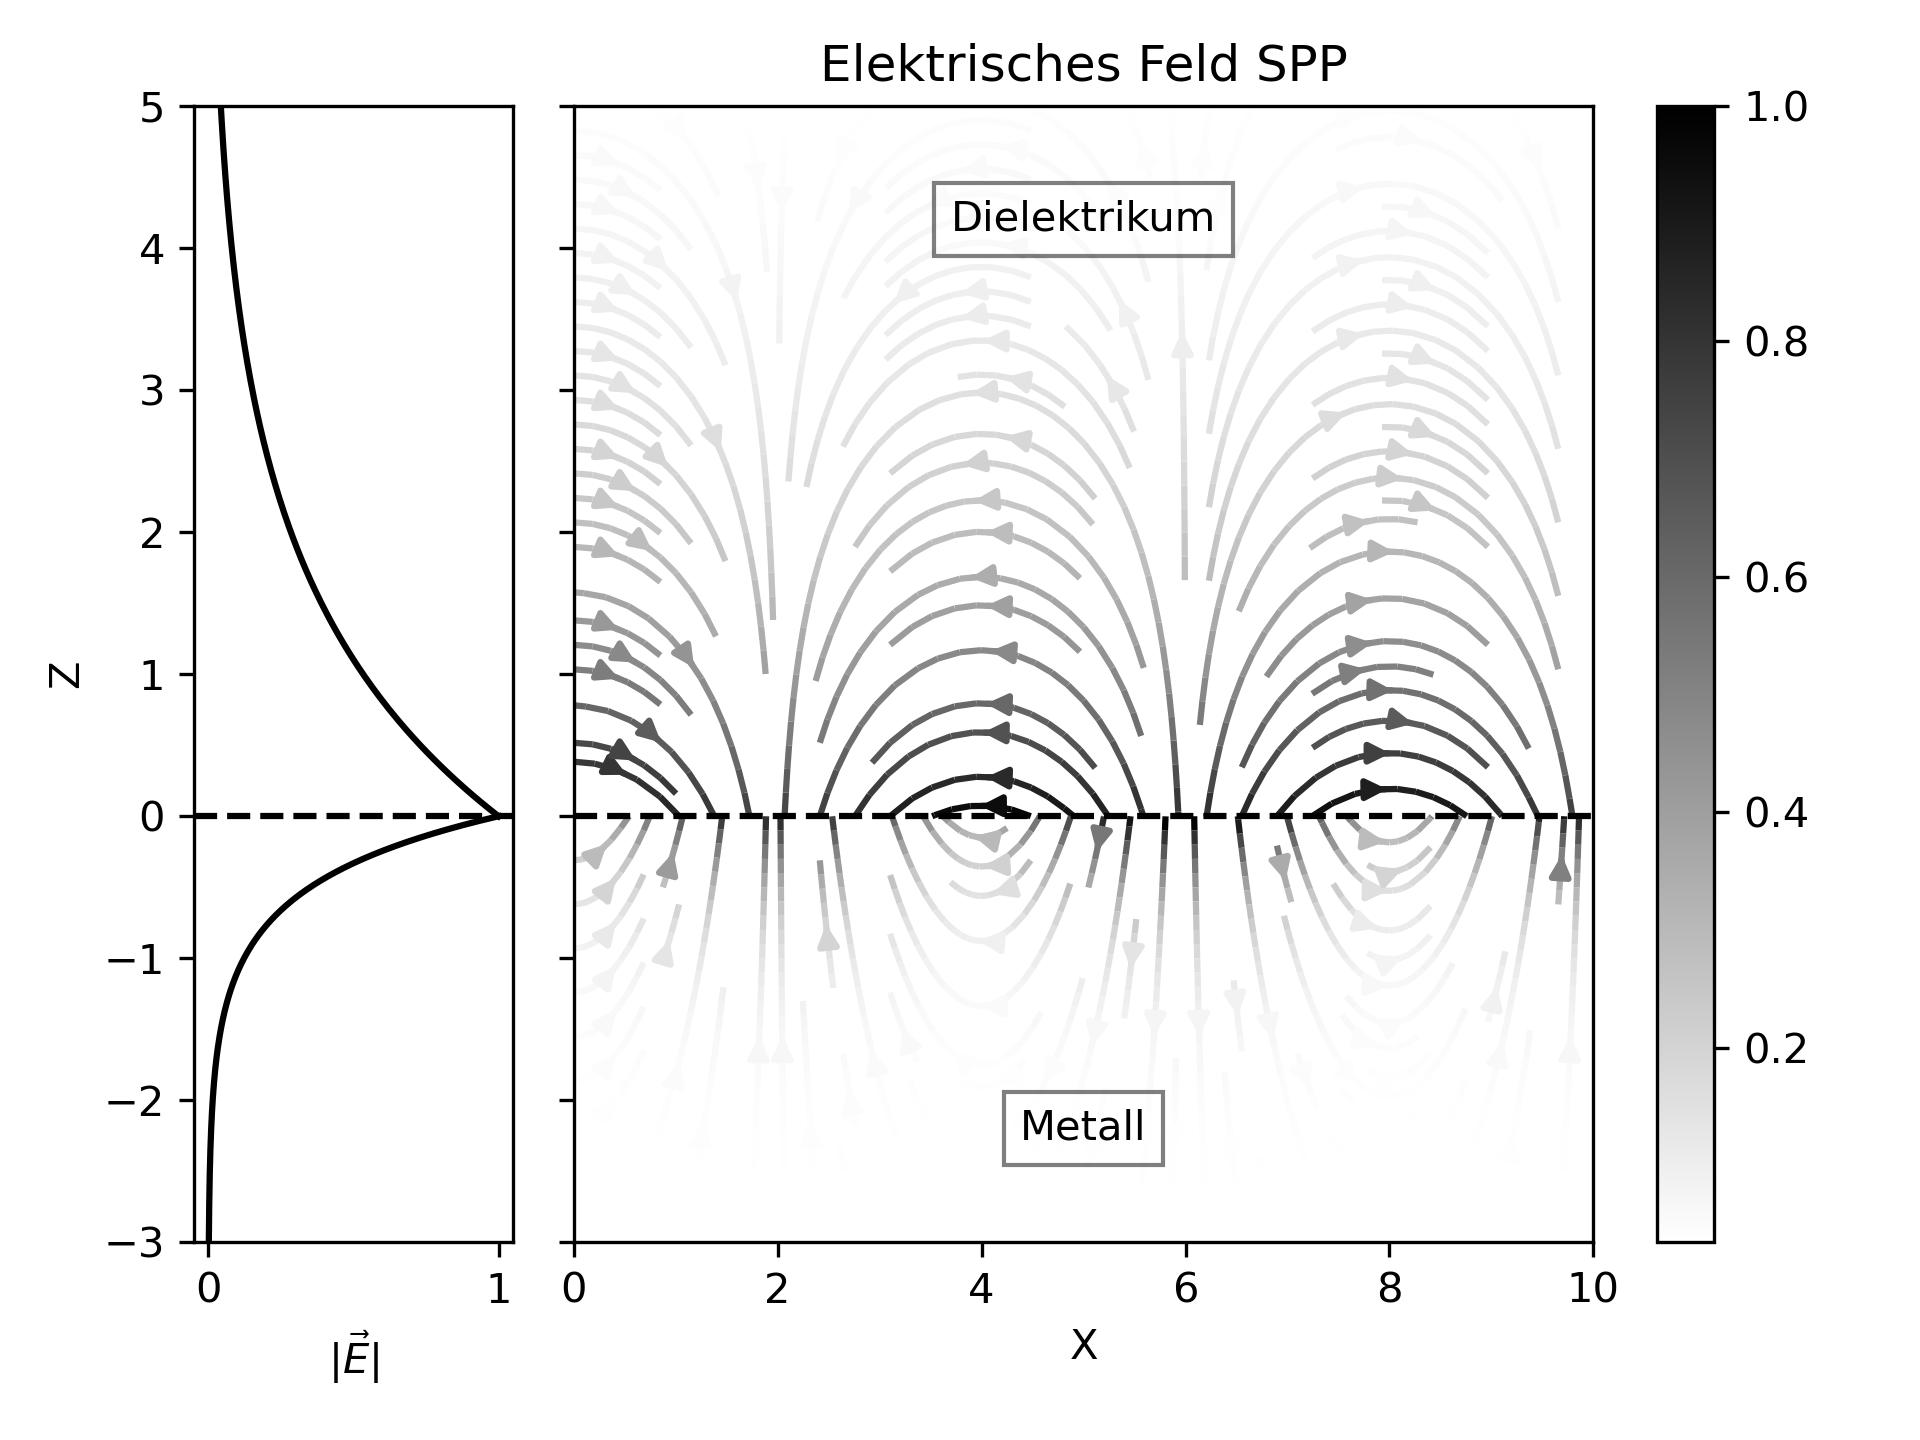
\includegraphics[width=0.7\textwidth]{figures/E_Feld_SPP.png}
		\caption[Elektrisches Feld SPP]{Quantitativer Verlauf der EM-Felder eines SPP entlang einer Metall-Dielektrikums-Grenzschicht. Die Orientierung des elektrischen Felds ist durch die Pfeile dargestellt. Die Grauwert-Skala der Pfeile entspricht dabei dem Betrag der elektrischen Feldstärke. Die Stärke des transversalen Magnetfeldes ist durch die Farbskala dargestellt.}
		\label{fig:electric_field_spp}
	\end{figure}
	
	\subsubsection{SPP Dispersionsrelation}
	Die Herleitung der Dispersionsrelation orientiert sich an den Ausführungen in \cite[pp.~261--ff]{Fox.2020} und kann dort im Detail nachvollzogen werden. Diese Arbeit beschränkt sich daher auf eine kurze Beschreibung des Vorgehens. Damit die oben angesetzten elektromagnetischen Felder \eqref{eq:fields_spp}  die Maxwell-Gleichungen \eqref{eq:maxwell} und die Randbedingungen an der Grenzschicht erfüllen, müssen die Bedingungen \eqref{eq:condition_spp_1},  \eqref{eq:condition_spp_2} gelten. (Hierbei handelt es sich um den Spezialfall nicht-magnetischer Materialien, d.h. $\mu = 1$.)
	\begin{align}
		\label{eq:maxwell}	
		&\vec{\nabla}\cdot\vec{D} = 0		&\vec{\nabla}\cdot\vec{B} = 0 \\
		&\vec{\nabla}\times\vec{E} = -\dfrac{\partial\vec{B}}{\partial t} 
		&\vec{\nabla}\times\vec{H} = 	\dfrac{\partial\vec{D}}{\partial t}\nonumber
	\end{align}
	\begin{subequations}
		\begin{equation}
			\label{eq:condition_spp_1}
			\dfrac{k_{z, \mathrm{M}}}{\epsilon_\mathrm{M}} + \dfrac{k_{z, \mathrm{D}}}{\epsilon_\mathrm{D}} = 0
		\end{equation}		
		\begin{equation}
			\label{eq:condition_spp_2}
			k_{\mathrm{spp}}^2 +k_{z, n}^2 = \epsilon_n\left(\dfrac{\omega}{c}\right)^2; \text{ für  } n=\mathrm{M,D}
		\end{equation}
	\end{subequations}
	Hierbei ist $\vec{D}$ die dielektrische Verschiebung, $\vec{E}$ die elektrische Feldstärke, $\vec{B}$ die magnetische Flussdichte, $\vec{H}$ die magnetische Feldstärke, 	$\epsilon_\mathrm{D}$ die Permittivität des Dielektrikums und $\epsilon_\mathrm{M} = \epsilon_\mathrm{M}(\omega)$ die dielektrische Funktion des Metalls in Abhängigkeit von der Kreisfrequenz der Anregung $\omega$. Durch das Lösen der Bedingungen \eqref{eq:condition_spp_1},  \eqref{eq:condition_spp_2} ergibt sich die Dispersionsrelation des SPP an einer Grenzschicht zwischen einem Metall und einem Dielektrikum zu: 
	\begin{equation}
		\label{eq:dispersion_spp}
		\boxed{
			k_{\mathrm{spp}}\left(\omega\right) = \dfrac{\omega}{c} \sqrt{\dfrac{\epsilon_\mathrm{D}\epsilon_\mathrm{M}(\omega)}{\epsilon_\mathrm{D} + 	\epsilon_\mathrm{M}(\omega)}}  = k_0(\omega) n_{\mathrm{eff}}(\omega)}
	\end{equation}
	Hierbei ist $k_0 = \omega / c$ die Dispersion von elektromagnetischer Strahlung im Vakuum. Und $n_{\mathrm{eff}}(\omega) = \sqrt{\epsilon_\mathrm{D}\epsilon_\mathrm{M}(\omega)/(\epsilon_\mathrm{D} + 	\epsilon_\mathrm{M}(\omega))}$ wird als effektiver Brechungsindex der Anregung bezeichnet. Die Dispersion kann über die Zusammenhänge $E = \hbar \omega$ und $P = \hbar \Re\{k_\mathrm{spp}\}$ auch als Impuls $P(E)$ in Abhängigkeit von der Energie $E$ dargestellt werden.
	
	Aus der Gleichung \eqref{eq:condition_spp_2} folgt $k_{z, n} = \sqrt{\epsilon_n k_0^2 - k_{\mathrm{spp}}^2}$. Diese Beziehung legt den Zusammenhang zwischen $k_{\mathrm{spp}}$ und $k_{z, n}$ fest. Außerdem lässt sich hieraus erkennen, dass für typische Materialien gilt: $ \Im\{k_{z, n}\} \gg \Re\{k_{z, n}\}$. Durch die Dominanz des Imaginärteils über den Realteil der Wellenvektorkomponente senkrecht zur Ausbreitungsrichtung fallen die Amplituden der Felder senkrecht zur Ausbreitungsrichtung exponentiell ab. Diesen Umstand bezeichnet man als Evaneszenz. Die Anregung ist daher eng an der Grenzfläche lokalisiert. 
		
	Im folgenden werden die Messdaten der dielektrischen Funktion von Gold aus der Publikation \cite{Olmon.2012} verwendet, um den Verlauf der Dispersion einer Vakuum-Gold-Mode aus Gleichung \eqref{eq:dispersion_spp} zu berechnen.  Die Publikation stellt Messdaten für unterschiedliche Gold-Oberflächenrauigkeiten zur Verfügung. Es wurden die Messdaten für aufgedampftes Gold verwendet, da die in dieser Arbeit verwendeten Proben bedampft worden sind. Für die Berechnung der Dispersion der Gold-Glas-Mode wurde $\epsilon_\mathrm{D} = 2.327$  verwendet, da dies den verwendeten Proben entspricht. In der Dispersionskurve Abb. \ref{fig:dispersion_spp} ist zu erkennen, dass der Wellenvektor des SPP bei einer Anregungs-Energie von $E = hc/\lambda_{\mathrm{HeNe}}= 1.95\,\mathrm{eV}$ rechts von der Dispersion elektromagnetischer Strahlung im Vakuum liegt. Es tritt bei gegebener Energie also eine Wellenvektor-Differenz zwischen SPP und elektromagnetischer Strahlung auf. Diese $k$-Differenz sorgt dafür, dass SPPs nicht ohne weiteres von elektromagnetischer Strahlung angeregt werden können.
	\begin{figure}[h]		
		\centering
		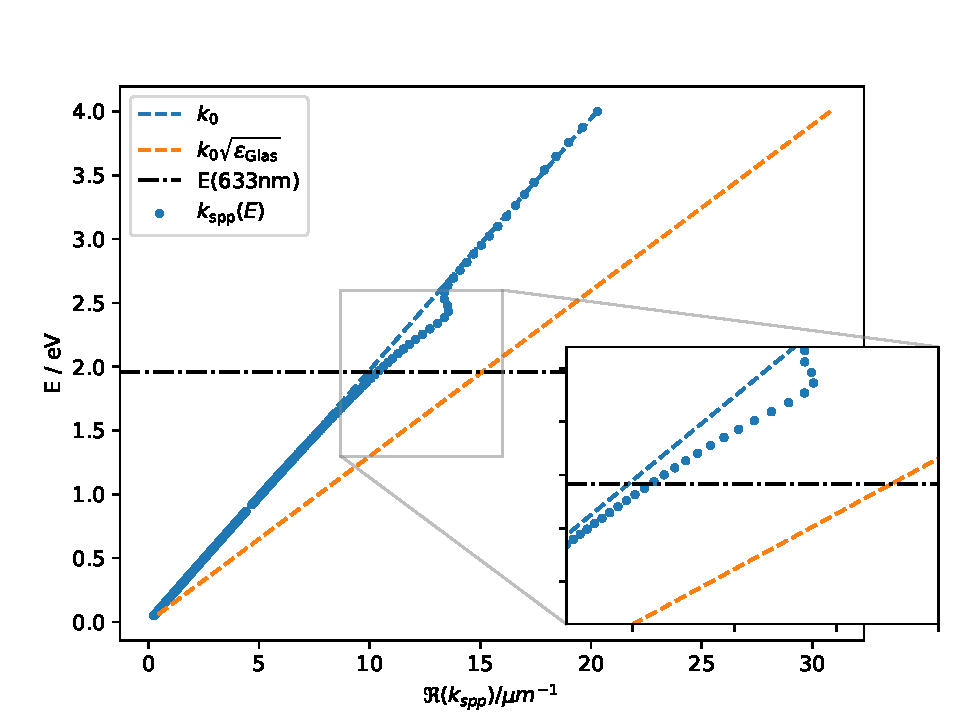
\includegraphics[width=0.7\textwidth]{figures/dispersion.pdf}
		\caption[Dispersion SPP]{Die Abbildung zeigt die mit \eqref{eq:dispersion_spp} und der dielektrischen Funktion von Gold aus \cite{Olmon.2012} berechnete Dispersion für ein SPP an der Grenzschicht zwischen Gold und Vakuum. Außerdem wurde die Dispersion von EM-Strahlung im Vakuum $k_0(E)$ und in Glas $k_0(E)\sqrt{\epsilon_\mathrm{Glas}}$ für $\epsilon_\mathrm{Glas} =2.327$ \cite{Zeiss.} dargestellt, da dieses Glas im weiteren Verlauf der Arbeit als Deckglas der Proben verwendet worden ist. Die Bedeutung der Glas Dispersion wird für das Experiment im Kapitel \ref{sec:leakage_radiation} Leckstrahlung näher erläutert.}
		\label{fig:dispersion_spp}		
	\end{figure}	
	\subsubsection{Anregung von SPPs mittels EM-Strahlung}
	\label{sec:exictation}
	Um trotz der Wellenvektordifferenz in den Dispersionsrelationen SPPs mit elektromagnetischer Strahlung anregen zu können, ist es notwendig, den Wellenvektor der EM-Strahlung anzupassen. Hierfür gibt es unterschiedliche Techniken:
	\paragraph{Kretschmann-Konfiguration}
	In der Kretschmann-Konfiguration wird ausgenutzt, dass für die Anregung von SPPs mit EM-Strahlung nur die Wellenvektorkomponente parallel zur Grenzschichtebene relevant ist. Wie in Abbildung \ref{fig:dispersion_spp} dargestellt, hat EM-Strahlung im Vakuum bei gleicher Energie einen kleineren Wellenvektor als ein SPP an der Grenzschicht Gold-Vakuum. 
	
	In der Kretschmann-Konfiguration wird ein System aus drei Schichten verwendet (Abbildung \ref{fig:kretschman}). Ein dünner Metallfilm wird zwischen zwei Dielektrika ($\mathrm{D}_1$, $\mathrm{D}_2$) mit $\epsilon_{\mathrm{D}_1} > \epsilon_{\mathrm{D}_2}$ eingeschlossen. Das SPP soll hierbei an der Grenzschicht Metall-$\mathrm{D}_2$ propagieren. In der der ersten Schicht wird der Wellenvektor der anregenden EM-Strahlung zunächst auf $k_\mathrm{\mathrm{D}_1} = k_0 \sqrt{\epsilon_\mathrm{D}}$ vergrößert. Die Permittivität $\epsilon_{\mathrm{D}_1}$ wird dabei so gewählt, dass $k_\mathrm{\mathrm{D}_1} = k_0 \sqrt{\epsilon_{\mathrm{D}_1}} > k_\mathrm{SPP}$ gilt. Der Einfallswinkel $\theta_E$ der EM-Strahlung auf die Grenzschichtebene wird dann so festgelegt, dass der auf die Grenzschichtebene projizierte Anteil des Wellenvektors $k_{\mathrm{\mathrm{D}_1}\parallel} = k_{\mathrm{\mathrm{D}_1}} \sin(\theta_E)$ exakt gleich dem Wellenvektor des SPP $k_\mathrm{SPP}$ an der Grenzschichtebene Metall-$\mathrm{D}_2$ ist. Aus dieser Gleichheit ergibt sich die folgende Phasenanpassungsbedingung: 
	\begin{align}
		\label{eq:phase_condition_kretschmann}
		\sin(\theta_E) &= \dfrac{\Re\{k_{\mathrm{spp}}\}}{k_{\mathrm{D}_1}}\\
		\Rightarrow \Re\{k_{\mathrm{SPP}}\} &= \sin(\theta_E) k_0 \sqrt{\epsilon_{\mathrm{D}_1}}
	\end{align}  
	\begin{figure}[h] 
		\centering
		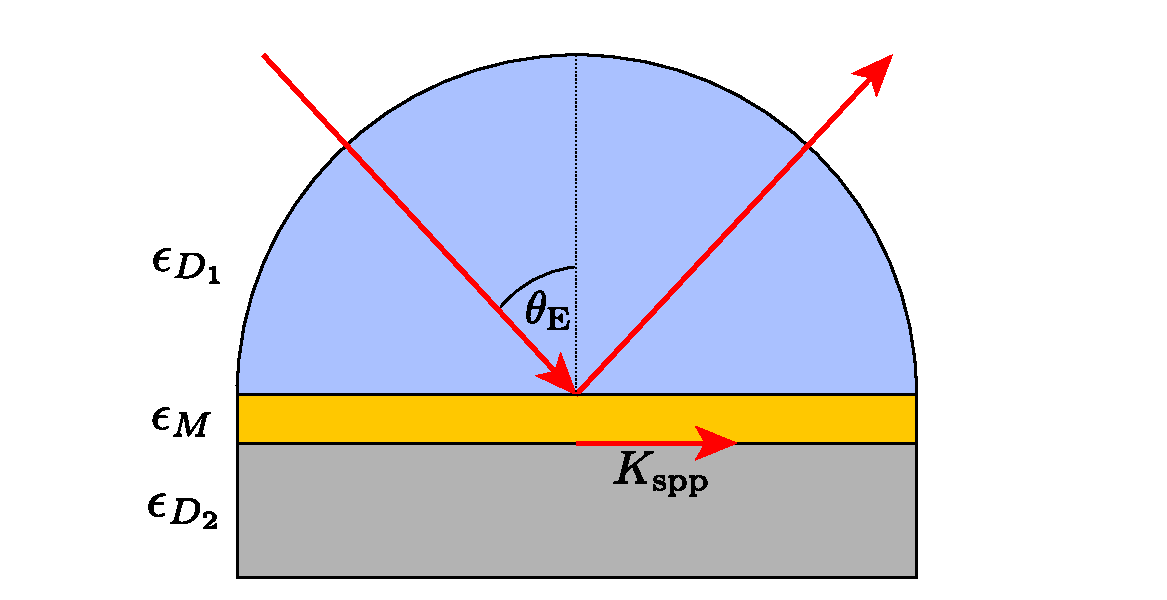
\includegraphics[width=0.5\textwidth]{figures/Kretschmann.pdf}
		\caption[Kretschmann-Konfiguration]{Schematischer Aufbau der Kretschmann-Konfiguration. Die Anregungsstrahlung tritt hier zunächst in das Medium mit $\epsilon_{\mathrm{D}_1}$ ein. Hierdurch wird der Wellenvektor der Anregungsstrahlung auf $k_{\mathrm{D}_1}=k_0\sqrt{\epsilon_{\mathrm{D}_1}}$ vergrößert. $\mathrm{D}_1$ wird so gewählt, dass $k_{\mathrm{D}_1}> k_{\mathrm{SPP}}$ gilt. ($k_{\mathrm{SPP}}$ bezieht sich hierbei auf die Mode Metall-Dielektrikum 2 und ergibt sich aus \eqref{eq:dispersion_spp}). Der Einfallswinkel $\theta_E$ wird so gewählt, dass die Projektion von $k_{\mathrm{D}_1}$ auf die Goldoberfläche exakt $k_{\mathrm{SPP}}$ entspricht. Die Abbildung ist an \cite{Jaruschewski.2020} angelehnt.}
		\label{fig:kretschman}
	\end{figure}
	Der Anregungsmechanismus in der Kretschmann-Konfiguration kann mit Hilfe des in Abbildung \ref{fig:dispersion_spp} dargestellten Dispersionsverhalten von SPPs und EM-Strahlung für ein Vakuum-Gold-Glas System mit einem Helium-Neon Laser (He-Ne Laser) der Wellenlänge $\lambda_{\mathrm{HeNe}}=633\,\mathrm{nm}$ auch grafisch verdeutlicht werden: Der Wechsel der EM-Strahlung aus dem Vakuum in das Glas führt dazu, dass $k$ von dem Schnittpunkt der blauen Kurve $k_0$ mit $E(633 \, \mathrm{nm})$ auf den Schnittpunkt der orangenen Kurve $k_0(E)\sqrt{\epsilon_\mathrm{Glas}}$ mit $E(633 \, \mathrm{nm})$ wechselt. Die Projektion von $k_{\mathrm{Glas}\parallel}$ auf die Grenzfläche bei Variation des Einfallswinkels $\theta_E$ entspricht dann einer Rotation von $k_0(E)\sqrt{\epsilon_\mathrm{Glas}}$ gegen den Uhrzeigersinn um den Ursprung. Der Einfallswinkel  $\theta_E$ und damit auch die Rotation der Glas-Dispersion wird nun über Phasenanpassungsbedingung \eqref{eq:phase_condition_kretschmann} so gewählt, dass $k_{\mathrm{Glas}\parallel}$ bei der Energie $E=E(633\,\mathrm{nm})$ einen Berührpunkt mit der Dispersion $k_\mathrm{spp}$ des SPP hat.
	Bei der Reflexion einer elektromagnetischen Welle an einem Metall dringen in das Metall evaneszente Felder ein \cite{Novotny.2012b}. Ist die Metallschicht ausreichend dünn, haben diese evaneszenten Felder an der Grenzfläche Metall-$\mathrm{D}_2$ noch genügend Feldstärke, um dort ein SPP anzuregen. Dies ist nur möglich, da die Wellenvektorkomponente parallel zur Grenzschichtebene wie oben erläutert, an das SPP angepasst worden ist. Die in Abb. \ref{fig:kretschman} gezeigte Geometrie nutzt für $\mathrm{D}_1$ einen Halbkreis, damit der Strahl unabhängig vom Winkel $\theta_\mathrm{E}$ senkrecht in $\mathrm{D}_1$ eintritt.
	\paragraph{Anregung an Strukturen}
	Eine weitere Möglichkeit, die Wellenvektordifferenz zu überwinden, stellen scharfe Strukturen in oder an der Metalloberfläche dar. Räumliche Diskontinuitäten von $\epsilon(\vec{r},\omega)$ führen dazu, dass die Impulserhaltung, welche erst zu einer Erhaltung des Wellenvektors geführt hat, lokal außer Kraft gesetzt werden kann. Um nun abschätzen zu können, ob eine räumliche Diskontinuität von $\epsilon(\vec{r},\omega)$ eine hinreichend große Impulsdifferenz zwischen SPP und EM-Strahlung überwinden kann, muss eine räumliche Fouriertransformation von $\epsilon(\vec{r},\omega)$ gebildet werden. Scharfe Strukturen im Ortsraum besitzen gemäß den Gesetzen der Fouriertransformation ein breites Raumfrequenzspektrum. Dieses breite Raumfrequenzspektrum sorgt dafür, dass die nötige Wellenvektordifferenz überwunden werden kann, um ein SPP anzuregen. Der Streuprozess von einem Photon an einem kleinem Partikel auf der Goldoberfläche kann in erster Näherung auch als abstrahlender Dipol aufgefasst werden, dessen EM-Strahlung wiederum ein breites Raumfrequenzspektrum aufweist. Dieser Prozess wird detaillierter in Abschnitt \ref{sec:spatial_freq_dip} anhand des Raumfrequenzspektrums eines Dipols dargestellt.
	\subsubsection{Leckstrahlung}
	\label{sec:leakage_radiation}
	Leckstrahlung ist der inverse Effekt zur Anregung in der Kretschmann-Konfiguration. In einem Dreischichtsystem $\mathrm{D}_2$-Metall-$\mathrm{D}_1$, bestehend aus einem Metall und zwei Dielektrika ($\mathrm{D}_1$, $\mathrm{D}_2$), kann ein an der Grenzfläche $\mathrm{D}_2$-Metall propagierendes SPP evaneszente EM-Felder erzeugen, die bis zur Grenzfläche Metall-$\mathrm{D}_1$ vordringen können (Abbildung \ref{fig:leakage_radiation}). Damit diese Felder trotz der Evaneszenz die Grenzfläche Metall-$\mathrm{D}_1$ erreichen, ist es notwendig, dass die Metallschicht hinreichend dünn ist. Diese Felder können EM-Strahlung in $\mathrm{D}_1$ unter dem Winkel $\theta_\mathrm{L}$ hervorrufen. Damit der Wellenvektor des SPP und die zur Grenzschicht parallelen Komponenten des Wellenvektors der Leckstrahlung übereinstimmen, muss dieser Winkel analog zu \eqref{eq:phase_condition_kretschmann} folgende Phasenanpassungsbedingung erfüllen:
	\begin{equation}
		\label{eq:phase_condition}
		\boxed{\Re\{k_{\mathrm{spp}}\}=\sin(\theta_\mathrm{L}) k_0 \sqrt{\epsilon_{\mathrm{D}_1}}}
	\end{equation}
	
	Dies ist nur möglich, wenn gilt: {$\sqrt{\epsilon_{\mathrm{D}_1}} > \Re\{n_\mathrm{eff, spp}\}$}. Diese in das Dielektrikum $\mathrm{D}_1$ abgegebene Strahlung bezeichnet man als Leckstrahlung. Durch die Phasenanpassungsbedingung \eqref{eq:phase_condition} kann einem bestimmten Abstrahlwinkel $\theta_L$ ein konkreter $\Re\{k_{\mathrm{spp}}\}$ zugeordnet werden und umgekehrt. Dieser Umstand wird bei der Leckstrahlmikroskopie genutzt, um den Wellenvektor des SPP zu bestimmen.
	Die Phasenanpassungsbedingung \eqref{eq:phase_condition} kann, wie in \cite{Burke.1986} gezeigt wird, durch eine Fouriertransformation verallgemeinert werden. So erhält man den Ausdruck \eqref{eq:ext_phase_condition} für die winkelabhängige Abstrahlung von Leckstrahlung einer SPP-Mode mit bekanntem Wellenvektor $k_{\mathrm{SPP}} \in \mathbb{C}$
	\begin{equation}
		\label{eq:ext_phase_condition}
		I(\theta) = \dfrac{\text{const.}}{\left(k_{\parallel}(\theta) - \Re\{k_{\mathrm{SPP}}\}\right)^2 + (\Im\{k_{\mathrm{SPP}}\})^2}
	\end{equation}
	Hierbei ist $k_{\parallel}(\Theta) = k_{\mathrm{D}_1}\sin(\Theta)$ der Wellenvektor-Anteil der Leckstrahlung parallel zur Grenzfläche. Die Winkelabhängigkeit der Leckstrahlung wird also durch ein Lorentz-Profil mit Maximum bei $\Theta = \theta_\mathrm{L}$ beschrieben. Die Profilbreite wird durch den Imaginärteil von $k_{\mathrm{SPP}}$ (also der Dämpfung der Mode) bestimmt. Die Beobachtung von Leckstrahlung mit optischen Instrumenten ist durch diese Zusammenhänge ein nützliches Werkzeug, um Rückschlüsse auf die Eigenschaften des SPP zu ziehen.
	\begin{figure}[h] 
		\centering
		\includegraphics[width=0.5\textwidth]{figures/leckstrahlung.pdf}
		\caption[Leckstrahlung Drei-Schichtsystem]{Die Abbildung zeigt die Abstrahlung von Leckstrahlung in einem Drei-Schichtsystem. An einem Defekt auf der Metalloberfläche wird mit einem Laser ein SPP angeregt (siehe Abschnitt \ref{sec:exictation}). Das SPP propagiert an der Grenzschicht $\mathrm{D}_2$-Metall und strahlt unter dem Winkel $\theta_L$ Leckstrahlung in das Dielektrikum $\mathrm{D}_1$ ab. Der Winkel $\theta_L$ ergibt sich dabei aus der Phasenanpassungsbedingung \eqref{eq:phase_condition}}.
		\label{fig:leakage_radiation}
	\end{figure}
	\subsubsection{Berechnung von charakteristischen Größen für das System Luft-Gold-Glas}
	Alle in dieser Arbeit durchgeführten Messungen wurden am System Luft-Gold-Glas durchgeführt. Daher werden an dieser Stelle die oben eingeführten Größen für dieses System angegeben. Die Dielektrizitätskonstante des Glases ist $\epsilon_{\mathrm{G}} = 2.327$ \cite{Zeiss.}, die von Luft beträgt $\epsilon_{\mathrm{L}} = 1.00059$ \cite{Hippel.1995}. Die dielektrische Funktion von Gold wurde bei einer Anregungsenergie von $E_{\mathrm{HeNe}} = h\lambda/c = 1.96\,\mathrm{eV} $ durch Interpolation der Messdaten aus der Publikation \cite{Olmon.2012} berechnet: $\epsilon_{\mathrm{Au}}(1.96\mathrm{eV}) = -12.04 +1.163i$. Aus diesen Daten lassen sich nun folgende Größen berechnen:
	\begin{subequations}
		\begin{align}
			n_{\mathrm{eff}} &= \sqrt{\dfrac{\epsilon_{\mathrm{L}}\epsilon_{\mathrm{Au}(\omega)}}{\epsilon_{\mathrm{L}} + 	\epsilon_{\mathrm{Au}}(\omega)}} = 	1.044 + 0.005i \label{eq:theo_n_eff}\\			
			\theta_\mathrm{L} &=  \arcsin\left(\dfrac{\Re(n_{\mathrm{eff}})}{ n_\mathrm{G}}\right) = 43.2^\circ 
			\label{eq:theo_theta_l}\\
			k_{\mathrm{SPP}} &= k_0 n_{\mathrm{eff}} = (10.365 + 0.0449i)\,\mathrm{\mu m}^{-1}\label{eq:theo_k_spp}
		\end{align}
	\end{subequations}
	\subsection{Plasmonischer Spin-Hall-Effekt (PSHE)}
	Als PSHE wird bezeichnet, dass an einer räumlich symmetrischen Struktur angeregte SPP, abhängig von der Polarisation der anregenden Strahlung, bevorzugt in eine bestimmte Richtung propagieren. Speziell propagiert ein SPP das mit links-zirkular polarisierter Anregungsstrahlung erzeugt worden ist in die entgegengesetzte Richtung zu dem SPP, welches mit rechts-zirkular polarisierter Strahlung angeregt worden ist (Abbildung \ref{fig:spin_hall_schema}). Der PSHE kann durch zwei verschiedene Vorgehensweisen erklärt werden. Ein Weg ist es, die Strahlung, die von der Struktur ausgeht, an welcher SPP angeregt werden, durch einen zirkular polarisierten Dipol zu nähern. Das Fernfeld eines zirkular polarisierten Dipols ist isotrop. Daher ist es zunächst verwunderlich, dass ein zirkular polarisierter Dipol zu einer gerichteten Anregung führen kann. Bei genauerem Betrachten des Dipol-Feldes fällt allerdings auf, dass das Nahfeld nicht isotrop ist. Wenn nun ein SPP unterstützendes Schichtsystem in dieses Nahfeld des Dipols gebracht wird, kann diese Nahfeld-Anisotropie zu einer gerichteten Anregung führen.
	Eine weitere Vorgehensweise, den Effekt zu erklären, geht von der Erhaltung des Drehimpulses aus. Das Photon hat vor der Wechselwirkung mit der Struktur einen longitudinalen Drehimpuls, der je nach Helizität der zirkularen Polarisation in oder entgegen der Ausbreitungsrichtung des Photons zeigt. Das SPP hingegen hat einen Drehimpuls, der transversal auf seiner Ausbreitungsrichtung steht (siehe Abschnitt \ref{sec:spin_spp}). Damit der Drehimpuls nach der Wechselwirkung erhalten bleibt, ist also Änderung der Propagationsrichtung notwendig.
	(vgl. Spin Hall Effekt)
	\subsubsection{Raumfrequenzspektrum von elektromagnetischen Feldern}
	Um den PSHE zu verstehen, wird die Raumfrequenzdarstellung von elektromagnetischen Feldern benötigt. Die folgenden Ausführungen orientieren sich an \cite{Novotny.2012b}, wobei in dieser Arbeit nur der etwas einfachere 2D-Fall diskutiert wird.\\		
	Das elektrische Feld am Ort $\vec{r} = (x, z) $ sei durch $\vec{E}({\vec{r}})$ gegeben.
	Die Zeitabhängigkeit von $\vec{E}$ sei durch $\vec{E}({\vec{r}, t})=\Re\{\vec{E}({\vec{r}})\exp(-i\omega t)\}$ beschrieben. Dann lässt sich $\vec{E}({\vec{r}})$ durch eine Fouriertransformation in $x$-Richtung wie folgt darstellen:
	\begin{equation}
		\label{eq:Exz_fourier}
		\vec{E}(x,z) = \int_{-\infty}^{\infty}\mathrm{d}{k_x}\hat{\vec{E}}(k_x,z)\exp(ik_xx)				
	\end{equation}
	\begin{equation}
		\label{eq:EKxz_fourier}
		\hat{\vec{E}}(k_x,z) = \dfrac{1}{2\pi}\int_{-\infty}^{\infty}\mathrm{d}x\vec{E}(x,z)\exp(-ik_xx)
	\end{equation}
	Wenn wir davon ausgehen, dass das Medium entlang der $x$-Achse homogen, isotrop, linear und quellfrei ist, muss das elektrische Feld die sich unter diesen Bedingungen aus den Maxwell-Gleichungen \eqref{eq:maxwell} ergebende Helmholtz-Gleichung $(\vec{\nabla}^2+k^2)\vec{E}({\vec{r}}) = 0$ erfüllen. Einsetzen von \eqref{eq:Exz_fourier} in die Helmholtz-Gleichung ergibt mit der Definition $k_z := \sqrt{k^2-k_x^2}$ folgenden Zusammenhang:
	\begin{equation}
		\label{eq:spatial_spektrum}
		\hat{\vec{E}}(k_x,z) =\hat{\vec{E}}(k_x,z= 0) \exp(\pm ik_ z)
	\end{equation}
	Das Vorzeichen legt hier die Propagationsrichtung fest.
	Einsetzen in \eqref{eq:Exz_fourier} ergibt:
	\begin{equation}
		\label{eq:Espatial_spektrum}
		\vec{E}(x,z) = \int_{-\infty}^{\infty}\mathrm{d}{k_x}\hat{\vec{E}}(k_x,z= 0)\exp(i(k_xx\pm k_ z))
	\end{equation}
	Wenn also das Raumfrequenzspektrum für einen z-Wert bekannt ist, lassen sich die Spektren für alle anderen z-Werte gemäß \eqref{eq:spatial_spektrum} berechnen. Für einen festen Wert von $k_x$ gibt es, je nachdem ob $k_x$ größer oder kleiner als $k$ ist, zwei unterschiedliche Lösungsarten: Wenn $k_x^2 < k^2$ gilt, ist $k_z = \sqrt{k^2-k_x^2}$ eine reelle Zahl. Daher handelt es sich nach \eqref{eq:spatial_spektrum} um eine ebene Welle, die entlang der z-Achse propagiert.
	Wenn hingegen $k_x^2 > k^2$ gilt, ist $k_z = \sqrt{k^2-k_x^2}$ eine imaginäre Zahl. Dann handelt es sich bei \eqref{eq:spatial_spektrum} um eine evaneszente Welle, die entlang der z-Achse exponentiell abklingt. In dem Raumfrequenzspektrum kann man also zwischen Bereichen mit ebenen Wellen und Bereichen mit evaneszenten Wellen unterscheiden. Dieses Konzept lässt sich ohne weiteres auch auf drei Raumdimensionen und das magnetische Feld erweitern.
	\subsubsection{Raumfrequenzspektrum der elektromagnetischen Strahlung eines oszillierenden Dipols}
	\label{sec:spatial_freq_dip}
	Durch das oben beschriebene Verfahren lässt sich das Raumfrequenzspektrum eines beliebig polarisierten Dipols bestimmen. Unter einem polarisierten Dipol versteht man die Überlagerung zweier Dipole, die mit gleicher Frequenz, aber mit beliebiger Phasendifferenz und Amplitude schwingen. Dieses Dipolmoment lässt sich durch folgenden Ausdruck darstellen (diese Arbeit beschränkt sich dabei wieder auf den 2D-Fall): 
	$$\vec{P}(t)= \Re\biggl\{\underbrace{\begin{pmatrix} p_x \\ p_z \end{pmatrix}}_{\vec{P}} \exp(-i\omega t)\biggr\} $$
	$p_x$ und $p_y$ sind im allgemeinen komplexe Zahlen. So kann $\vec{P}$ auch elliptische Polarisationen darstellen. Die y-Komponente des Magnetfeldes dieses Dipols lässt sich nun, wie in \cite{Novotny.2012b} und \cite{RodriguezFortuno.2013} gezeigt wird, analog zu den obigen Ausführungen in Raumfrequenzanteile zerlegen.
	\begin{equation}
		H_y(x, z) = \int_{-\infty}^{\infty}\mathrm{d}k_x\hat{H_y}(k_x, z)\exp(ik _xx) 
	\end{equation}
	mit
	\begin{equation}
		\label{eq:spatial_freq_dip}
		\boxed{\hat{H_y}(k_x, z) = \dfrac{i\omega}{8\pi^2}\left(p_z\dfrac{k_x}{k_z} \mp p_x\right)\exp(ik_z|z-z_{\mathrm{Dipol}}|)}
	\end{equation}
	$z_{\mathrm{Dipol}}$ ist hierbei die Position des Dipols auf der $z$-Achse. $k_z$ lässt sich wieder über die Differenz von $k_x$ zur Gesamtwellenzahl $k$ berechnen $k_z := \sqrt{k^2-k_x^2}$. Wenn $k_x$ schon den gesamten Anteil der Gesamtwellenzahl 'aufbraucht',  wird $k_z$ imaginär. Hierdurch klingt der Beitrag von $\hat{H_y}(k_x, z)$ mit zunehmendem $z$ ab. Deswegen bezeichnet man die resultierende Welle als evaneszent. Diese Wellen können nicht über weite Strecken propagieren und beeinflussen deswegen nur das Nahfeld. Wenn $k_x$ einen Anteil von der Gesamtwellenzahl 'übrig' lässt, bleibt $k_z$ reell und die Welle kann propagieren. Ähnlich wie bei der Leckstrahlung ergibt sich durch die Phasenanpassungsbedingung ein Winkel zur $z$-Achse, unter dem die Welle mit bestimmten $k_x$ propagiert: $\Theta = \arcsin(k_x/k)$. Da $k = \omega / c$ gilt, hängt das Raumfrequenzspektrum nur von dem äußeren Parameter $\omega$ bzw. $k$ ab. 
	\paragraph{Numerische Analyse des Dipol-Raumfrequenzspektrums}
	Die Analyse des Raumfrequenzspektrums erfolgt in dieser Arbeit rein quantitativ unter Verwendung von willkürlichen Einheiten. Hierfür wurde \eqref{eq:spatial_freq_dip} für festgelegte Größen numerisch ausgewertet.
	Das Raumfrequenzspektrum wurde entlang der $z = 0$ 'Ebene' (im 2D Fall eine Gerade) dargestellt. Der Dipol wurde in einer Entfernung von $d = 0.1 \lambda$  von dieser Ebene auf der $z$-Achse positioniert. $k_x$ wurde hierbei in Einheiten von $k$ dargestellt. Dann ist für das Intervall $-1 < k_x / k <1$ der Wert von $k_z$ reell. Dieses $k_x$-Intervall entspricht also propagierenden Wellen. Die Raumfrequenzspektrums-Amplitude wurde im Bereich der Darstellung auf $1$ normiert. Außerdem wurden Real- und Imaginärteil der Raumfrequenzamplitude getrennt voneinander dargestellt.
	\subparagraph{Linear polarisierter Dipol in $x$-Richtung}
	Der Dipol sei:
	$$\vec{P} = \begin{pmatrix} 1 \\ 0\end{pmatrix}$$
	Das Raumfrequenzspektrum des in x-Richtung orientierten Dipols ist in \ref{fig:spatial_spectrum_x} dargestellt und weist eine gerade Parität auf, ist also achsensymmetrisch.	
	\subparagraph{Linear polarisierter Dipol in $z$-Richtung}
	Der Dipol sei:
	$$\vec{P} = \begin{pmatrix} 0 \\ -i\end{pmatrix}$$
	Das Raumfrequenzspektrum dieses Dipols ist in \ref{fig:spatial_spectrum_z} dargestellt und zeigt ungerade Parität, ist also punktsymmetrisch bezüglich des Ursprungs.
	\begin{figure}
		\centering
		\label{fig:spatial_spectrum_zx}
		\begin{subfigure}[h]{0.49\textwidth}
			\centering
			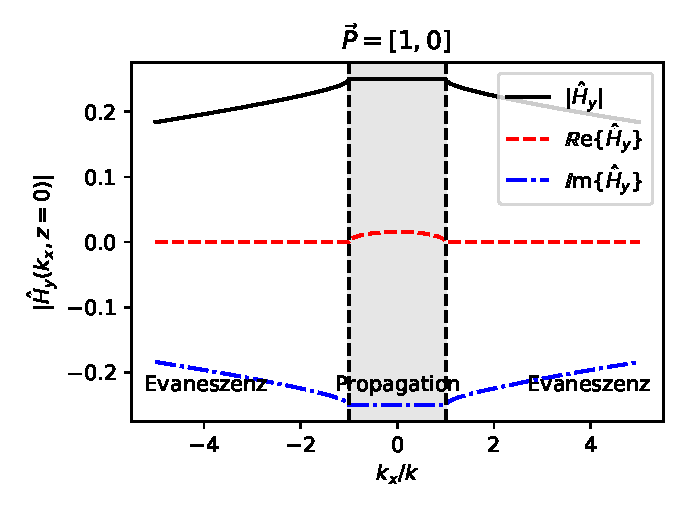
\includegraphics[width=\textwidth]{figures/spatial_spectrum_x.pdf}
			\caption{Orientierung in x-Richtung}
			\label{fig:spatial_spectrum_x}
		\end{subfigure}		
		\begin{subfigure}[h]{0.5\textwidth}
			\centering
			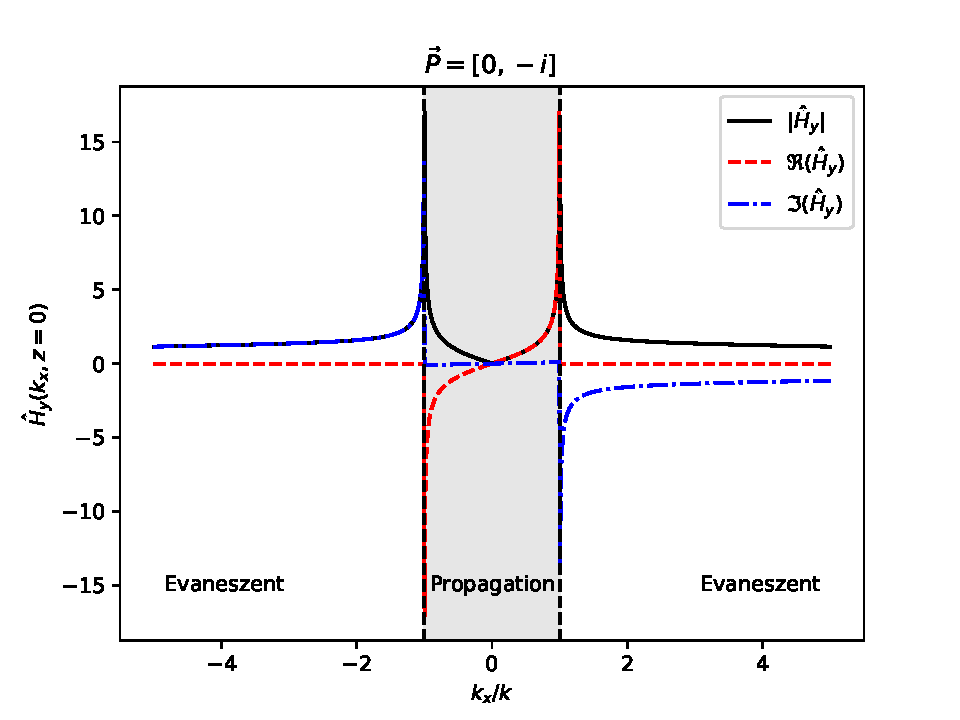
\includegraphics[width=\textwidth]{figures/spatial_spectrum_z.pdf}
			\caption{Orientierung in z-Richtung}
			\label{fig:spatial_spectrum_z}
		\end{subfigure}		
		\caption[Raumfrequenzspektrum linear polarisierter Dipol]{Das Raumfrequenzspektrum eines linear polarisierten Dipols zeigt je nach  dessen Orientierung unterschiedliche Parität. In rot ist jeweils der Realteil, in blau der Imaginärteil und in schwarz der Betrag der jeweiligen Raumfrequenzamplitude dargestellt.}		
	\end{figure}
	\subparagraph{Zirkular polarisierter Dipol}
	Der Dipol sei:
	$$\vec{P} = \begin{pmatrix} 1 \\ -i\end{pmatrix}$$
	Das Raumfrequenzspektrum (Abb. \ref{fig:spatial_spectrum_circ}) aus dieser phasenverschobenen Überlagerung der beiden Dipole ist asymmetrisch.  Im negativen x-Bereich überlagern sich die Spektren destruktiv, im positiven Bereich konstruktiv. Wenn nun sehr nah an diesem zirkular polarisierten Dipol ein Schichtsystem positioniert wird, welches die Anregung von SPP unterstützt, kann durch den Teil des Spektrums, der $k_{\mathrm{SPP}}$ entspricht, ein SPP angeregt werden. Das Vorzeichen von $k_{\mathrm{SPP}}$ entspricht hierbei der Propagationsrichtung des SPP. Weil $\hat{H}_y(k_{\mathrm{SPP}}) \neq \hat{H}_y( -k_{\mathrm{SPP}}) $ gilt, findet die Anregung bevorzugt in eine bestimmte Propagationsrichtung statt. Diese Richtung ist abhängig von dem Drehsinn des zirkular polarisierten Dipols.			
	Das Nahfeld eines zirkular polarisierten Dipols ist also anisotrop, obwohl das Fernfeld, welches man durch Substitution von $k_x = k_o \sin(\theta)$ erhält, isotrop ist.
	
	Damit die hier angenommene Orientierung des Dipols in der Struktur zur $z$-Ebene und damit auch zur Metalloberfläche auftritt, ist ein nicht senkrechter Einfall der anregenden Strahlung notwendig. Es ist zu erwarten, dass der PSHE ausgeprägter wird, je flacher der Einfallswinkel zur Oberfläche gewählt wird. Erst dieser nicht senkrechte Einfall erzeugt den Bruch der Symmetrie, welcher eine Unterscheidung der beiden Anregungsrichtungen ermöglicht.
	\begin{figure}[h]
		\centering
		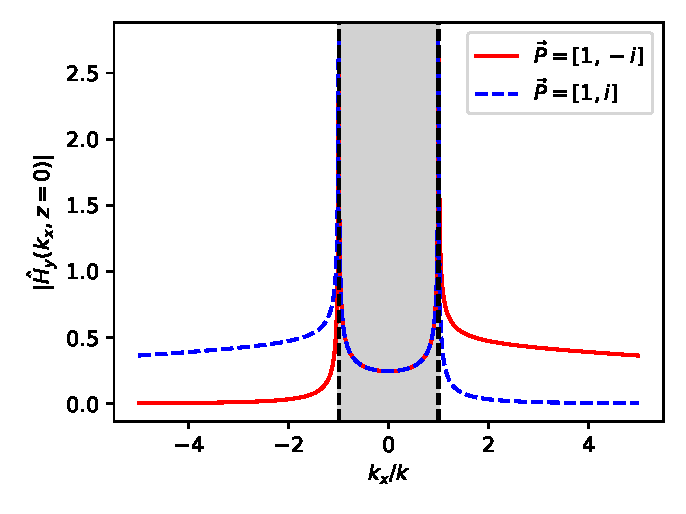
\includegraphics[width=0.7\textwidth]{figures/spatial_spectrum_circ.pdf}
		\caption[Raumfrequenzspektrum zirkular polarisierter Dipol]{Raumfrequenzspektrum eines zirkular polarisierten Dipols für links- und rechts-zirkulare Polarisation}
		\label{fig:spatial_spectrum_circ}
	\end{figure}	
	
	
	
	\subsubsection{Analyse des Drehimpulses von elektromagnetischer Strahlung}
	\label{sec:spin_spp}
	Elektromagnetische Strahlung kann Impuls und Drehimpuls transportieren. Der Drehimpuls übersetzt sich nach dem quantenmechanischen Korrespondenzprinzip in einen Spin. Im folgenden wird daher im klassischen Bild der Drehimpuls von unterschiedlichen elektromagnetischen Strahlungsarten analysiert.
	\paragraph{Propagierende Ebene-Wellen}
	Propagierende EM-Wellen transportieren abhängig von ihrer Polarisation ein Drehimpuls. Linear polarisierte EM-Wellen besitzen kein Drehimpuls. Ihr elektrischer und magnetischer Feldvektor oszilliert jeweils nur in einer Ebene.
	
	Bei elliptisch polarisierten elektromagnetischen Wellen hingegen rotiert der elektrische Feld-Vektor in einer Ebene senkrecht zur Ausbreitungsrichtung. Das gleiche gilt auch für den magnetischen Feldvektor. Diese Felder können daher ein Referenzteilchen in Rotation versetzten und transportieren dementsprechend auch einen Drehimpuls. Da die Rotation nur in Ebenen senkrecht zur Ausbreitungsrichtung stattfindet, ist der Drehimpuls parallel bzw. antiparallel zur Ausbreitungsrichtung der EM-Welle orientiert. Daher haben elliptisch polarisierte propagierende elektromagnetische Felder einen longitudinalen Drehimpuls. (Abbildung \ref{fig:prop_spin})
	
	\begin{figure}[h]
		\centering
		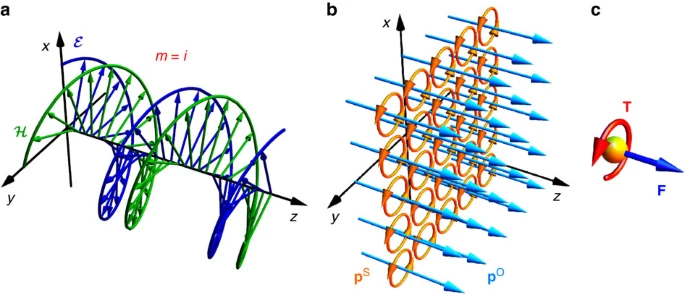
\includegraphics[width=0.7\linewidth]{figures/spin/prop_spin}
		\caption[Spin propagierende EM-Welle]{Der elektrische Feldvektor einer propagierenden, zirkular polarisierten Welle beschreibt bei festgehaltener Zeit eine Helix-Bahn entlang der Ausbreitungsrichtung. An einem festgehaltenen Ort beschreibt der elektrische Feldvektor also bei fortlaufender Zeit eine Kreisbahn senkrecht zur Ausbreitungsrichtung. Die Abbildung ist aus \cite{Bliokh.2014} übernommen.}
		\label{fig:prop_spin}
	\end{figure}
	
	\paragraph{Evaneszente Felder}	
	Evaneszente elektromagnetische Felder weisen hingegen unabhängig von ihrer Polarisation einen Spin in transversaler Richtung auf. Wenn man bei einer evaneszenten elektromagnetischen Welle den zeitlichen Verlauf des elektrischen Feldvektors $\vec{E}(t)$ an einem festen Ort beobachtet, stellt man fest, dass $\vec{E}(t)$ in einer Ebene die in Ausbreitungsrichtung liegt, aber senkrecht zum Magnetfeld orientiert ist, rotiert. Der elektrische Feldvektor dreht sich hier also in einer Ebene parallel zur Ausbreitungsrichtung (Abbildung \ref{fig:ev_spin}). Der Drehimpuls steht dementsprechend senkrecht auf der Ausbreitungsrichtung \cite{Bliokh.2014}. Da SPPs aus Evaneszenten Feldern bestehen weisen SPPs einen transversalen Drehimpuls auf. 
	
	\begin{figure}[h]
		\centering
		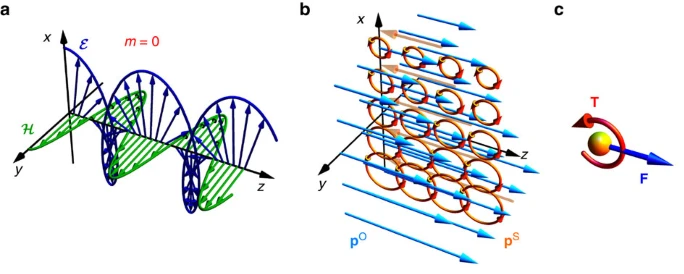
\includegraphics[width=0.7\linewidth]{figures/spin/ev_spin}
		\caption[Spin evaneszente EM-Welle]{Der elektrische Feldvektor einer evaneszenten Welle beschreibt bei festgehaltener Zeit eine Zykloide in der $xz$-Ebene. An einem festgehaltenen Ort beschreibt der elektrische Feldvektor also mit fortschreiten der Zeit eine Kreisbahn in der $xz$-Ebene. Die Abbildung ist aus \cite{Bliokh.2014} übernommen.}
		\label{fig:ev_spin}
	\end{figure}

	\paragraph{Drehimpulserhaltung beim PSHE}
	Durch den streifenden Einfall des zirkular polarisierten Lasers hat der Drehimpuls der anregenden Strahlung vor der Wechselwirkung mit dem Nanopartikel eine $x$-Komponente. Je nachdem, ob das resultierende SPP in $+y$-Richtung oder in $-y$-Richtung propagiert, hat das SPP einen Drehimpuls in  $+x$ oder $-x$ Richtung. Die Propagationsrichtung wird sich nun so einstellen, dass der Drehimpuls bei der Interaktion mit dem Nanopartikel erhalten bleibt. Da ein Wechsel der Helizität der Polarisation der anregenden Strahlung auch zu einer Umkehr des Drehimpulses der Strahlung führt, zieht eine umgekehrte Helizität unterschiedliche Propagationsrichtungen des SPP nach sich (dargestellt in Abbildung \ref{fig:spin_hall_schema}).
	\begin{figure}[h]
		\begin{subfigure}[h]{0.49\textwidth}
			\centering
			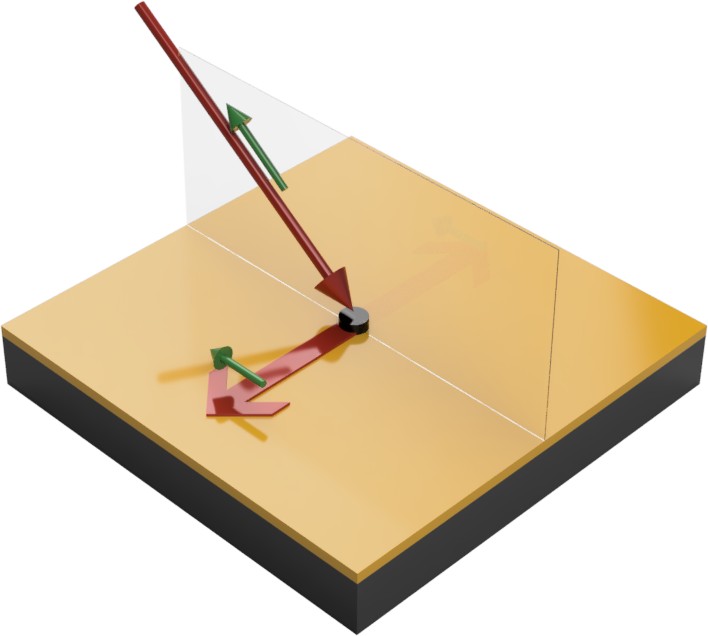
\includegraphics[width=\textwidth]{figures/pshe_left.png}
			\caption{}
			\label{fig:pshe_left}
		\end{subfigure}		
		\begin{subfigure}[h]{0.5\textwidth}
			\centering
			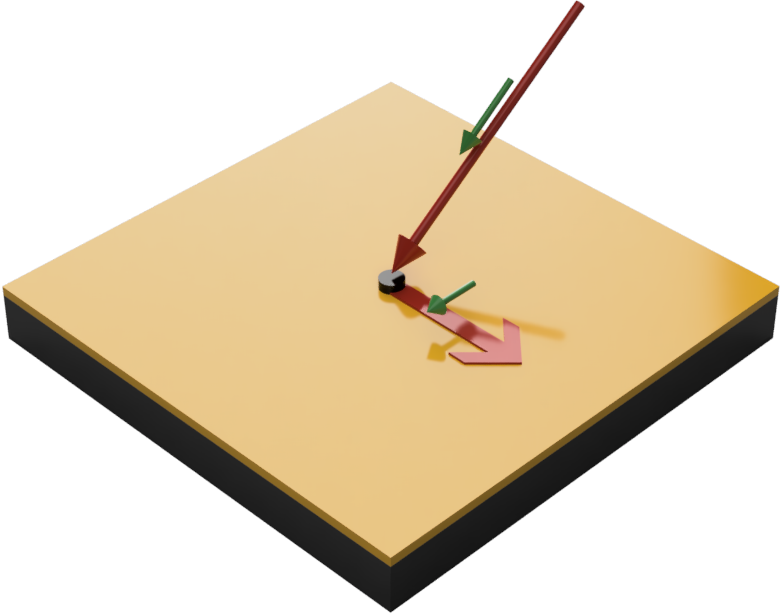
\includegraphics[width=\textwidth]{figures/pshe_right.png}
			\caption{}
			\label{fig:pshe_right}
		\end{subfigure}	
		\caption[Drehimpuls-Erhaltung beim PSHE]{Drehimpulserhaltung-Erhaltung beim PSHE. Der schräge Pfeil veranschaulicht die anregende EM-Strahlung. Der Pfeil auf der Goldoberfläche stellt die Propagationsrichtung des SPP da. In grün ist jeweils der Drehimpuls des SPP und der anregenden Strahlung gekennzeichnet. Die Einfallsebene ist durch eine transparente Fläche gekennzeichnet.}
		\label{fig:spin_hall_schema}
	\end{figure}	
	\section{Messmethoden und experimenteller Aufbau}
	\subsection{Einstellung der Polarisation des Lasers}
	\label{sec:cntr_pol}
	Um den optischen Spin-Hall-Effekt nachweisen zu können, ist es notwendig, die Polarisation des Anregungslasers zu kontrollieren. Hierfür wurden ein Polarisationsfilter und eine $\lambda /4$-Verzögerungsplatte verwendet. Der in dieser Arbeit verwendete He-Ne-Laser der Firma \textit{Thorlabs} ist annähernd linear polarisiert.
	\subsubsection{Bestimmung der Polarisation des Anregungslasers}
	\label{sec:polarimeter}
	Für die Kontrolle der Polarisation des Anregungslasers ist es von entscheidender Bedeutung, dass der ursprüngliche Polarisationszustand bekannt ist. Außerdem zeigt die folgende Messung, dass die von den Herstellern angegebenen Orientierungen des $\lambda/4$-Plättchens und des Polarisationsfilters näherungsweise stimmen. Die Messungen sind außerdem ein starkes Indiz dafür, dass sowohl das $\lambda/4$-Plättchen als auch der Polarisationsfilter ordnungsgemäß funktionieren. Die folgenden Ausführungen sind für das Verständnis der weiteren Arbeit nicht zwingend erforderlich, schließen aber einige wichtige Fehlerquellen aus. Außerdem zeigt die folgende Messung, dass der Polarisationsfilter, der in dem Hauptaufbau vor dem $\lambda / 4$-Plättchen verwendet worden ist, um die Polarisation vor dem $\lambda / 4$-Plättchen zu definieren, notwendig ist. Der Quellcode für die in diesem Abschnitt durchgeführte Simulation ist unter \url{https://github.com/hanno22/SpinHallEffectThesis/blob/master/models} in den Dateien \textit{JonesFormalism.py} und \textit{Lambda4OrientationDataSet.py} zu finden. (Die Funktionalität ist dort jeweils in Klassen gegliedert.)
	\paragraph{Jones-Formalismus}
	Der Jones-Formalismus ist ein Verfahren, welches es ermöglicht, die Polarisation von elektromagnetischer Strahlung mathematisch zu beschreiben. Die folgenden Ausführungen orientieren sich an \cite{Hecht.2018}. Das elektrische Feld einer monochromatischen ebenen Welle mit der Kreisfrequenz $\omega$ und der Wellenzahl $k$ die entlang der $z$-Richtung propagiert lässt sich durch folgenden Ausdruck beschreiben:
	\begin{equation}
		\vec{E}(z, t) = \underbrace{\begin{pmatrix}E_x \\ E_y\end{pmatrix}}_{\vec{J}} \exp(i(kz-\omega t))
	\end{equation}
	Hierbei ist $\vec{J} := \begin{pmatrix}E_x \\ E_y\end{pmatrix}$ der aus den beiden komplexen Zahlen $E_x, E_y$ bestehende Jones-Vektor. Der Jones-Vektor beschreibt also die Amplitude und das Phasenverhältnis der beiden Feldkomponenten und charakterisiert den Polarisationszustand der EM-Welle somit vollumfänglich. Der Jones-Vektor wird folglich durch die vier reellen Parameter $\Re\{E_x\}, \Im\{E_x\}, \Re\{E_y\}, \Im\{E_y\}$ vollständig bestimmt. Es gibt neben diesem Parametersatz auch noch weitere Kombinationen von vier Parametern, die den Polarisationzustand umfassend beschreiben. Der Übergang in einen anderen Parametersatz entspricht einem Basiswechsel des Jones-Vektors.	Ein beliebiges optisches Element, dass den Polarisationzustand einer EM-Welle beinflusst, lässt sich nun durch eine komplexe $2 \times 2$-Jones-Matrix $\boldsymbol{M}$ beschreiben. Wenn die EM-Welle vor dem optischen Element den durch den Jones-Vektor $\vec{J}$ beschriebenen Polarisationszustand hat, besitzt sie nach dem Durchgang durch das optische Element den Polarisationszustand $\vec{J}^\prime$, der sich durch folgenden Ausdruck berechnen lässt:
	\begin{equation}
		\vec{J}^\prime = \boldsymbol{M} \vec{J}  =  
		\begin{pmatrix}
			M_{11} & M_{12} \\
			M_{21} & M_{22}
		\end{pmatrix}
		\begin{pmatrix}
			J_x \\
			J_y
		\end{pmatrix} = 
		\begin{pmatrix}
			M_{11} J_x + M_{12} J_y \\
			M_{21} J_x + M_{22} J_y
		\end{pmatrix}		
	\end{equation}
	Unterschiedliche optische Elemente lassen sich durch verschiedene Jones-Matrizen beschreiben. So ist die Jones-Matrix eines in $x$-Richtung orientierten Polarisationsfilters beispielsweise:
	\begin{equation}
		\boldsymbol{M}_{\mathrm{PF}} = \begin{pmatrix}
			1 & 0 \\
			0 & 0
		\end{pmatrix}
	\end{equation}
	oder eines $\lambda/4$-Plättchens, bei dem die schnelle Achse entlang der $x$-Richtung orientiert ist:	
	\begin{equation}
		\boldsymbol{M}_{\mathrm{\lambda / 4}} = \dfrac{1}{\sqrt{2}}\begin{pmatrix}
			1-i & 0 \\
			0 & 1+i
		\end{pmatrix}
	\end{equation}
	Die Drehung eines optischen Elements lässt sich durch die Anwendung einer Rotationsmatrix auf die Jones-Matrix ausdrücken:
	\begin{equation}
		\boldsymbol{M}(\Phi) = \boldsymbol{R}(\Phi)\boldsymbol{M}\boldsymbol{R}(-\Phi)
	\end{equation}
	mit der Rotationsmatrix:
	\begin{equation}
		\boldsymbol{R}(\Phi) = \begin{pmatrix}
			\cos\Phi & - \sin\Phi \\
			\sin\Phi & \cos\Phi
		\end{pmatrix}
	\end{equation}
	\paragraph{Bestimmung der Polarisation des Anregungslasers mit Hilfe eines Jones-Polarimeters}
	Ein Polarimeter ist eine Apparatur, die eine vollständige Bestimmung der Polarisation einer EM-Welle ermöglicht. Eine Realisierung eines Polarimeters ist ein Jones-Polarimeter. Dieses besteht in Strahlreihenfolge aus einem $\lambda / 4$ Plättchen, einem Polarisationsfilter und einem Leistungsmessgerät (Abbildung \ref{fig:polarimeter}). Um den Jones-Vektor $\vec{J}$ einer monochromatischen ebenen Welle mit Hilfe des Jones-Polarimeters zu bestimmen, wird die Leistung in Abhängigkeit der Orientierung $\alpha_{\lambda/4}$ des $\lambda / 4$-Plättchens gemessen: $P = P(\alpha_{\lambda/4})$. Die Form dieses Leistungsverlaufes hängt nur von dem ursprünglichen Polarisationszustand der EM-Strahlung ab. Um aus $P(\alpha_{\lambda/4})$ die Komponenten des Jones-Vektor $\vec{J}$ zu rekonstruieren, wurde das Experiment mit einem \textit{Python}-Skript simuliert. Der Polarisationszustand hinter dem Polarimeter $\vec{J}^\prime$ lässt sich mit Hilfe des Jones-Formalismus durch folgenden Ausdruck berechnen:
	\begin{equation}
		\vec{J}^\prime = \boldsymbol{M}_\mathrm{PF} \boldsymbol{R}(\alpha_{\lambda/4})\boldsymbol{M}_{\lambda / 4}\ \boldsymbol{R}(-\alpha_{\lambda/4})\vec{J}
	\end{equation}
	Die Intensität und damit auch die Leistung bei konstantem Strahlquerschnitt, die das Leistungsmessgerät erreicht, ist hierbei proportional zum Betragsquadrat des Jones-Vektors:
	\begin{equation}
		P(\vec{J}^\prime) \propto \left|\vec{J}^\prime\right|^2
	\end{equation}
	Die theoretisch errechnete Leistung $P$, die an dem Leistungsmessgerät erwartet wird, ergibt sich also in Abhängigkeit von $\alpha_{\lambda/4}$ und $\vec{J}$ zu:
	\begin{equation}
		P(\alpha_{\lambda/4}, \vec{J}) = \left|\boldsymbol{M}_\mathrm{PF} \boldsymbol{R}(\alpha_{\lambda/4})\boldsymbol{M}_{\lambda / 4}\ \boldsymbol{R}(-\alpha_{\lambda/4})\vec{J}\right|^2 \cdot \mathrm{const.}
		\label{eq:simulation_polarimeter}
	\end{equation}
	Diese Funktion kann nun mit den Komponenten von $\vec{J}$ als Parameter mit Hilfe der Methode der kleinsten quadratischen Abweichung (engl. \textit{least square fit}) an die Messdaten angepasst werden. Die resultierenden Fit-Parameter sind dann die Komponenten des ursprünglichen Jones-Vektors $\vec{J}$. Dieser Fit an die Messdaten und die aus $\vec{J}$ resultierende Polarisations-Ellipse sind in Abbildung \ref{fig:graphpolarimeter} dargestellt. In der Abbildung ist zu erkennen, dass die Messdaten sehr gut mit der Simulation übereinstimmen. Dies ist ein starkes Indiz für die korrekte Funktionsweise der Komponenten. Allerdings zeigt die Messung auch, dass der Laser nicht rein linear polarisiert ist. Ein Maß für die Abweichung von der linearen Polarisation ist die Elliptizität $\epsilon$ der Polarisation:
	\begin{equation}
		\epsilon = \dfrac{a}{b}
	\end{equation}
	Hierbei ist $a$ die große und $b$ die kleine Halbachse der Polarisationsellipse. Die Elliptizität des Lasers wurde in dieser Arbeit durch den Fit der Simulation auf $\epsilon = 0.1 $ bestimmt. Durch diese Abweichungen des Lasers von einer rein linearen Polarisation war es notwendig, die Polarisation des Lasers vor dem $\lambda /4$-Plättchen im Hauptaufbau durch einen Polarisationsfilter festzulegen.
	\begin{figure}
		\centering
		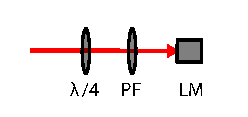
\includegraphics[width=0.5\linewidth]{figures/Polarimeter}
		\caption[Jones-Polarimeter]{Die Abbildung zeigt den schematischen Aufbau eines Jones-Polarimeter. Die Komponenten in Strahlreihenfolge sind: Helium-Neon-Laser (\textbf{He-Ne}), $\lambda/4$-Plättchen ($\boldsymbol{\lambda / 4}$), Polarisationsfilter (\textbf{PF}), Leistungsmessgerät(\textbf{LM}). Das $\lambda/4$-Plättchen kann um die optische Achse rotiert werden.}
		\label{fig:polarimeter}
	\end{figure}
	\begin{figure}
		\centering
		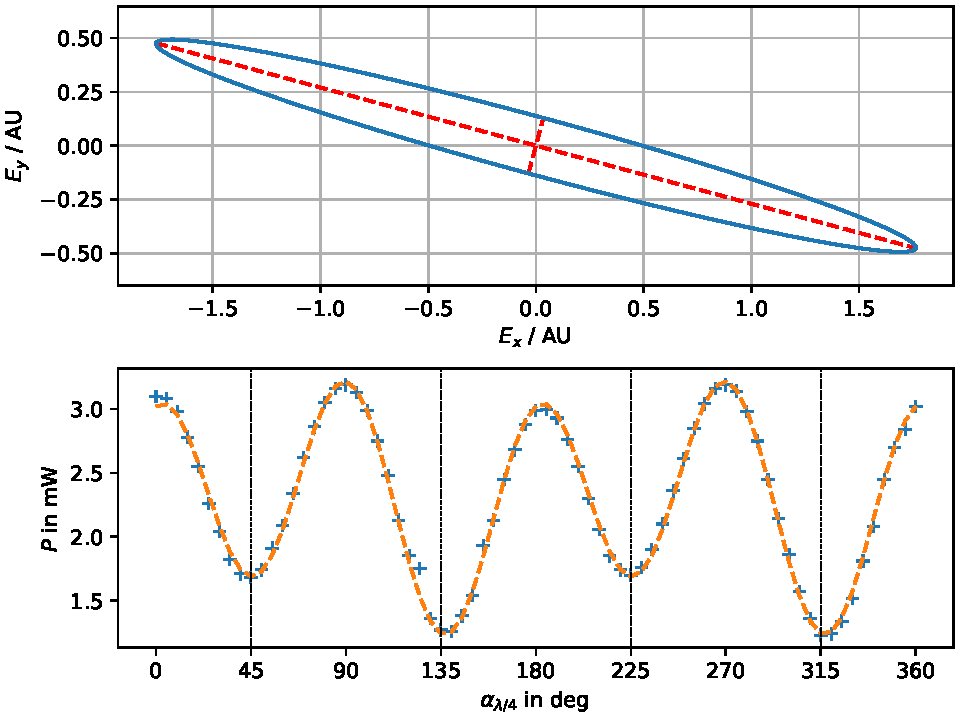
\includegraphics[width=0.7\linewidth]{figures/graph_polarimeter}
		\caption[Polarimeter Simulation]{Diese Abbildung zeigt die Daten einer Messung mit dem Jones-Polarimeter. Der untere Teil der Abbildung zeigt die gemessene Leistung $P(\alpha_{\lambda /4})$. Die blauen Kreuze sind hierbei jeweils Messpunkte. Die orange gestrichelte Linie zeigt die mit einem \textit{least square fit} an die Messdaten angepasste Simulation des Polarimeteraufbaus. Der obere Teil der Abbildung zeigt die im unteren Teil verwendeten Fit-Parameter für den Jones-Vector $\vec{J}$. Hierbei wurden die Polarisationsellipse sowie die zwei Halbachsen $a$ und $b$ eingezeichnet. Die Feldstärken sind dabei in willkürlichen Einheiten dargestellt, da für die exakte Feldstärkenbestimmung nicht die Leistung, sondern die Intensität nach dem Durchgang durch das Polarimeter gemessen werden müsste.}
		\label{fig:graphpolarimeter}
	\end{figure}
	\subsubsection{Polarisationsfilter}	
	Um den Polarisationszustand des Lasers präzise festzulegen, wurde ein linearer Polarisationsfilter verwendet. Ein beliebiger Polarisationszustand lässt sich immer durch eine Überlagerung von zwei senkrecht aufeinander stehenden linearen Polarisationen ausdrücken. Ein Polarisationsfilter transmittiert nur Licht, welches entlang einer festgelegten Achse linear polarisiert ist. Die anderen Polarisationsrichtungen werden absorbiert oder reflektiert. Ein Polarisationsfilter kann also aus einer beliebigen Polarisation linear polarisiertes Licht erzeugen. Der  Polarisationsfilter wurde nach dem letzten Spiegel des optischen Aufbaus positioniert, da ein Spiegel im Allgemeinen unterschiedliche Reflektivitäten für EM-Strahlung aufweist, je nachdem, ob diese Strahlung senkrecht oder vielmehr parallel zur Einfallsebene des Strahls auf den Spiegel polarisiert ist. Der Filter wurde auf eine Polarisation parallel zur Einfallsebene eingestellt und der Laser dann so entlang der optischen Achse verdreht, dass die gemessene Leistung hinter dem Polarisationsfilter maximal ist. So entsteht hinter dem Polarisationsfilter unabhängig  von der exakten ursprünglichen Polarisation des Lasers $p$-polarisiertes Licht, ohne dabei zu große Leistungsverluste an dem Polarisationsfilter zu erzeugen.\cite{Hecht.2018}
	\subsubsection{Verzögerungsplättchen}
	Mit einem Verzögerungsplättchen lässt sich die Polarisation einer einfallenden Welle verändern. Eine EM-Welle lässt sich immer als Überlagerung von zwei linear und senkrecht zueinander polarisierten Wellen beschreiben. Diese beiden senkrecht aufeinander stehenden Polarisationen sind im Allgemeinen zueinander phasenverschoben. Das Funktionsprinzip eines Verzögerungsplättchens besteht darin, die relative Phasenverschiebung zwischen diesen beiden Polarisationen zu verändern. So kann man mit einem geschickt gewählten Verzögerungsplättchen aus jeder beliebigen Ausgangspolarisation in einen beliebigen anderen Polarisationszustand wechseln. Ein Verzögerungsplättchen weist immer eine schnelle und eine langsame Achse auf. Diese beiden Achsen stehen senkrecht aufeinander. Die Phasenverschiebung $\Delta\Phi$ zwischen zwei EM-Wellen, von denen die eine entlang der langsamen Achse und die andere entlang der schnellen Achse linear polarisiert ist, stellt eine charakteristische Größe des jeweiligen Verzögerungsplättchens dar. Physikalisch  werden Verzögerungsplättchen durch doppelbrechende Kristalle realisiert. Die jeweilige Phasendifferenz ist hierbei von der Dicke des doppelbrechenden Kristalls und von den Brechungsindizes der langsamen und der schnellen Kristallachse abhängig. Wenn diese Größen so dimensioniert sind, dass die Phasendifferenz zwischen den beiden Polarisationen, die eine EM-Welle beim Durchgang durch das Plättchen erfährt, $\Delta \Phi = \pi /4 $ ist, spricht man von einem  $\lambda /4$-Verzögerungsplättchen. Diese Phasendifferenz ist immer an eine bestimmte Wellenlänge angepasst.  Ein $\lambda /4$-Verzögerungsplättchen kann aus linear polarisiertem Licht zirkular polarisiertes Licht erzeugen, wenn eine der beiden Kristallachsen eine Orientierung von 45° zur ursprünglichen Polarisationsachse des Lasers aufweist \cite{Hecht.2018}. Diese Eigenschaft wurde in dieser Arbeit ausgenutzt. In Abbildung \ref{fig:polarisationlambda} ist die Polarisation hinter dem Verzögerungsplättchen in Abhängigkeit der relativen Orientierung vom Polarisationsfilter zum $\lambda /4$-Verzögerungsplättchen dargestellt. 
	\begin{figure}[h]
		\begin{subfigure}[h]{0.49\textwidth}
			\centering
			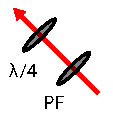
\includegraphics[width=0.5\textwidth]{figures/polarisation_control.pdf}
			\caption{}
			\label{fig:pol_control_scheme}
		\end{subfigure}
		%\hfill	
		\begin{subfigure}[h]{0.5\textwidth}
			\centering
			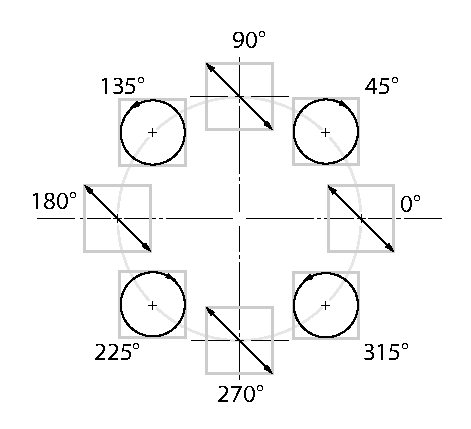
\includegraphics[width=\textwidth]{figures/Polarisation_lambda}
			\caption{}
			\label{fig:polarisationlambda}
		\end{subfigure}	
		\caption[Polarisation $\lambda/4$-Plättchen]{Abbildung \subref{fig:pol_control_scheme} zeigt die zur Kontrolle der Polarisation der anregenden Strahlung verwendete Konfiguration aus Polarisationsfilter (PF) und $\lambda/4$-Plättchen ($\lambda/4$). Abbildung \ref{fig:polarisationlambda} zeigt die Polarisation hinter dem $\lambda/4$-Plättchen in Abhängigkeit von der relativen Orientierung zwischen $\lambda/4$-Plättchen und Polarisationsfilter.}
		\label{fig:pol_control}
	\end{figure}

	\subsection{Leckstrahlmikroskopie}
	In dieser Arbeit kommt ein Leckstrahlmikroskop (LRM) zum Einsatz, um den PSHE experimentell nachzuweisen. Ein LRM hat gegenüber anderen Methoden zur Untersuchung plasmonischer Systeme den Vorteil, dass es rein optisch arbeitet und deswegen nicht auf aufwendige Vakuum-Technik angewiesen ist. Ein LRM nutzt aus, dass ein SPP in einem Mehrschichtsystem, wie in Abschnitt \ref{sec:leakage_radiation} erläutert, Leckstrahlung unter einem spezifischen Winkel in ein Substrat dissipiert. Als Probe wurde in dieser Arbeit ein auf ein Glassubstrat aufgedampfter Goldfilm verwendet. Das Schichtsystem besteht also aus der Abfolge Luft-Gold-Glas.
	
	Ein Defekt auf der Probe wird zunächst von der Luftseite mit einem Laser bestrahlt. An der Luft-Gold-Grenzfläche werden hierdurch SPPs angeregt. Diese SPPs geben nun Leckstrahlung in das Glassubstrat ab.
	Außerdem wird ein Teil des Lasers direkt transmittiert. Auf der Glasseite der Probe werden mit einem Immersionsobjektiv die Leckstrahlung und der direkt transmittierte Laser gesammelt und abgebildet.	
	Aus diesem Bild wird mit Hilfe eines 4f-Aufbaus (Abschnitt \ref{sec:fourier}) die Leckstrahlung selektiert, welche unter dem spezifischen Leckstrahlwinkel aus dem Glassubstrat ausgetreten ist. So ist es möglich, die plasmonischen Anregungen ohne Störungen des direkt transmittierten Strahls zu beobachten. Das in dieser Arbeit verwendete LRM basiert auf dem Aufbau, den \textit{Jaruschewski} im Rahmen seiner Masterarbeit \cite{Jaruschewski.2020} entwickelt hat.
	\subsubsection{Immersionsobjektiv}
	Da der Winkel, unter dem das SPP Leckstrahlung in das Glas abgibt, größer ist als der kritische Winkel für die Totalreflexion an der Grenzschicht Glas-Luft, muss für die Abbildung der Leckstrahlung ein Immersionsobjektiv verwendet werden. Ein Immersionsobjektiv nutzt ein Immersionsöl, das zwischen Objektiv und Probe aufgebracht wird. Durch die Adhäsions- und Kohäsionskräfte in dem Öl ist es möglich, dauerhaft einen kleinen Öltropfen zwischen Objektiv und Probe zu halten. In dieser Arbeit  wurde eine sogenannte homogene Immersion verwendet, dies bedeutet, dass die Brechungsindices von Deckglas, Immersionsöl und Frontlinse des Immersionsobjektives sehr nah beieinander liegen. Dadurch tritt an der Grenzfläche Glas-Immersionsöl für die Leckstrahlung keine Totalreflexion auf. Durch den großen Winkel, unter dem die Leckstrahlung aus der Probe austritt, ist es außerdem notwendig, dass das Objektiv einen großen maximalen Öffnungswinkel aufweist, damit die Leckstrahlung korrekt abgebildet und nicht im Inneren des Objektives absorbiert wird. Die Fähigkeit eines Objektivs, Licht unter großen Winkeln zur optischen Achse aufzunehmen, lässt sich durch die numerische Apertur $\mathrm{NA} = n\sin\theta_{max}$ beschreiben. $n$ ist hierbei der Brechungsindex des Mediums vor dem Objektiv, und $\theta_{max}$ ist der halbe maximale Öffnungswinkel des Objektivs. Die numerische Apertur berücksichtigt also, dass der Winkel eines Strahls zur optischen Achse durch Verwendung eines Mediums mit großem Brechungsindex zwischen Objektiv und Probe verkleinert werden kann. Eine große numerische Apertur bedeutet, dass das Objektiv Licht auch noch unter großen Winkeln zur optischen Achse aufnehmen kann. In dieser Arbeit wurde ein Immersionsöl mit Brechungsindex $n_{"ol} = 1.518$ und ein Immersionsobjektiv mit $\mathrm{NA} = 1.216$ verwendet. Hieraus ergibt sich ein maximaler halber Öffnungswinkel von $\theta_{max} = \arcsin(\mathrm{NA} / n_{"ol}) = 53.2^\circ > \theta_L = 43.2^\circ$. Das verwendete Immersionsobjektiv kann die Leckstrahlung, die unter dem Winkel $\theta_L = 43.2^\circ$ \eqref{eq:theo_theta_l} aus der Probe austritt, also abbilden. Ferner ist das Immersionsobjektiv unendlich korrigiert. Dies bedeutet, dass die Korrekturen der Abbildungsfehler des Objektivs darauf abgestimmt worden sind, dass die Probe in der Brennweite des Objektivs steht. Wenn die Probe in der Brennweite des Objektivs steht, ist die Strahlung, welche aus dem Objektiv austritt, parallel und das Zwischenbild entsteht erst im Unendlichen. (Unter Vernachlässigung der komplexen Abbildungskorrekturen kann ein Objektiv als eine einfache Sammellinse angesehen werden.) Um dieses Zwischenbild in eine endliche Distanz zu verschieben, ist noch eine weitere Sammellinse, die Tubuslinse notwendig. Ein unendlich korrigiertes Objektiv kann auch außerhalb dieser Betriebsart verwendet werden. Allerdings treten dann zunehmend Fehler in der Abbildung auf. Der korrekte Betrieb des Objektivs kann durch die Position des Zwischenbildes hinter der Tubuslinse überprüft werden. Liegt das Zwischenbild hinter der Tubuslinse genau in deren Brennweite, so liegt die Probe in der Brennweite des Objektivs und die Abbildung des Objektives ist optimal korrigiert.\cite{Kuhl.2018} Der Strahlengang für zwei Sammellinsen unterschiedlicher Brennweite in der unendliche korrigierten Betriebsart ist in Abbildung \ref{fig:bildentstehungobjektiv} dargestellt.
	\begin{figure}
		\centering
		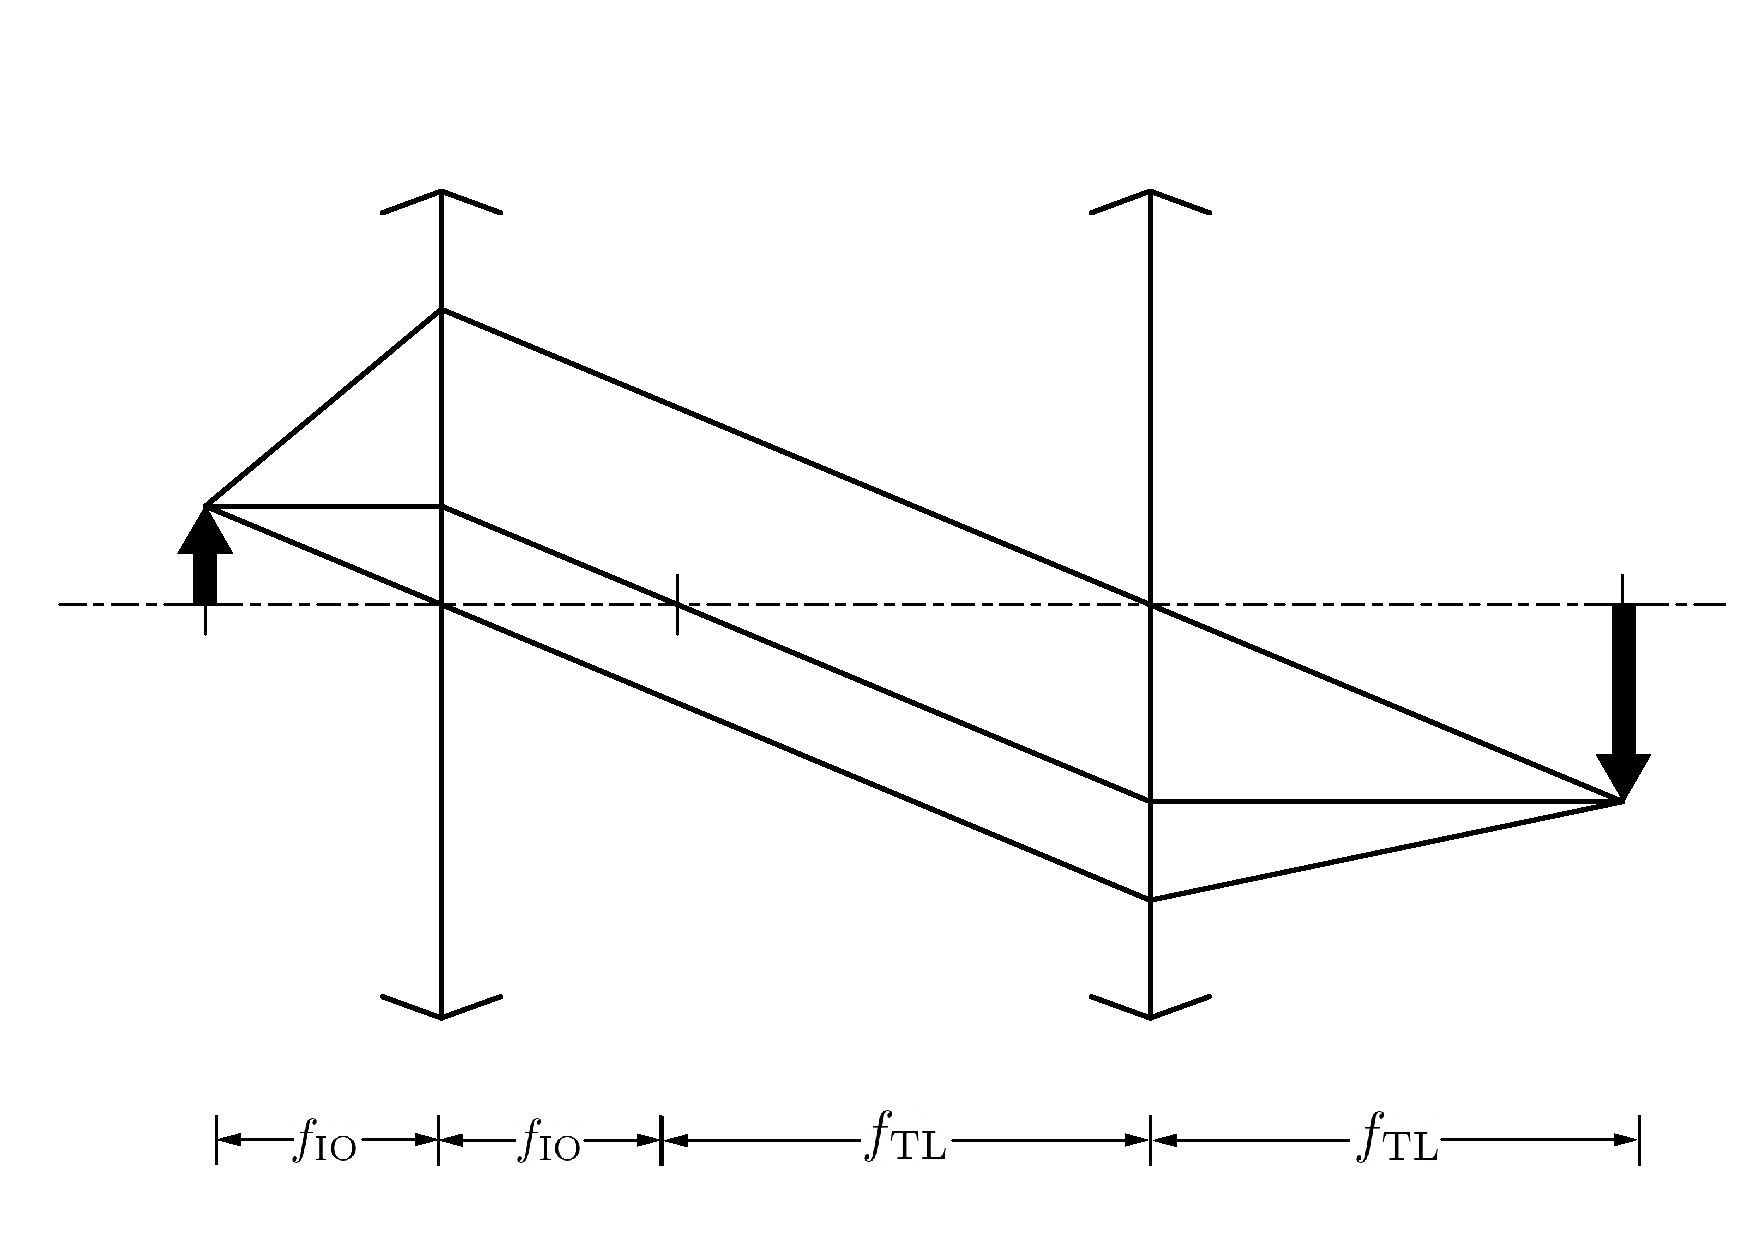
\includegraphics[width=0.7\linewidth]{figures/BildentstehungObjektiv.pdf}
		\caption[Strahlengang unendlich korrigiertes Objektiv]{Die Abbildung zeigt den Strahlengang für zwei Sammellinsen. Die erste Sammellinse imitiert dabei das Immersionsobjektiv mit der Brennweite $f_\mathrm{IO}$ und die zweite Sammellinse imitiert die Tubuslinse mit der Brennweite $f_\mathrm{IO}$. Das Immersionsobjektiv wird in der 'unendliche korrigierten' Betriebsart verwendet. Das Objekt befindet sich also in der Brennweite $f_\mathrm{IO}$ des Immersionsobjektives. Der Abstand zwischen den beiden Sammellinsen beträgt in der Abbildung gerade $f_\mathrm{IO} + f_\mathrm{TL}$, kann aber frei gewählt werden, da die Strahlen zwischen den Linsen parallel verlaufen. Das vergrößerte Bild des Objektes entsteht in der hinteren Brennebene der Tubuslinse.}
		\label{fig:bildentstehungobjektiv}
	\end{figure}
	
	\subsubsection{Fourier-Optik}
	\label{sec:fourier}
	\begin{figure}[htbp] 
		\centering
		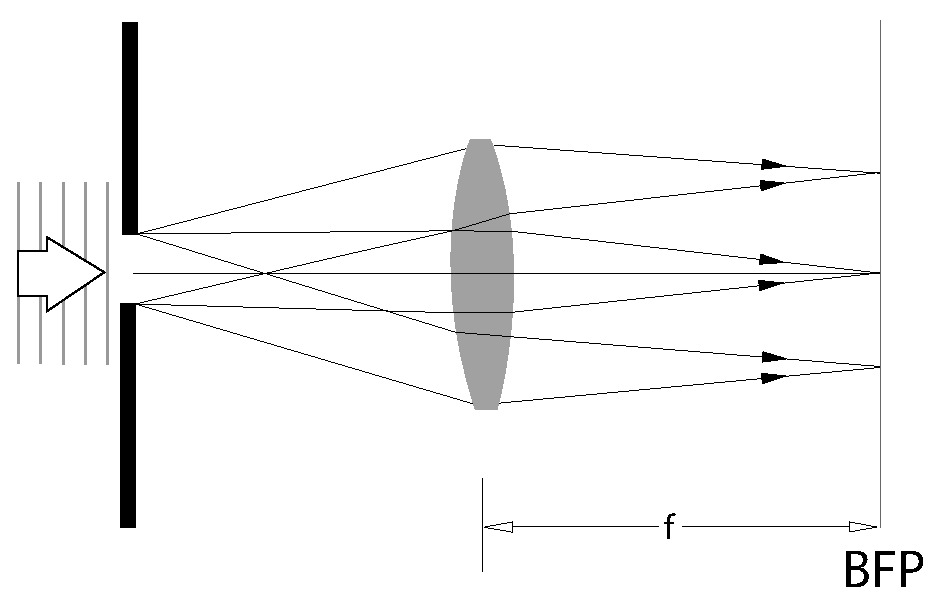
\includegraphics[width=0.5\textwidth]{figures/FourierLinse.pdf}
		\caption[Fourieroptik]{Eine Sammellinse erzeugt das Fraunhofersche Beugungsbild in ihrer hinteren Brennebene (BFP). Parallele Strahlen werden in Abhängigkeit ihres Winkels zur optischen Achse auf einem Punkt in der BFP fokussiert. Die Abbildung ist an eine Abbildung aus \cite{Hecht.2018} angelehnt.}
		\label{fig:FourierLinse}
	\end{figure}
	Da hinter der Probe nicht nur die Leckstrahlung, sondern auch die Strahlung des direkt transmittierten Strahls zu beobachten ist, ist es notwendig, die Leckstrahlung zu selektieren. Die Leckstrahlung tritt dank der notwendigen Phasenanpassung nur unter einem charakteristischen Winkel zur optischen Achse \eqref{eq:phase_condition} aus der Probe aus. Daher ist es möglich, die Leckstrahlung durch ihren Emissionswinkel zu identifizieren. Hierfür ist die Fourier-Optik nützlich. Eine Sammellinse besitzt die Eigenschaft, in  der hinteren Brennebene (eng. Back Focal Plane BFP) ein winkelaufgelöstes Bild von der Strahlung, die sie erreicht, zu erzeugen\cite{Hecht.1996}. Die Position eines Lichtstrahls in der BFP ist also nur von dem Winkel des Strahls zur optischen Achse, nicht aber von der absoluten Position des Strahls vor der Linse abhängig. So ist es möglich, gezielt bestimmte Emissionswinkel in der BFP aus dem Bild herauszufiltern. Dieses winkelaufgelöste Bild kann auch als eine räumliche Fouriertransformation der Feldstärkeverteilung an der beobachteten Struktur aufgefasst werden. 
	
	\paragraph{4f-Aufbau}
	In dieser Arbeit wird für diese optische Filterung ein $4f$-Aufbau verwendet. Ein $4f$-Aufbau besteht aus zwei Linsen mit der Brennweite $f$, die im Abstand $2f$ zueinander angeordnet werden. Die beiden Linsen werden so positioniert, dass sich im Abstand $f$ von der ersten Linse das Zwischenbild des Immersionsobjektivs befindet. Zwischen den beiden Linsen entsteht nun ein winkelaufgelöstes Fourierbild; Dieses wird durch die numerische Apertur des Immersionsbildes scharf begrenzt.  In diesem winkelaufgelösten Fourierbild kann nun gezielt ein Teil des Fourierspektrums (d.h. der Strahlung, die unter einem bestimmten Winkel zur optischen Achse aus der Probe ausgetreten ist) herausgefiltert werden. Die zweite Linse erzeugt nun aus diesem gefilterten Fourierspektrum wieder das Ortsbild. Dieses besteht nun nur noch aus den ausgewählten Fourierkomponenten. Der $4f$-Aufbau ist schematisch in Abbildung \ref{fig:aufbau_schema} erläutert. In dieser Arbeit wurde so der direkt transmittierte Strahl aus der optischen Abbildung eliminiert.
	\paragraph{Optionale Linse}
	Der $4f$-Aufbau erzeugt aus den ausgewählten Fourierkomponenten ein Ortsbild der Anregung. Da für die Analyse der Eigenschaften des SPP allerdings auch das winkelaufgelösten Fourierbild von Interesse ist, wurde hinter dem $4f$-Aufbau noch einen weitere optionale Linse aufgestellt. Diese wird genutzt, um das gefilterte Ortsbild in das gefilterte winkelaufgelöste Fourierbild zu transformieren. Die Linse kann leicht demontiert werden, um schnell zwischen den beiden Darstellungsarten zu wechseln. Die Winkelauflösung kann bei monochromatischer Strahlung auch als eine Darstellung der Komponenten des Wellenvektors die senkrecht auf der optischen Achse stehen aufgefasst werden. Da der Impuls eines Photons wiederum durch $p = \hbar k$ ausgedrückt werden kann, wird diese Darstellungsart auch als Impulsdarstellung bezeichnet.
	
	
	\subsection{Details des optischen Aufbaus}
	In dieser Arbeit wurde der Aufbau von \textit{Jaruschewski} \cite{Jaruschewski.2020} in einigen Details verbessert und umgerüstet, so dass der Laser auch unter schrägem Einfall auf die Probe gerichtet werden kann. Die verwendeten Komponenten sind detailliert in Anhang \ref{tab:components} aufgelistet. Der Aufbau ist in Abbildung \ref{fig:aufbau_schema} schematisch dargestellt. Als Anregungslaser wurde ein He-Ne-Dauerstrich-Laser der Firma \textit{Thorlabs} mit einer Leistung von $P = 35 \,\mathrm{mW}$ und einer Wellenlänge von $\lambda = 633\,\mathrm{nm}$ verwendet.
	\begin{figure}
		\centering
		\begin{subfigure}[b]{0.9\textwidth}		
			\centering
			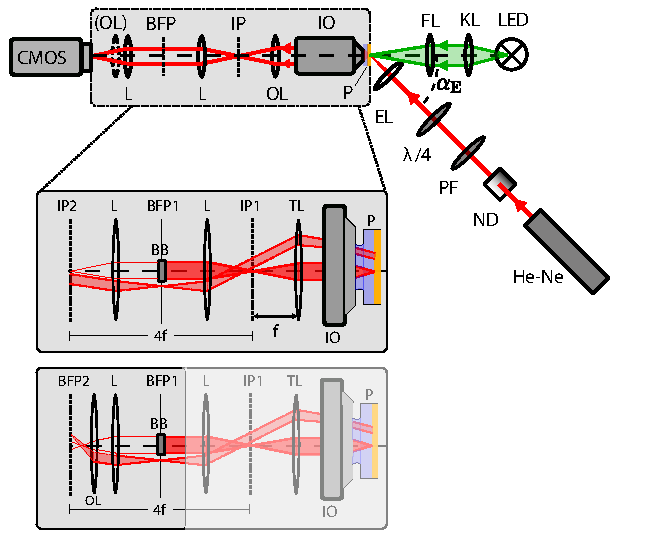
\includegraphics[width=0.9\textwidth]{figures/Aufbau_Schema.pdf}
			\caption{Schematischer Aufbau}			
			\label{fig:aufbau_schema}
		\end{subfigure}
		\vfil
		\begin{subfigure}[b]{0.9\textwidth} 
			\centering
			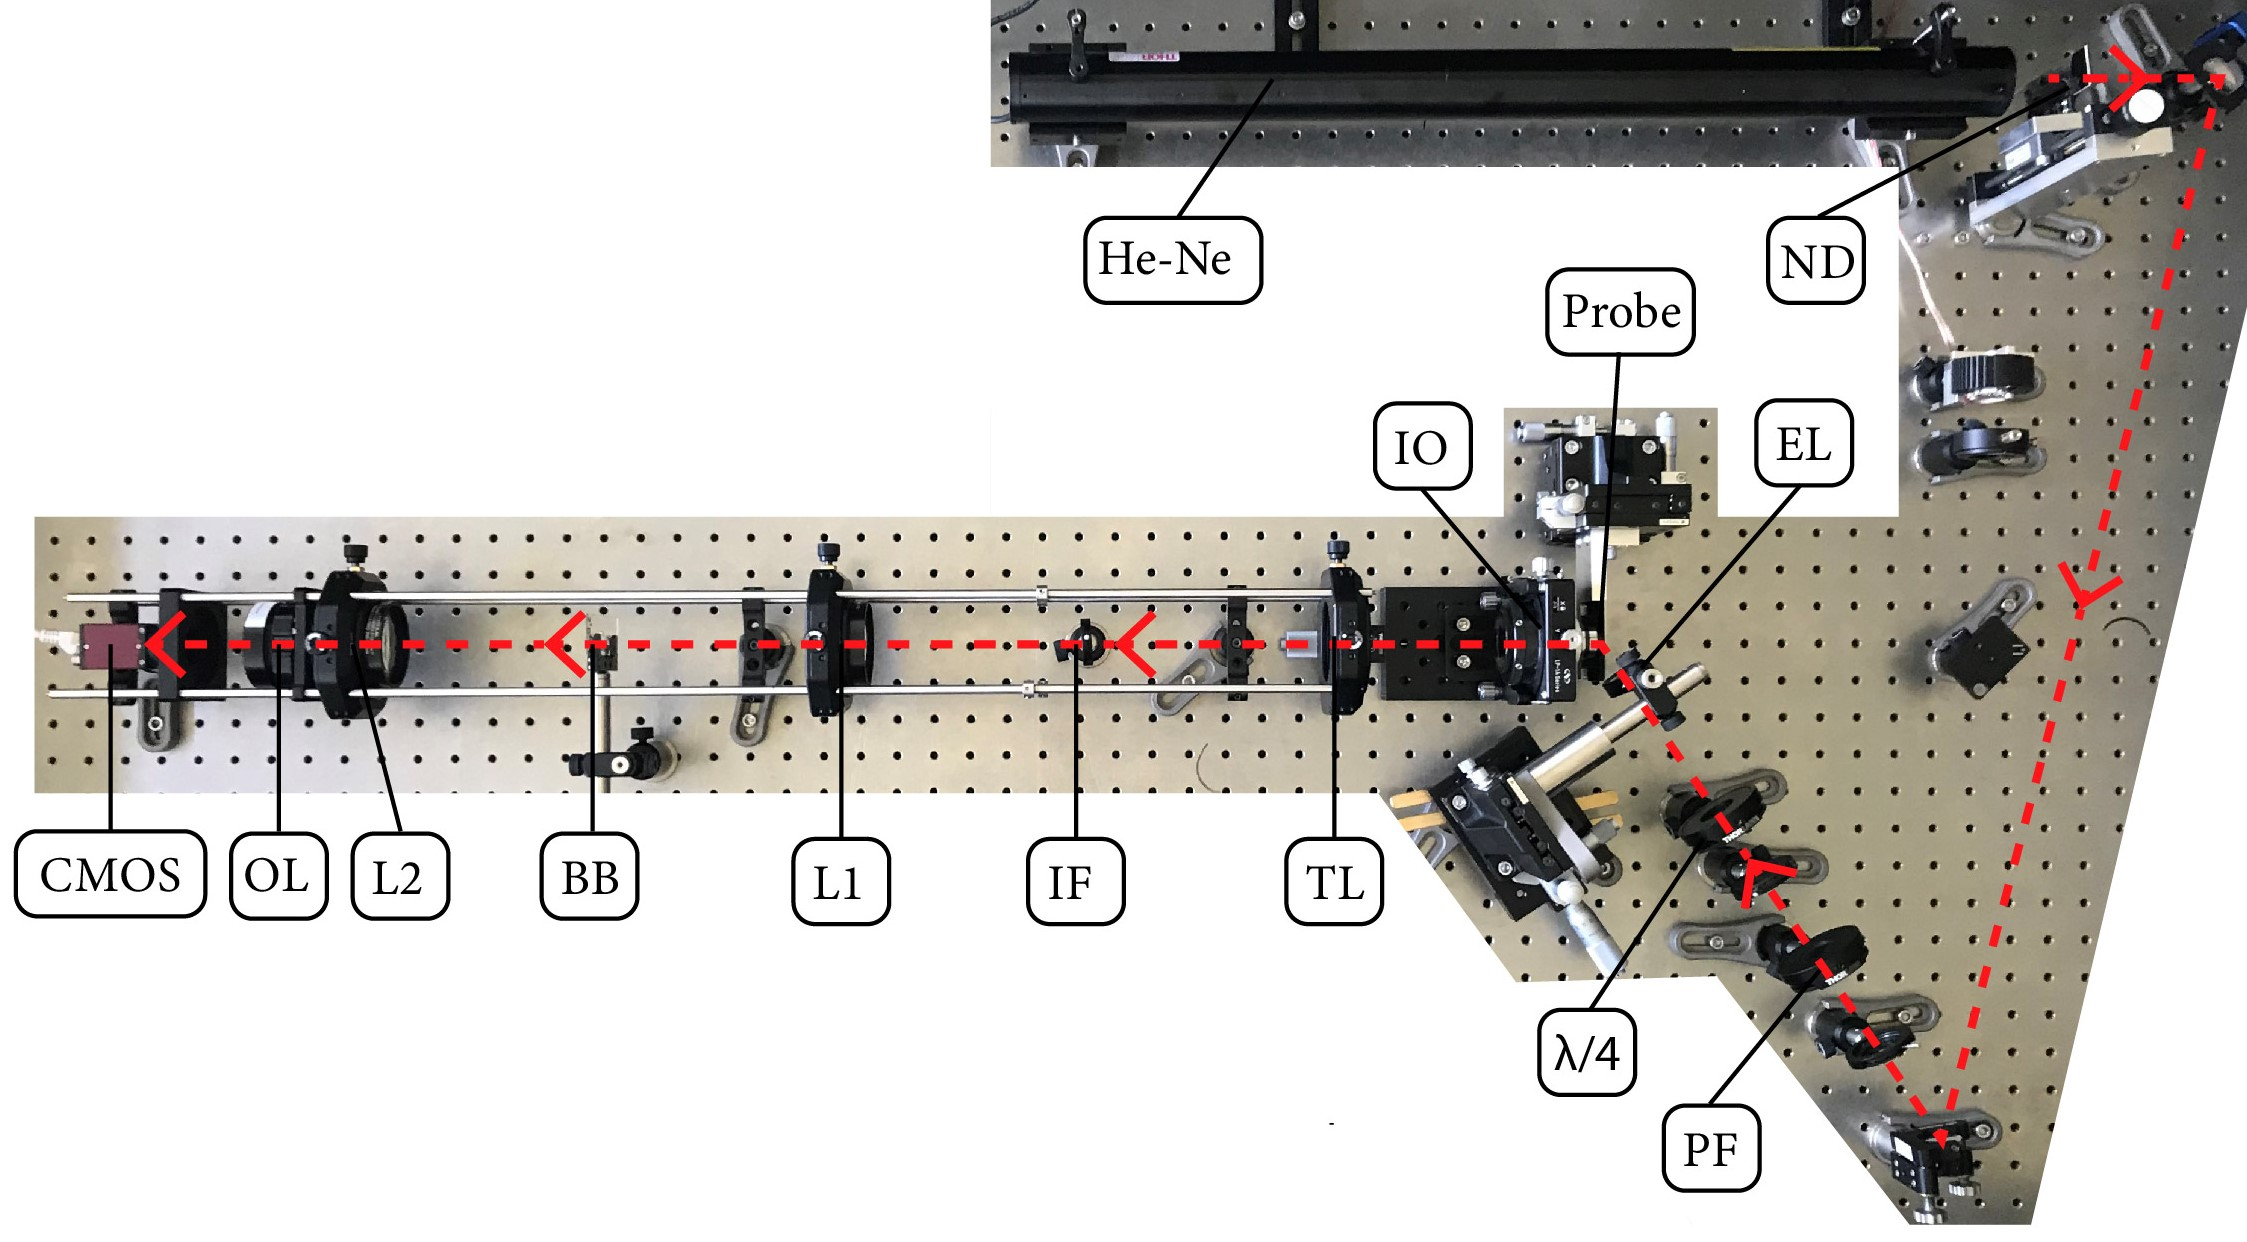
\includegraphics[width=0.9\textwidth]{figures/aufsicht_aufbau_anotated.jpg}
			\caption{Foto des Aufbau}
			\label{fig:aufsicht_aufbau_anotated}
		\end{subfigure}
		\caption[Versuchsaufbau]{Die Komponenten des Aufbaus sind: He-Ne-Laser (He-Ne), Neutraldichtefilter (ND), Polarisationsfilter (PF), Verzögerungsplättchen ($\lambda/4$), Einkoppel-Linse (EL), Probe (P), Immersionsobjektiv (IO), Linse 2 (L2), Image-Filter (IF), Linse 1 (L1), Beam-Block (BB), Linse 2 (L2), optionale Linse (OL), CMOS-Sensor (CMOS). Außerdem ist auch noch eine LED-Hintergrundbeleuchtung verbaut. In rot ist schematisch der Strahlengang des Lasers eingezeichnet. Die Abbildung des schematischen Aufbaus ist an eine Abbildung aus \cite{Jaruschewski.2020} angelehnt.}
		\label{fig:Aufbau}
	\end{figure}
	\subsubsection{Optische Komponenten und ihre Funktion}
		In diesem Abschnitt werden alle verwendeten optischen Komponenten benannt (in Strahlreihenfolge), und die zugehörige Funktion wird kurz erläutert. Die Komponenten sind in Abbildung \ref{fig:Aufbau} dargestellt.
		\begin{itemize}
			\item \textbf{Neutraldichtefilter (ND)} dient der Abschwächung des Lasers, um eine Überbelichtung des CMOS-Sensors zu verhindern.
			\item \textbf{Polarisationsfilter (PF)} dient der Kontrolle der Polarisation des Lasers (siehe Abschnitt \ref{sec:cntr_pol}).
			\item $\boldsymbol{\lambda / 4}$\textbf{-Plättchen (}$\boldsymbol{\lambda / 4}$\textbf{)} dient der Kontrolle der Polarisation des Lasers (siehe Abschnitt \ref{sec:cntr_pol}).
			\item \textbf{Einkoppellinse (EL)} dient der Fokussierung des Lasers auf die Probe, um hohe Intensitäten zu erreichen und möglichst gezielt einen Defekt zu beleuchten.
			\item \textbf{Probe (P)} Auf der Gold-Glas-Probe werden die SPP angeregt.
			\item \textbf{Immersionsobjektiv (IO)} dient der Abbildung der Leckstrahlung.
			\item \textbf{Tubuslinse (TL)} dient der Abbildung der Leckstrahlung.
			\item \textbf{Image-Block (IB)} dient der Filterung des Ortsbildes, so dass nur Leckstrahlung, die aus einem kleinen Bereich der Probe stammt, abgebildet wird.			
			\item \textbf{Linse 1 (L1)} ist Teil des 4f-Systems (siehe Abschnitt \ref{sec:fourier}).
			\item \textbf{Beam-Block (BB)} dient der Filterung der BFP. Der BB sperrt den direkt transmittierten Strahl.			
			\item \textbf{Linse 2 (L2)} ist Teil des 4f-Systems (siehe Abschnitt \ref{sec:fourier}).
			\item \textbf{Optionale Linse (OL)} kann aus dem Aufbau entfernt werden und wird verwendet, um zwischen orts- und impulsaufgelöstem Bild zu wechseln.
			\item \textbf{CMOS Sensor (CMOS)}  dient der Aufzeichnung des Bildes. Ist über Ethernet mit dem Computer verbunden.			
		\end{itemize}
		Um die Fokussierung der Probe zu erleichtern, wurde außerdem eine LED-Hintergrundbeleuchtung verwendet. Das Licht der LED wurde mit einer Sammellinse kollimiert und mit einer weiteren Linse FL $f_{\mathrm{FL}}=50\mathrm{mm}$ auf die  Probe fokussiert. Diese Linse wurde bei Bedarf mit einer Magnetsäule an der richtigen Stelle vor der Probe positioniert.
		
	\subsubsection{Veränderungen des vorhandenen Aufbaus}
	\paragraph{Einkoppellinse}
	Aus geometrischen Gründen war es nicht mehr möglich, den Laser mit einem Objektiv bei streifendem Einfall auf die Probe zu fokussieren, da sonst das Objektiv mit der Probe kollidieren würde. Stattdessen wurde eine Sammellinse als Einkoppellinse (EL) verwendet mit $f_{\mathrm{EL}}= 30\mathrm{mm}$. Die Wahl der Brennweite der Einkoppellinse ist ein Kompromiss: Je kleiner die Brennweite ist, desto kleiner lässt sich der Laser fokussieren. Wenn die Brennweite allerdings zu klein ist, kollidiert die Linsenhalterung mit der Probe. Mit kleinerer Brennweite sind also nur kleinere Einfallswinkel zur Probennormale möglich. Um trotzdem eine möglichst kleine Brennweite verwenden zu können, wurde eine sehr kompakte Linsenhalterung verwendet. Diese Halterung wurde über einen Querarm an einer xyz-Verfahreinheit montiert, so dass man die Linse in allen drei Raumrichtungen verfahren kann. Dies ist wichtig, um den Laser gezielt auf den Punkt zu fokussieren, an welchem die optische Achse die Probe schneidet. Dieser Aufbau ist in Abbildung \ref{fig:linsenhalterung} gezeigt.
	\begin{figure}
		\centering
		\begin{subfigure}[b]{0.4\textwidth}
			\centering
			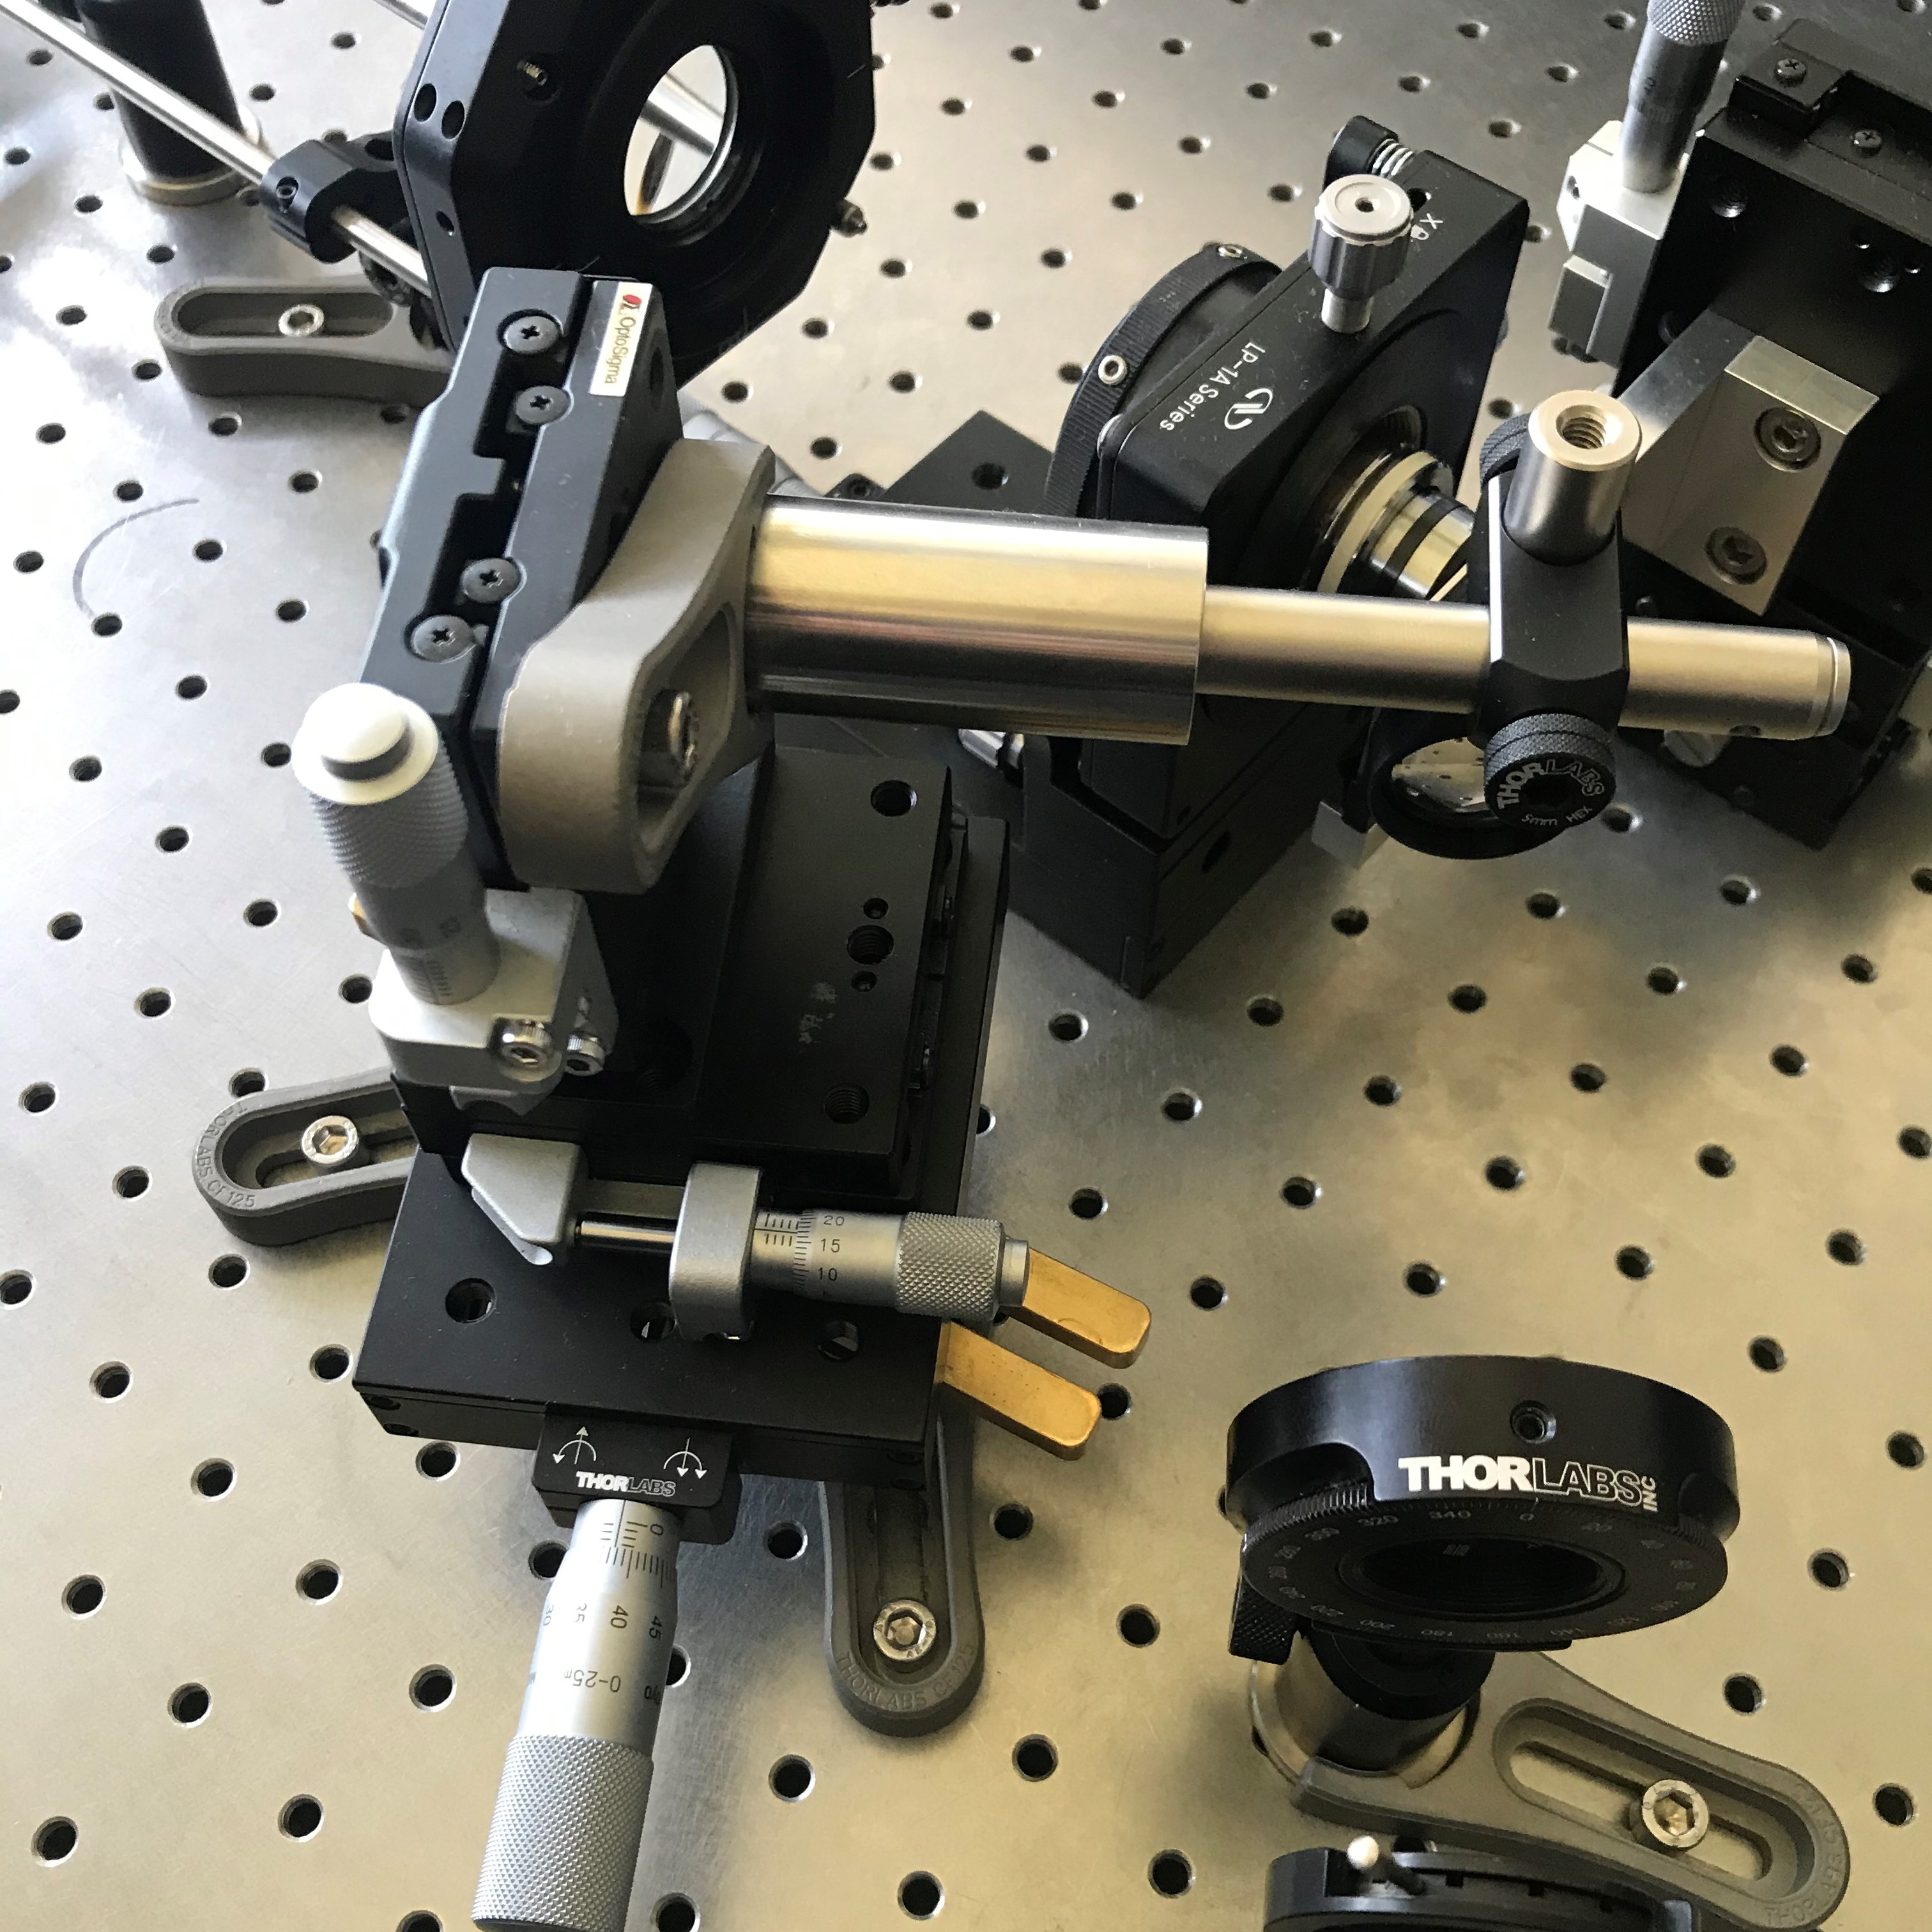
\includegraphics[width=\textwidth]{figures/Einkoppellinse.jpg}
			\caption{Querarm}
			\label{fig:querarm}
		\end{subfigure}
		\hfill
		\begin{subfigure}[b]{0.4\textwidth}
			\centering
			\includegraphics[width=\textwidth]{figures/Kollision_Einkoppellinse.jpg}
			\caption{Kollision Linse mit Probe}
			\label{fig:kollision}
		\end{subfigure}
		\caption[Einkoppellinse-Halterung]{Diese Abbildungen zeigen die Linsenhalterung, welche über einen Querarm an einer xyz-Verfahreinheit montiert ist, und die Kollision zwischen Linsenhalterung und Probe}
		\label{fig:linsenhalterung}
	\end{figure}
	
	\paragraph{Probenhalterung}
	Die Probenhalterung des alten Aufbaus wies das Problem auf, dass die senkrechte Ausrichtung der Probe zur optischen Achse nur grob per Auge erfolgen konnte. Dadurch war beim Verfahren der Probe ein ständiges Nachfokussieren erforderlich. Außerdem fehlte der Halterung die ausreichende Stabilität, was die Fokussierung zusätzlich erschwerte. Daher wurde im Rahmen dieser Arbeit eine neue Probenhalterung entwickelt, konstruiert und die zentrale Werkstatt im Physikzentrum mit der Fertigung beauftragt. Eine technische Zeichnung der Probenhalterung ist im Anhang \ref{fig:tz_probenhalter} zu finden. Diese Probenhalterung behebt die Schwachstellen der alten und hat außerdem einen Anschlag für die Probe, so dass es nun prinzipiell möglich ist, anhand der Skalen an den Mikrometerschrauben der Verfahreinheit Koordinaten abzulesen. So wird ermöglicht, trotz eines Probenwechsel später wieder die gleichen Orte auf der Probe anzufahren.
	\begin{figure}[htbp] 
		\centering
		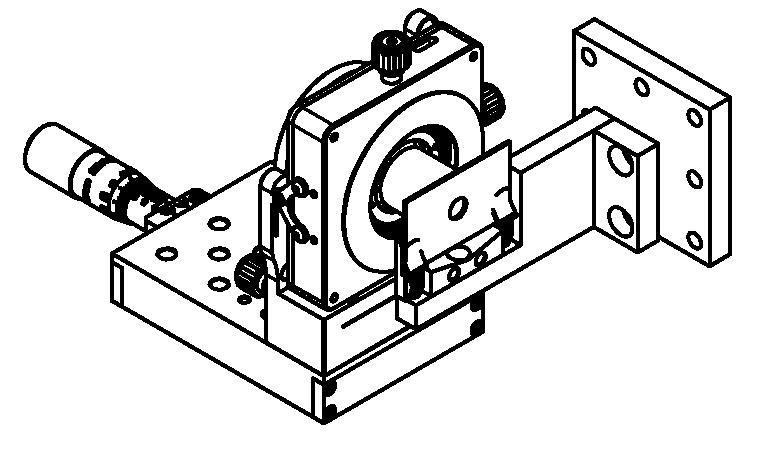
\includegraphics[width=0.5\textwidth]{figures/Probenhalter.pdf}
		\caption[Probenhalterung]{Probenhalter mit montierter Probe vor dem Immersionsobjektiv}
		\label{fig:probenhalter}
	\end{figure}
	\paragraph{Cage-System}
	Sämtliche Optiken hinter dem Immersionsobjektiv wurden in ein Cage-System der Firma \textit{Thorlabs} integriert. Der Umbau auf die Cage-System-Optomechaniken wurde zunächst vollständig in einer CAD-Software geplant (Abbildung \ref{fig:cage_system}). Das Cage-System besteht aus quadratischen Halterungen, die in ihren Eckpunkten Bohrungen haben, durch welche sich Edelstahlstäbe schieben lassen. Diese Fixierung der Halterungen an vier Punkten verhindert ein Verkippen der Linsen entlang der optischen Achse. Die Halterungen können entlang der optischen Achse auf den vier Eckstäben verschoben werden. Für die  Linsen TL, L1, L2 wurden xy-Halter verwendet, die senkrecht zur optischen Achse mit feinen Justierschrauben sehr genau verstellt werden können. Im Laufe dieser Arbeit hat sich herausgestellt, dass diese sehr feine Justierung nicht notwendig gewesen wäre, da der Aufbau äußerst unempfindlich auf kleine Fehler in der Justage der Linsen reagiert. Die Tubuslinse (TL) des Herstellers \textit{Zeiss} ist in einem Halter mit einem $M32\times0.5$ Gewinde montiert. Eine technische Zeichnung der Tubuslinse ist in Abbildung \ref{fig:tubelensetz} zu finden. Für dieses Gewinde stellt \textit{Thorlabs} keine Komponenten her, deswegen war ein Adapter notwendig. Dieser Adapter wurde im Rahmen dieser Arbeit entwickelt und konstruiert und dann von \textit{Sönke Harm} gefertigt. Eine technische Zeichnung dieses Adapters ist in Abbildung \ref{fig:tz_adapter} zu finden. Die optionale Linse (OL) wurde mit einer Magnethalterung in das Cage-System eingebaut. Diese Halterung ermöglicht es, die Linse sehr einfach zu entfernen und so zwischen der Darstellung der Image-Plane und der Backfocal-Plane (BFP) beziehungsweise der Darstellung des Ortsraumes und der Darstellung des Impulsraumes zu wechseln. Außerdem wurde die OL in einem längeren Gewindetubus montiert, so dass ein präzises Verfahren der Linse entlang der optischen Achse möglich ist. Dies ist notwendig, um die BFP exakt zu fokussieren. Ist die richtige Position der OL einmal bestimmt, kann der Gewindetubus mit einem Gewindering gekontert werden. Auch der CMOS-Sensor der Firma \textit{Allied-Vision} wurde in das Cage-System integriert. Hierfür war ein Adapter von der Kameraobjektiv-Gewindenorm \textit{C-Mount} auf die Gewindenorm \textit{SM-2} des Cage-System Herstellers \textit{Thorlabs} notwendig. Eine technische Zeichnung des Cage-System-Aufbaus ist im Anhang in Abbildung \ref{fig:tz_cage_system} zu finden. Der Beam-Block (BB) und der Image-Filter (IF) sind mit Magnetsäulen direkt auf dem optischen Tisch befestigt.
	\begin{figure}[htbp] 
		\centering
		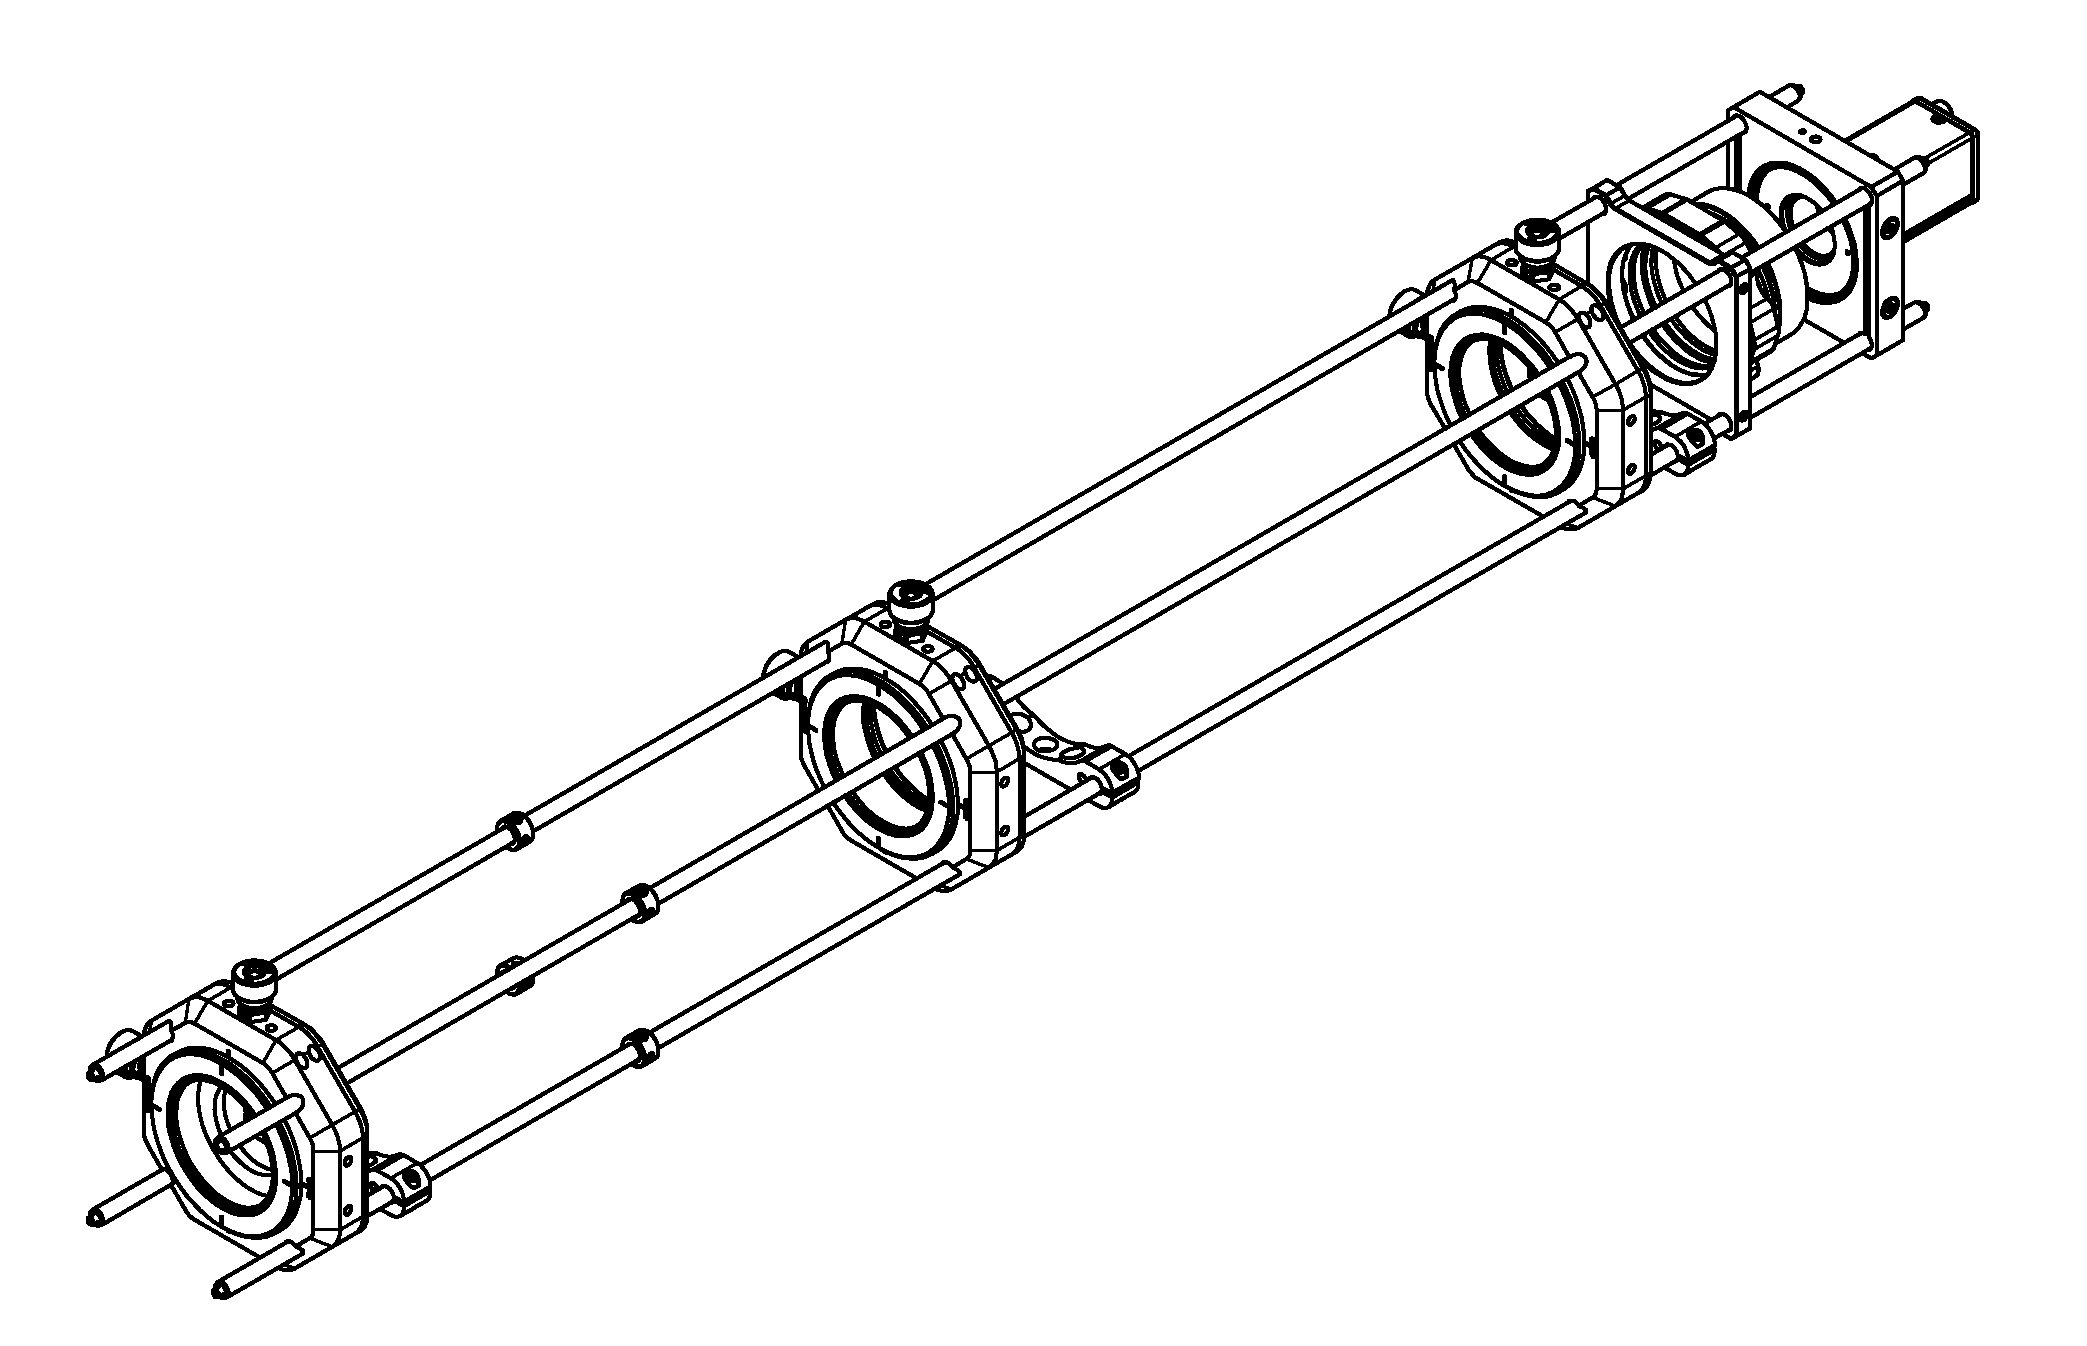
\includegraphics[width=0.7\textwidth]{figures/Cage_System.pdf}
		\caption[Cage-System]{Tubuslinse, 4f-System, optionale Linse und CMOS im Cage-System}
		\label{fig:cage_system}
	\end{figure}	
	\subsection{Probe}
	Die ersten Messungen dieser Arbeit wurden mit Proben, die noch durch die Messungen von \textit{Joris Jaruschewski} \cite{Jaruschewski.2020} vorhanden waren, durchgeführt. Da diese Proben jedoch auch auf der Goldseite mit Immersionsöl kontaminiert waren, wurden später neue Proben verwendet. Diese Proben wurden von \textit{Till Leißner} in S\o nderborg hergestellt. Hierfür wurden Deckgläser der Firma \textit{Carl Zeiss} mit einem Brechungsindex von $n_{\mathrm{Glas}}= 1.52$ verwendet. Die Deckgläser wurden mit einer $d_{\mathrm{Gold}} = 50\mathrm{nm}$ dicken Goldschicht bedampft. Die Deckgläser haben eine Dicke von $d_{\mathrm{Glas}} = 170 \mathrm{\mu m}$. Als Anregungsstruktur wurden Defektstellen verwendet. Die Proben wurden in kleine Edelstahlbleche (Technische Zeichnung \ref{fig:tz_probenblech}) eingeklebt, welche wiederum in die Probenhalterung passen. Damit die Proben auf der Goldseite nicht mit Immersionsöl kontaminiert werden, wurden sie mit einem Epoxid-Kleber in die Edelstahlbleche abdichtend eingeklebt.
	\begin{figure}
		\centering
		\begin{subfigure}[b]{0.4\textwidth}
			\centering
			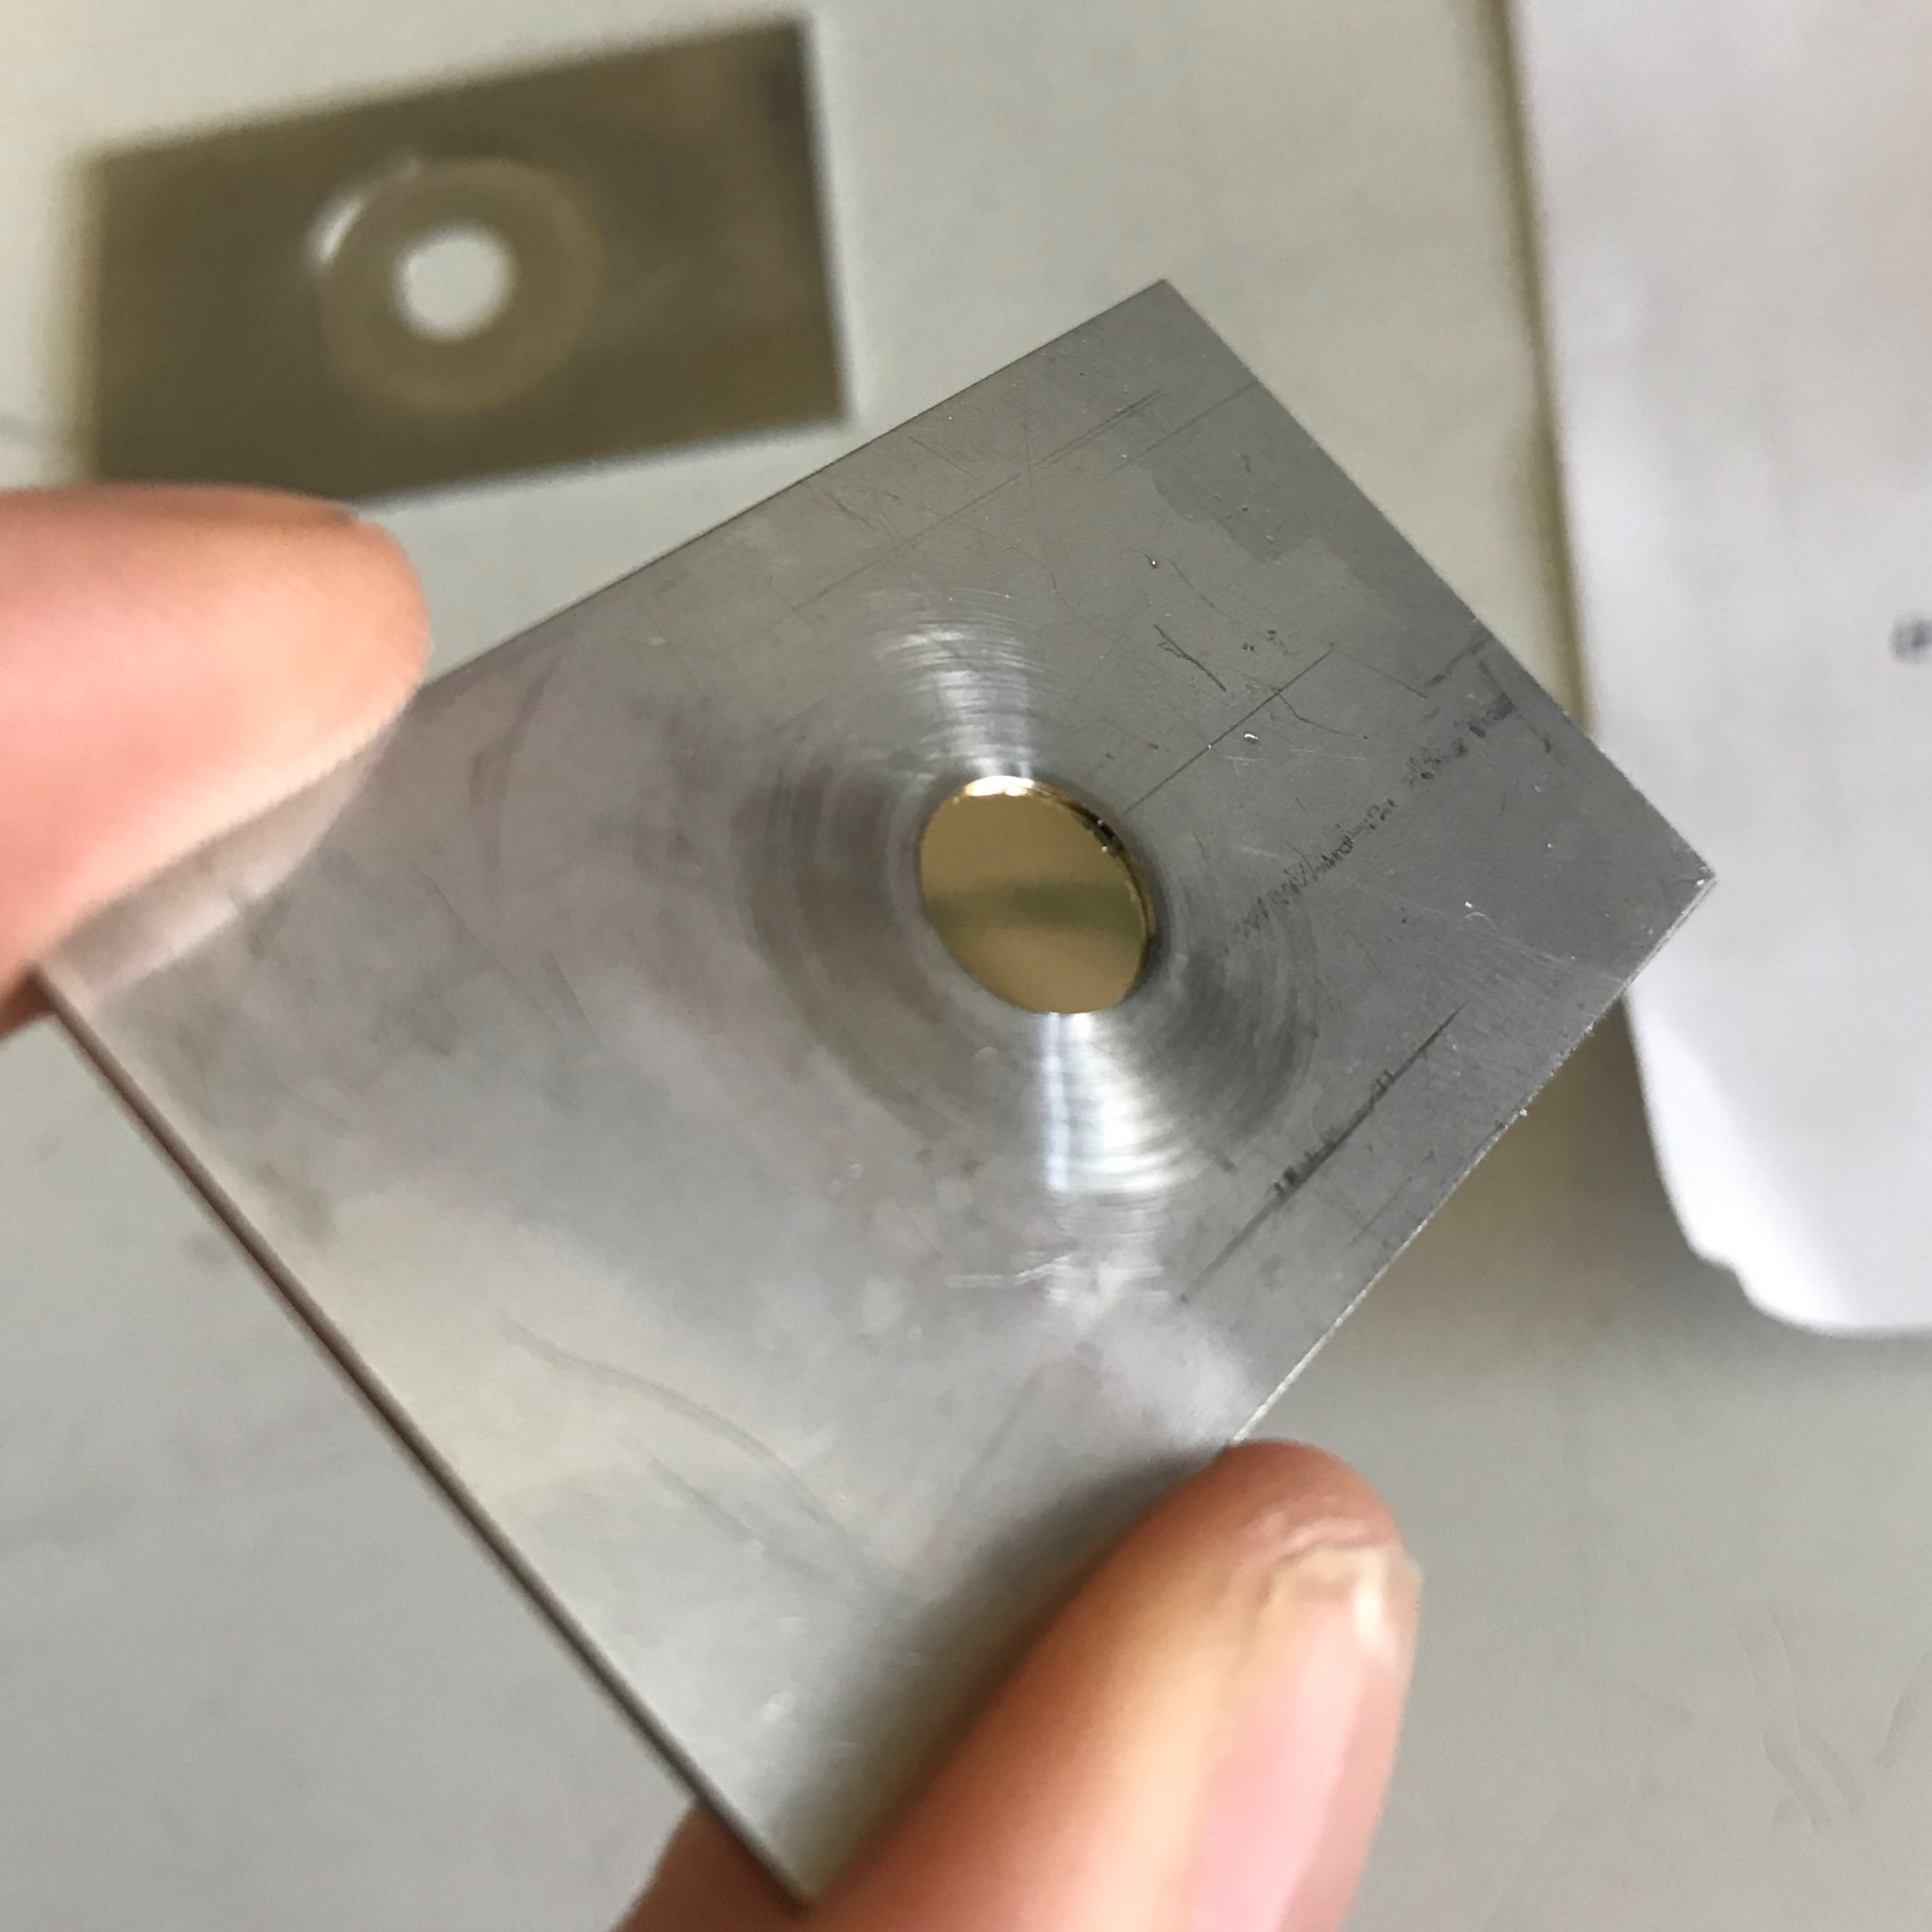
\includegraphics[width=\textwidth]{figures/Probe_Vorderseite.jpg}
			\caption{Goldseite}
			\label{fig:probe_vorderseite}
		\end{subfigure}
		\hfill
		\begin{subfigure}[b]{0.4\textwidth}
			\centering
			\includegraphics[width=\textwidth]{figures/Probe_Rueckseite.jpg}
			\caption{Glasseite}
			\label{fig:probe_rueckseite}
		\end{subfigure}
		\caption[Eingeklebte Probe]{Die Bilder zeigen die in das Edelstahlblech eingeklebte Probe. In rot ist die Verklebung markiert. Hierbei war darauf zu achten, dass die Klebung dicht ist, so dass kein Öl von der Glasseite auf die Goldseite laufen kann.}
		\label{fig:probe}
	\end{figure}
	\subsection{Justage des Aufbaus}
	Die allgemeine Justage des LRM verlief - bis auf die Justage des Lasers auf die Probe - wie von \textit{Joris Jaruschewski} \cite{Jaruschewski.2020} beschrieben. Dieses war durch den notwendigen schrägen Einfall des Lasers auf die Probe deutlich erschwert. Die Justage erfolgte mit montierter Probe. Zunächst wurde die Probe mit Hilfe der Hintergrundbeleuchtung in den korrekten Abstand zum IO gebracht (im korrekten Abstand ist das Bild der Probe scharf zu sehen). Als nächstes wurde der Laser mit zwei Spiegeln grob in dem erwünschten Winkel auf die Probe justiert. Danach wurden Einkoppellinse, $\lambda/4$-Plättchen und Polarisationsfilter in den Strahlgang gestellt. Die Feinjustierung des Lasers auf die Probe wurde nun durch das Verschieben der Einkoppellinse durchgeführt. Hierbei ist es hilfreich, den Strahl durch das Verfahren der EL entlang der optischen Achse etwas zu de-fokussieren, so dass man die Randbereiche des Strahls über den CMOS-Sensor in der Image-Plane auch schon sehen kann, wenn der Strahl noch nicht exakt die optische Achse trifft. Sobald ein Teil des Strahls in der Image-Plane detektiert worden ist, wird er durch weiteres Bewegen der Linse zentriert und dann schrittweise weiter fokussiert. Durch das Verkippen der Einkoppellinse zum Laser wandert der Strahl beim Fokussieren des Lasers auf der Probe aus. Das Verkippen der Linse wird behoben, sobald der Laser optimal fokussiert ist. Hierfür wird der Laser durch die beiden Spiegel sukzessive so einjustiert, dass der Spot auf der Probe beim Defokussieren des Lasers nicht mehr wandert.
	
		
	\subsection{Messung}
	Zunächst wurde die Funktionsfähigkeit des LRM durch einige Probemessungen überprüft, die mit den Daten von \textit{Jaruschewski} \cite{Jaruschewski.2020} und \textit{Ebel} \cite{ebel.2019} verglichen worden sind. Da für den Nachweis des PSHE keine Kenntnis des Betrages des Wellenvektors notwendig ist, wurde auf eine Kalibrierung der BFP verzichtet. Die in den Abbildungen dargestellten Skalen von $|\vec{k}_{\mathrm{SPP}}|$ und $|\vec{r}|$ wurden aus der Kalibrierung von \textit{Jaruschewski} errechnet. Die Polarisation des Lasers wurde so ausgerichtet, dass sie bei Orientierung des $\lambda/4$-Plättchen $\alpha_{\lambda/4} \in \{0^\circ, 90^\circ, 180^\circ, 270^\circ\}$ parallel zur Einfallsebene des Lasers liegt.  Dann wurde ein geeigneter Defekt auf der Probenoberfläche ausgewählt. Das Vorgehen hierbei bestand darin, die Probe zu verfahren und dabei die Anregung im Impulsraum zu beobachten. Sobald der Laser hierbei auf einen Defekt trifft, ist in der Impulsdarstellung die charakteristische Leckstrahlung zu erkennen. Das Ziel war, einen Defekt zu finden, der möglichst symmetrisch abstrahlt. Nachdem ein geeigneter Defekt ausgewählt war, wurden Bilder des Ortsraumes und des Impulsraumes für unterschiedliche Orientierungen des $\lambda/4$-Plättchen bei gleichbleibender Belichtungszeit aufgenommen.
	\subsection{Verarbeitung der Messdaten}
	\label{sec:polar_calculation}
	Die Messdaten wurden in der Programmiersprache Python mit den Bibliotheken \textit{Numpy}, \textit{OpenCV}, \textit{Scipy} und \textit{Matplotlib} verarbeitet. Die mit dem CMOS-Sensor aufgenommen Bilder wurden im Windows Bitmap Format (BMP) mit einer Bittiefe von  $b = 8$ gespeichert. Die Auflösung der verwendeten Sensors beträgt $2592 \times 1944$. Der verwendete CMOS-Sensor liefert auch eine Farbinformation. Jeder Bildpunkt der BMP-Datei besteht aus einem Rot, einem Grün und einem Blau Wert zwischen $0$ und $2^b - 1= 255$. Ein CMOS Sensor ist nicht Wellenlängen sensitiv. Die Farbinformation wird durch eine Filtermatrix vor dem CMOS Sensor gewonnen. Die unterschiedlichen Farbdaten könnten genutzt werden, um Informationen über das Spektrum der detektierten Strahlung zu erlangen, dass war in dieser Arbeit allerdings nicht von Interesse, da die Leckstrahlung monochromatisch ist (mit der gleichen Wellenlänge, wie die anregende Strahlung). Deswegen wurde aus den RGB-Werten das arithmetische Mittel berechnet. Die Intensität wurde so skaliert, dass der maximale Werte 1 entspricht. Die Aufnahme des Orts und des Impulsraumes wurden zunächst von den kartesischen Pixel-Koordinaten in Polarkoordinaten transformiert, da dies die weitere Auswertung stark vereinfacht. Als Ursprung wurde dabei im Impulsraum der Mittelpunkt der Kreisförmigen Begrenzung der Impulsdarstellung durch die numerische Apertur, und im Ortsraum das Anregungszentrum gewählt. Um aus den äquidistanten Pixel-Koordinaten ein äquidistantes Gitter in Polarkoordinaten zu erzeugen, mussten die Daten interpoliert werden. Diese Interpolation wurde mit der Funktion \textit{linearPolar()} im Modus \textit{INTER\_CUBIC} aus der Bibliothek \textit{openCV} ausgeführt. Die so gewonnenen Daten in Polarkoordinaten konnten nun mit Hilfe der \textit{matplotlib} dargestellt werden. Für die weitere Auswertung musste unter anderem ein radiales Profil berechnet werden, in Polarkoordinaten wird diese Integration zu einer einfachen Summe über eine Achse. Für die Analyse des Spin-Hall Effektes mussten Intensitäten in bestimmten Masken integriert werden. Auch diese Integration hat sich durch die Verwendung von Polarkoordinaten stark vereinfacht. Der gesamte in dieser Arbeit geschriebene Quellcode wird unter \url{https://github.com/hanno22/SpinHallEffectThesis} zur Verfügung gestellt.
	\newpage
	
	\section{Ergebnisse und Diskussion}
	
	\subsection{Überprüfung der Funktionsfähigkeit des LRM}
	In diesem Abschnitt soll verifiziert werden, dass die Messdaten des LRM tatsächlich plasmonischer Natur sind.
	\subsubsection{Verunreinigte Proben}
	Die ersten Testmessungen wurden an Proben durchgeführt, die noch aus vorangegangenen Arbeiten vorhanden waren. Diese Proben waren sowohl auf der Goldseite als auch auf der Glasseite mit Immersionsöl kontaminiert. Diese Kontamination sorgte dafür, dass die Anregung im $k$-Raum ein deutlich breiteres Spektrum aufweist als die später durchgeführten Messungen an nicht kontaminierten Proben (diese Messung wird im Anhang \ref{fig:dirt_polar} dargestellt). Dies ist durch Dämpfungseffekte durch das Öl auf der Probe zu erklären. Eine der Proben wurde mit Ethanol gereinigt und anschließend die Messung wiederholt. Die Kontamination konnte so weitestgehend entfernt werden, und die Anregung zeigt ein deutlich schmaleres Spektrum. Allerdings wurde die Probe durch die Reinigung mechanisch so stark beschädigt, dass die Defektdichte zu hoch war, um einen Defekt mit einer Umgebung ohne Fehlstellen zu finden. Insbesondere hat die Reinigung zu Kratzern auf der Goldoberfläche geführt, die scharfe Beugungskanten in der Impulsdarstellung  erzeugen. Für den weiteren Verlauf der Arbeit wurden daher neue Proben hergestellt. Diese Proben wurden statt mit Leitsilber mit Epoxidkleber abdichtend in die Probenbleche eingeklebt, so dass keine erneute Kontamination mit Immersionsöl auftreten konnte.
	\subsubsection{Bestimmung von  $k_{\mathrm{spp}}$ an neuer Probe}
	Zur Bestimmung von $k_{\mathrm{spp}}$ wurde die Anregung an einem Punktdefekt bei einem Einfallswinkel $\alpha_{\mathrm{E}} = 60^\circ$ bei linearer Polarisation parallel zur Einfallsebene untersucht. Da die Begrenzung der BFP durch die NA nur vom Immersionsobjektiv und dem Brechungsindex des verwendeten Immersionsöls abhängt, ist diese Begrenzung gut geeignet, um eine Kalibrierung der BFP durchzuführen. In der vorliegenden Arbeit wird sowohl das gleiche Immersionsöl als auch das gleiche Immersionsobjektiv wie in der Arbeit \cite{Jaruschewski.2020} verwendet, daher kann die Kalibrierung aus dieser Arbeit übernommen werden. Dort wurde durch eine SPP-Mode mit bekanntem $k_{\mathrm{spp}}$ der Wert der numerischen Apertur der Kombination Immersionsobjektiv-Immersionsöl bei einer Wellenlänge von $\lambda=633\mathrm{nm}$ auf $\mathrm{NA}_{\lambda = 633 \,\mathrm{nm}} = 1.216 \pm 0.005$  und $k_0\mathrm{NA}_{\lambda = 633 \, \mathrm{nm}} = 12.07 \pm 0.05\,\mathrm{\mu m}^{-1}$ bestimmt. Anhand dieser Kalibrierung wurde der Wert von $k_{\mathrm{spp}}$ bestimmt. Hierfür wurde das Integral:
	\begin{equation}
		P_k\left(|\vec{k}_{\bot}|\right) := \int_{0}^{2 \pi} I_k\left(|\vec{k}_{\bot}|, \phi\right)\mathrm{d}\phi
	\end{equation}	 
	ausgewertet. Hierbei ist $I_k\left(|\vec{k}_{\bot}|, \phi\right)$ die Intensitätsverteilung in der Impulsdarstellung. Das Maximum dieser radialen Intensitätsverteilung entspricht nach Gleichung \eqref{eq:ext_phase_condition} $k_{\mathrm{spp}}$ und liegt bei $k_{\mathrm{spp}}= 10.35\,\mathrm{\mu m}^{-1}$. Dieser Wert stimmt bis auf $0.2\%$ mit dem Wert aus der theoretischen Berechnung \eqref{eq:theo_k_spp} überein. Allerdings ist hier zu bemerken, dass die Luft-Gold-Glas-Mode auch in \cite{Jaruschewski.2020} für die Kalibrierung genutzt worden ist. Die Messdaten sind in Abbildung \ref{fig:example_bfp} und die radiale Intensitätsverteilung ist in Abbildung \ref{fig:radial_profile} dargestellt. Die Einfallsrichtung des Lasers war hierbei entlang der $0^\circ$-Linie. Es fällt auf, dass die Anregung in Richtung der Einfallsebene deutlich stärker ausgeprägt ist. 
	\begin{figure}
		\label{fig:example_measure}
		\centering
			\begin{subfigure}[b]{0.5\textwidth}
			\centering
			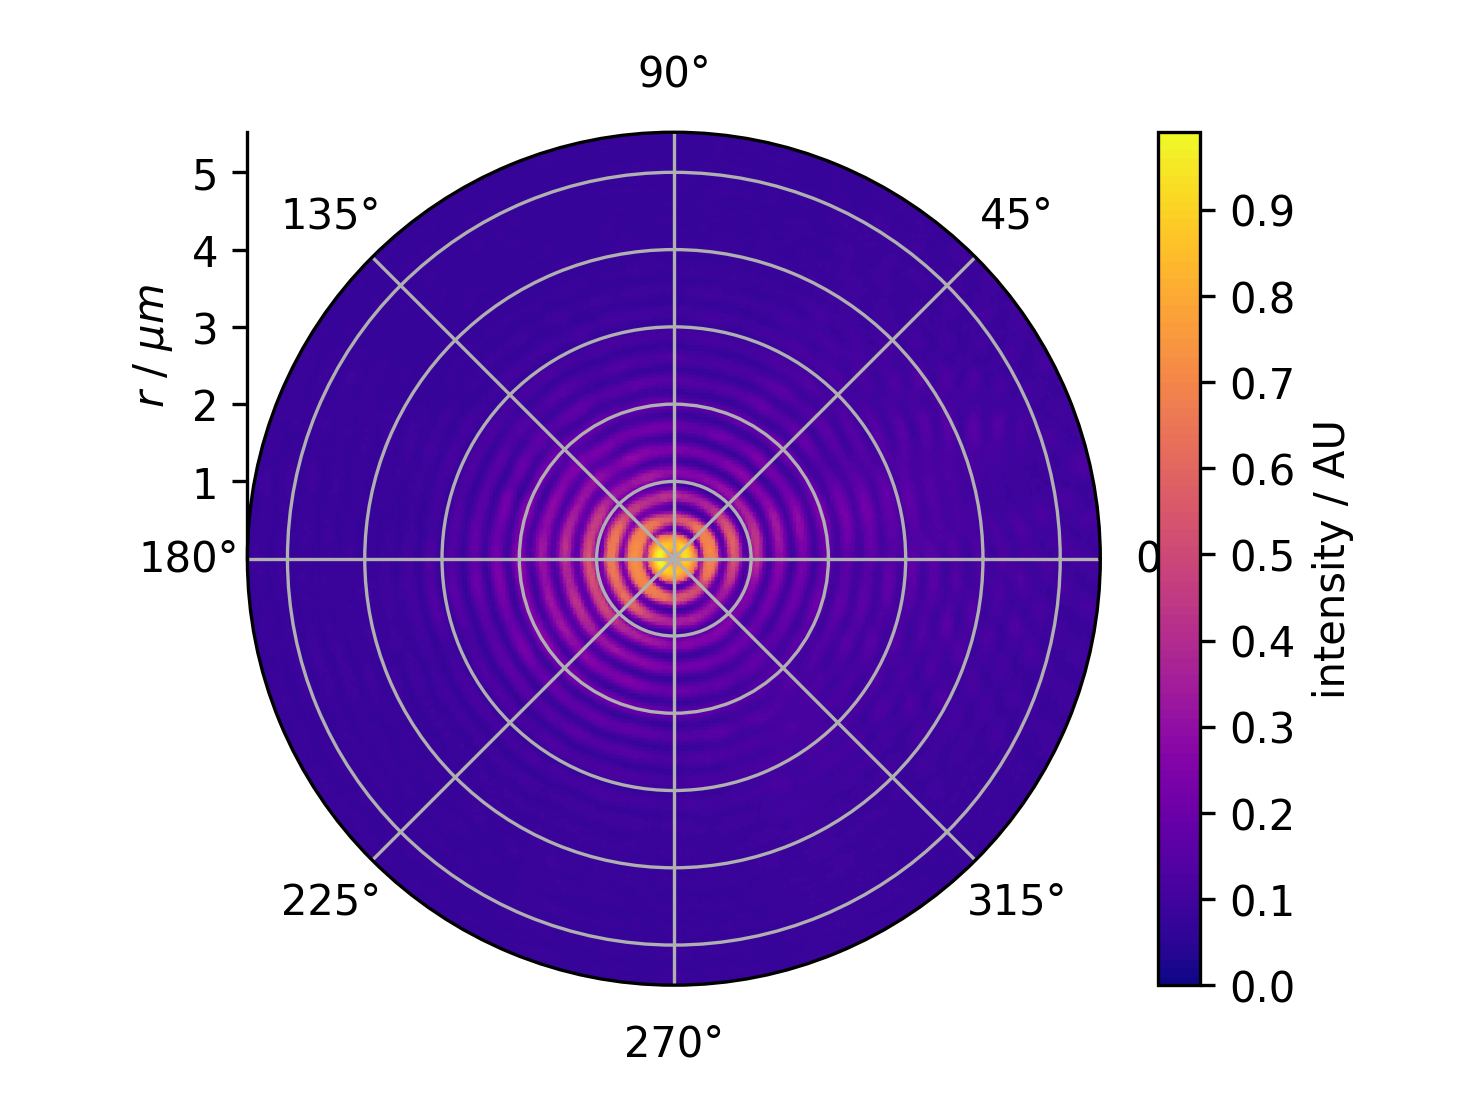
\includegraphics[width=\textwidth]{figures/fp/fp_0.png}
			\caption{Intensitätsverteilung in der FP}
			\label{fig:example_fp}		
			\end{subfigure}
			\begin{subfigure}[b]{0.49\textwidth}
				\centering
				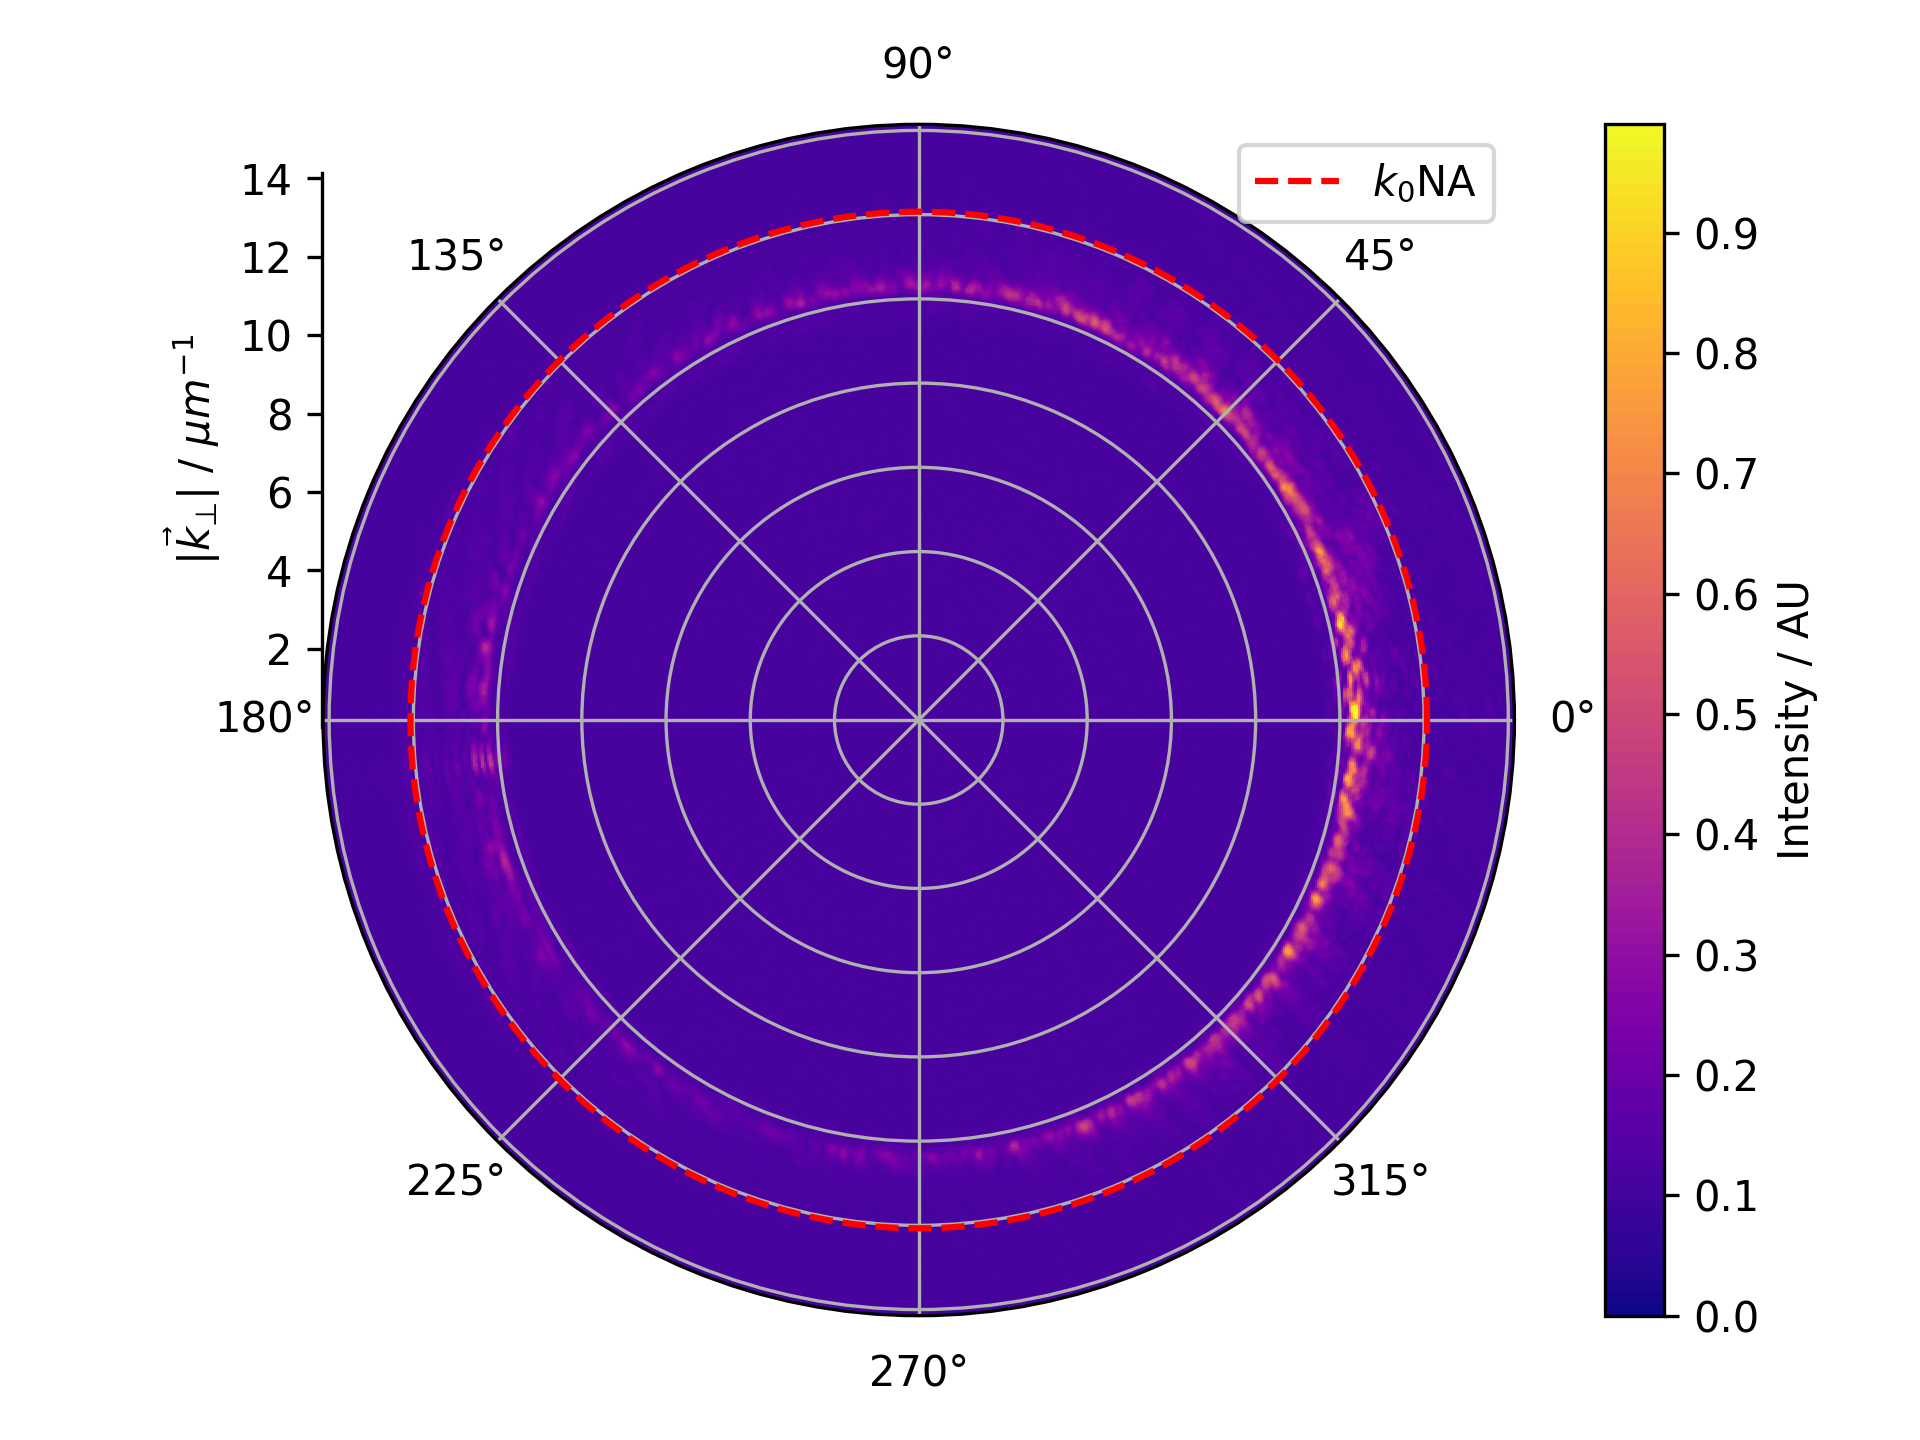
\includegraphics[width=\textwidth]{figures/example_polar.png}
				\caption{Intensitätsverteilung in der BFP}
				\label{fig:example_bfp}		
			\end{subfigure}
			\begin{subfigure}[b]{0.5\textwidth}
					\centering
				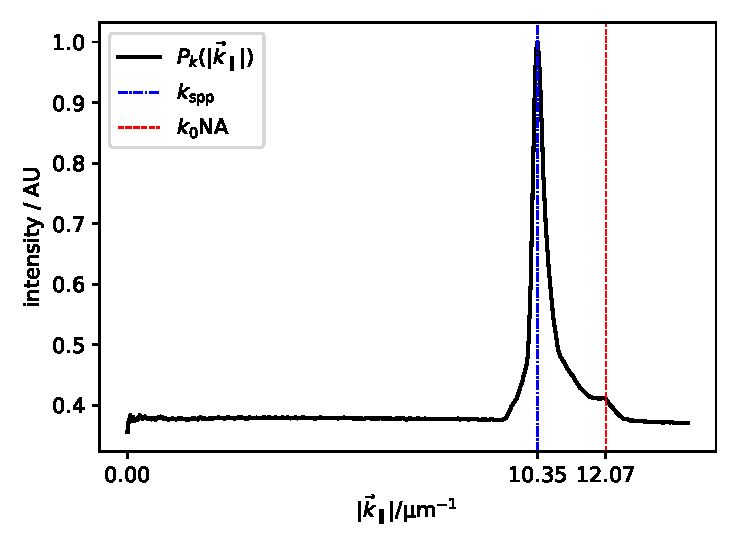
\includegraphics[width=\textwidth]{figures/example_radial.pdf}
				\caption{Radiale Intensitätsverteilung}
				\label{fig:radial_profile}			
			\end{subfigure}
			\hfill
			\begin{subfigure}[b]{0.49\textwidth}
				\centering
				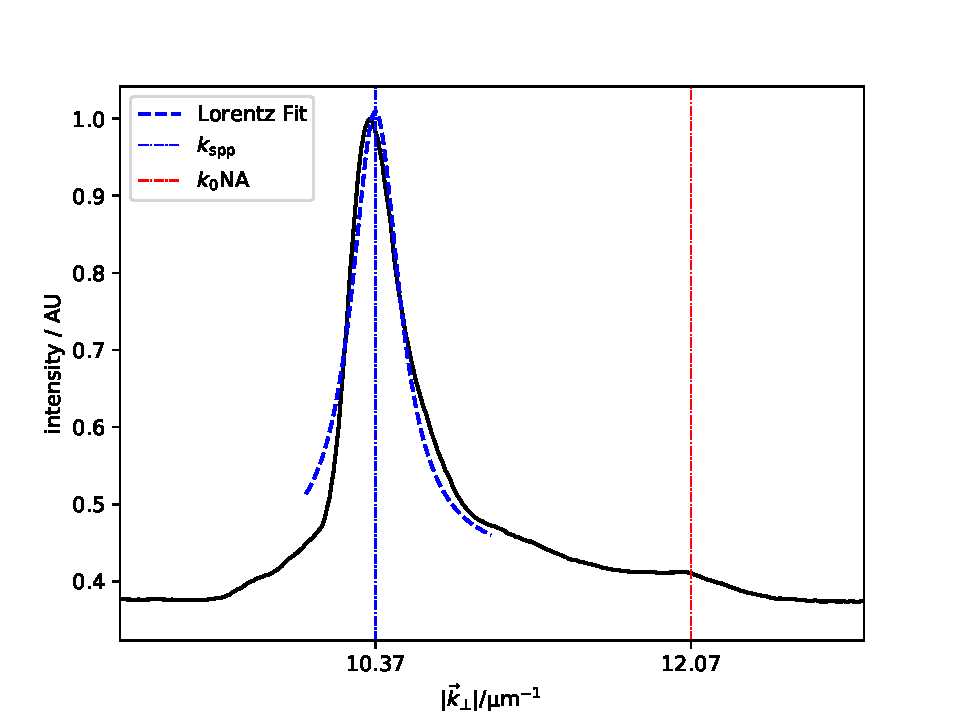
\includegraphics[width=\textwidth]{figures/lorenz_profile}
				\caption{Lorentz-Fit}
				\label{fig:lorenz_profile}			
			\end{subfigure}
	
		\caption[Messwerte bei linearer Polarisation]{Messung unter $\alpha_{\mathrm{E}} = 60^\circ$ bei p-Polarisation.
			Der rot markierte Knick in der Intensitätsverteilung entsteht durch die Begrenzung der BFP durch die NA und wurde ausgenutzt, um die Skala zu kalibrieren. Die radiale Intensitätsverteilung hat ein Maximum bei $k_{\mathrm{spp}}= 10.35\,\mathrm{\mu m ^{-1}}$.}			
	\end{figure}
	Aus der radialen Intensitätsverteilung der BFP lässt sich außerdem der Imaginärteil des Wellenvektors bestimmen. Hierfür  wird ausgenutzt, dass die radiale Intensitätsverteilung der BFP nach \eqref{eq:ext_phase_condition} ein Lorentz-Profil sein sollte. Die Profilbreite wird hierbei durch den Imaginärteil des Wellenvektors bestimmt. Aus den Messdaten lässt sich diese Profilbreite nun über eine Anpassung eines Lorentzprofils mit der Methode der kleinsten Quadrate bestimmen. Diese Fit-Kurve ist in Abbildung \ref{fig:lorenz_profile} dargestellt. Dieser Fit hat $\Im\{k_\mathrm{SPP}\} = 0.16\,\mathrm{\mu m}^{-1}$ ergeben. Die Abweichung von $250\%$ zu dem theoretisch errechneten Wert \ref{eq:theo_k_spp} lässt sich durch zwei Effekte erklären: Erstens kommt es durch Abbildungsfehler in dem LRM zu einer Verbreiterung des Profils in der BFP \cite{Jaruschewski.2020}, daher ergibt die gemessene Profilbreite nur eine obere Schranke für die tatsächliche Dämpfung des SPP. Zweitens ist die genaue Qualität der Probe unbekannt, und weitere Defekte und größere Oberflächenrauigkeiten können zu einer stärkeren Dämpfung des SPP führen. In der Arbeit \cite{Jaruschewski.2020} wurde  $\Im\{k_\mathrm{SPP}\} = 0.19\,\mathrm{\mu m}^{-1}$ gemessen. Dieser Wert weicht um $19\%$ von dem in der vorliegenden Arbeit gemessenen Wert ab. Da die Profilbreite im Vergleich zu \cite{Jaruschewski.2020} kleiner geworden ist, ist davon auszugehen, dass entweder die Probenqualität zugenommen hat oder die Qualität der optischen Abbildung verbessert werden konnte (in \cite{Jaruschewski.2020} wurde das Intensitätsprofil nur entlang einer Linie und nicht über den gesamten Vollkreis berechnet). Hierbei ist anzumerken, dass der Lorentz-Fit äußerst empfindlich auf die Wahl des Fit-Bereichs reagiert. Außerdem ist wie in Abbildung \ref{fig:lorenz_profile} dargestellt der Fit nur eine grobe Näherung und stimmt nicht besonders gut mit den Messdaten überein.	
	
	\subsection{Nachweis des PSHE}
	Zum Nachweis des PSHE wurde mit Hilfe des Leckstrahlmikroskopes die Anregung eines SPPs an einem Punktdefekt in Abhängigkeit der Polarisation der Anregungsstrahlung untersucht. Es wurde für unterschiedliche Orientierungen des $\lambda /4$-Plättchens jeweils eine Intensitätsmessung der Leckstrahlung im Ortsraum und im Impulsraum durchgeführt. Die gemessene Intensitätsverteilung im Ortsraum sei durch $I_r(|\vec{r}|, \phi, \alpha_{\lambda /4})$ und die gemessene Intensitätsverteilung im Impulsraum durch $I_k(|\vec{k}_\perp|, \phi, \alpha_{\lambda /4})$ beschrieben (die Umrechnung der kartesischen Pixeldaten in Polarkoordinaten wird in Abschnitt \ref{sec:polar_calculation} näher erläutert). Hierbei ist $|\vec{r}|$ der radiale Abstand zum Anregungszentrum, $|\vec{k}_\perp|$ der Betrag des Wellenvektor senkrecht zu optischen Achse und $\alpha_{\lambda/4}$ die Orientierung des $\lambda/4$-Plättchens. Der Polarwinkel $\phi$ beschreibt in der Ortsraumdarstellung den Winkel zu einem Ort und in der Impulsdarstellung eine Richtung des Wellenvektors. Da das Koordinatensystem des Ortsraumes so gewählt worden ist, dass das Anregungszentrum im Ursprung liegt, entspricht der Winkel zu einem Punkt im Ortsraum auch gerade dem Winkel des Wellenvektors, der diesen Punkt im Ortsraum erreichen kann. $\phi = 0$ liegt hierbei in der Einfallsebene in Richtung der anregenden Strahlung. Der Impulsraum wurde für unterschiedliche Orientierungen des $\lambda/4$-Plättchens  $\alpha_{\lambda/4} \in [0^\circ,360^\circ)$ mit einer Schrittweite von $2^\circ$ aufgenommen. Das Ortsbild der Anregung wurde mit einer Schrittweite von $20^\circ$ aufgezeichnet.
	
	\subsubsection{Rohdaten}
	Zunächst wurden die Rohdaten bei links- und rechts-zirkular polarisierter Anregungsstrahlung untersucht, also $I_r(|\vec{r}|, \phi, \alpha_{\lambda /4})$ und $I_k(|\vec{k}_\perp|, \phi, \alpha_{\lambda /4})$ für $\alpha_{\lambda /4} \in \{45^\circ, 135^\circ\}$. Diese Daten sind in Abbildung \ref{fig:measure_pshe_raw} dargestellt. 
	\begin{figure}
		\begin{subfigure}[b]{0.49\textwidth}
			\centering
			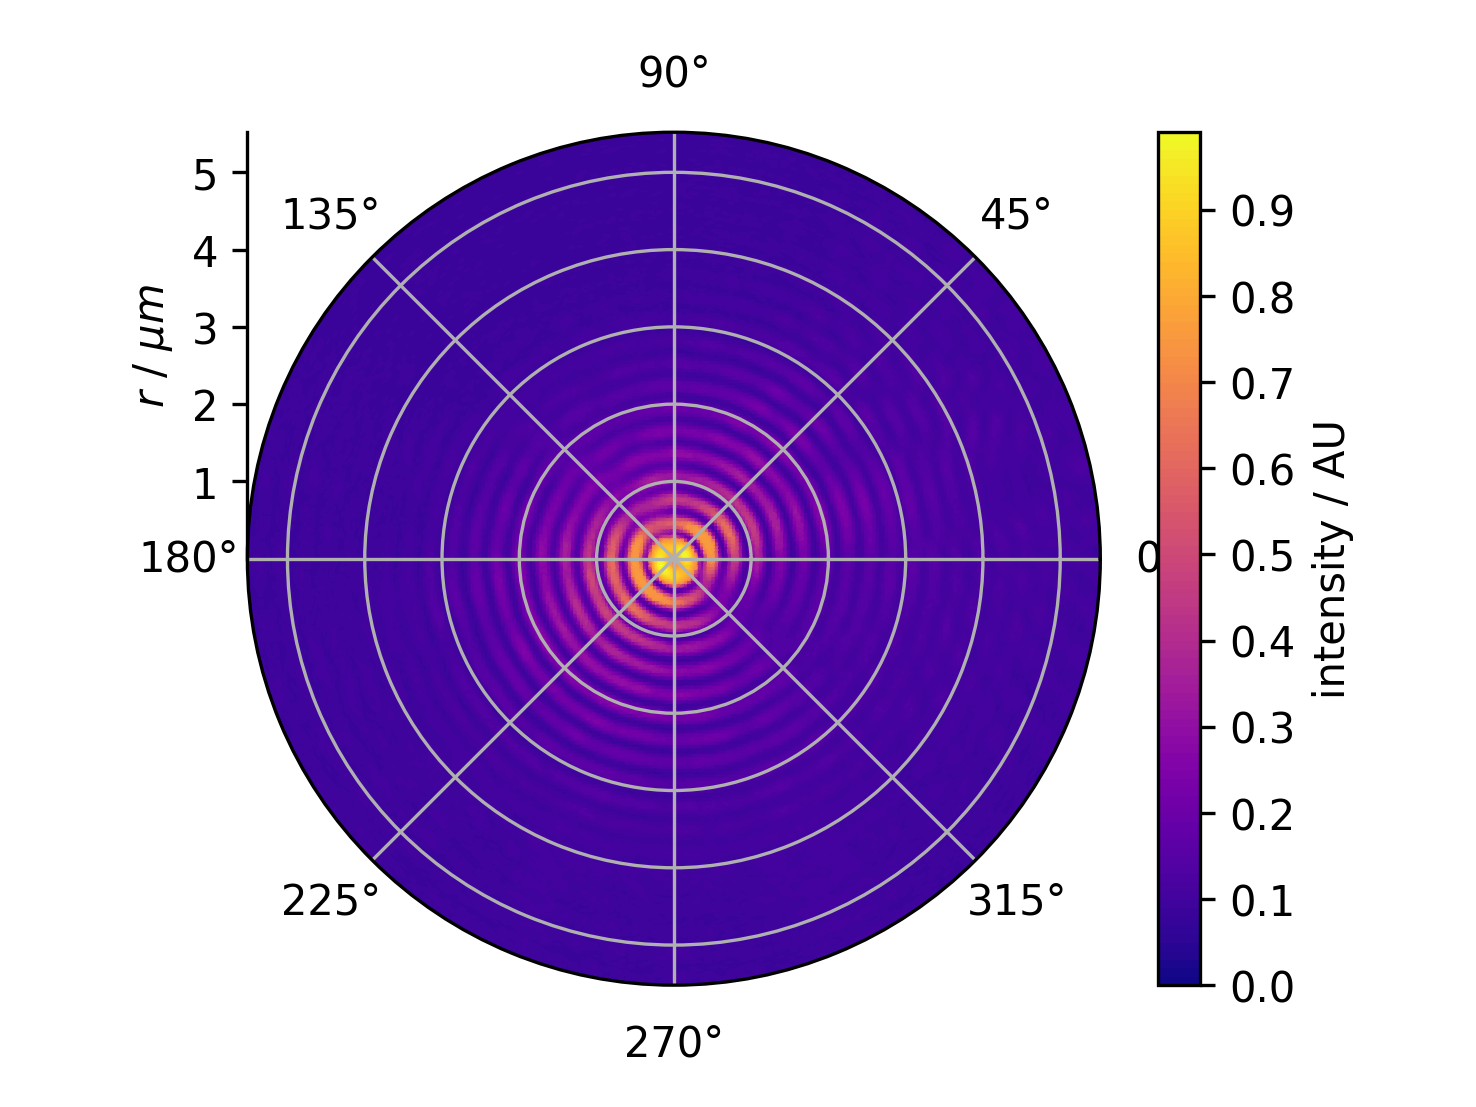
\includegraphics[width=\textwidth]{figures/fp/fp_45.png}
			\caption{$I_r(|\vec{r}|, \phi, \alpha_{\lambda /4} = 45^\circ)$}
			\label{fig:raw_fp_45}
		\end{subfigure}
		\begin{subfigure}[b]{0.5\textwidth}
			\centering
			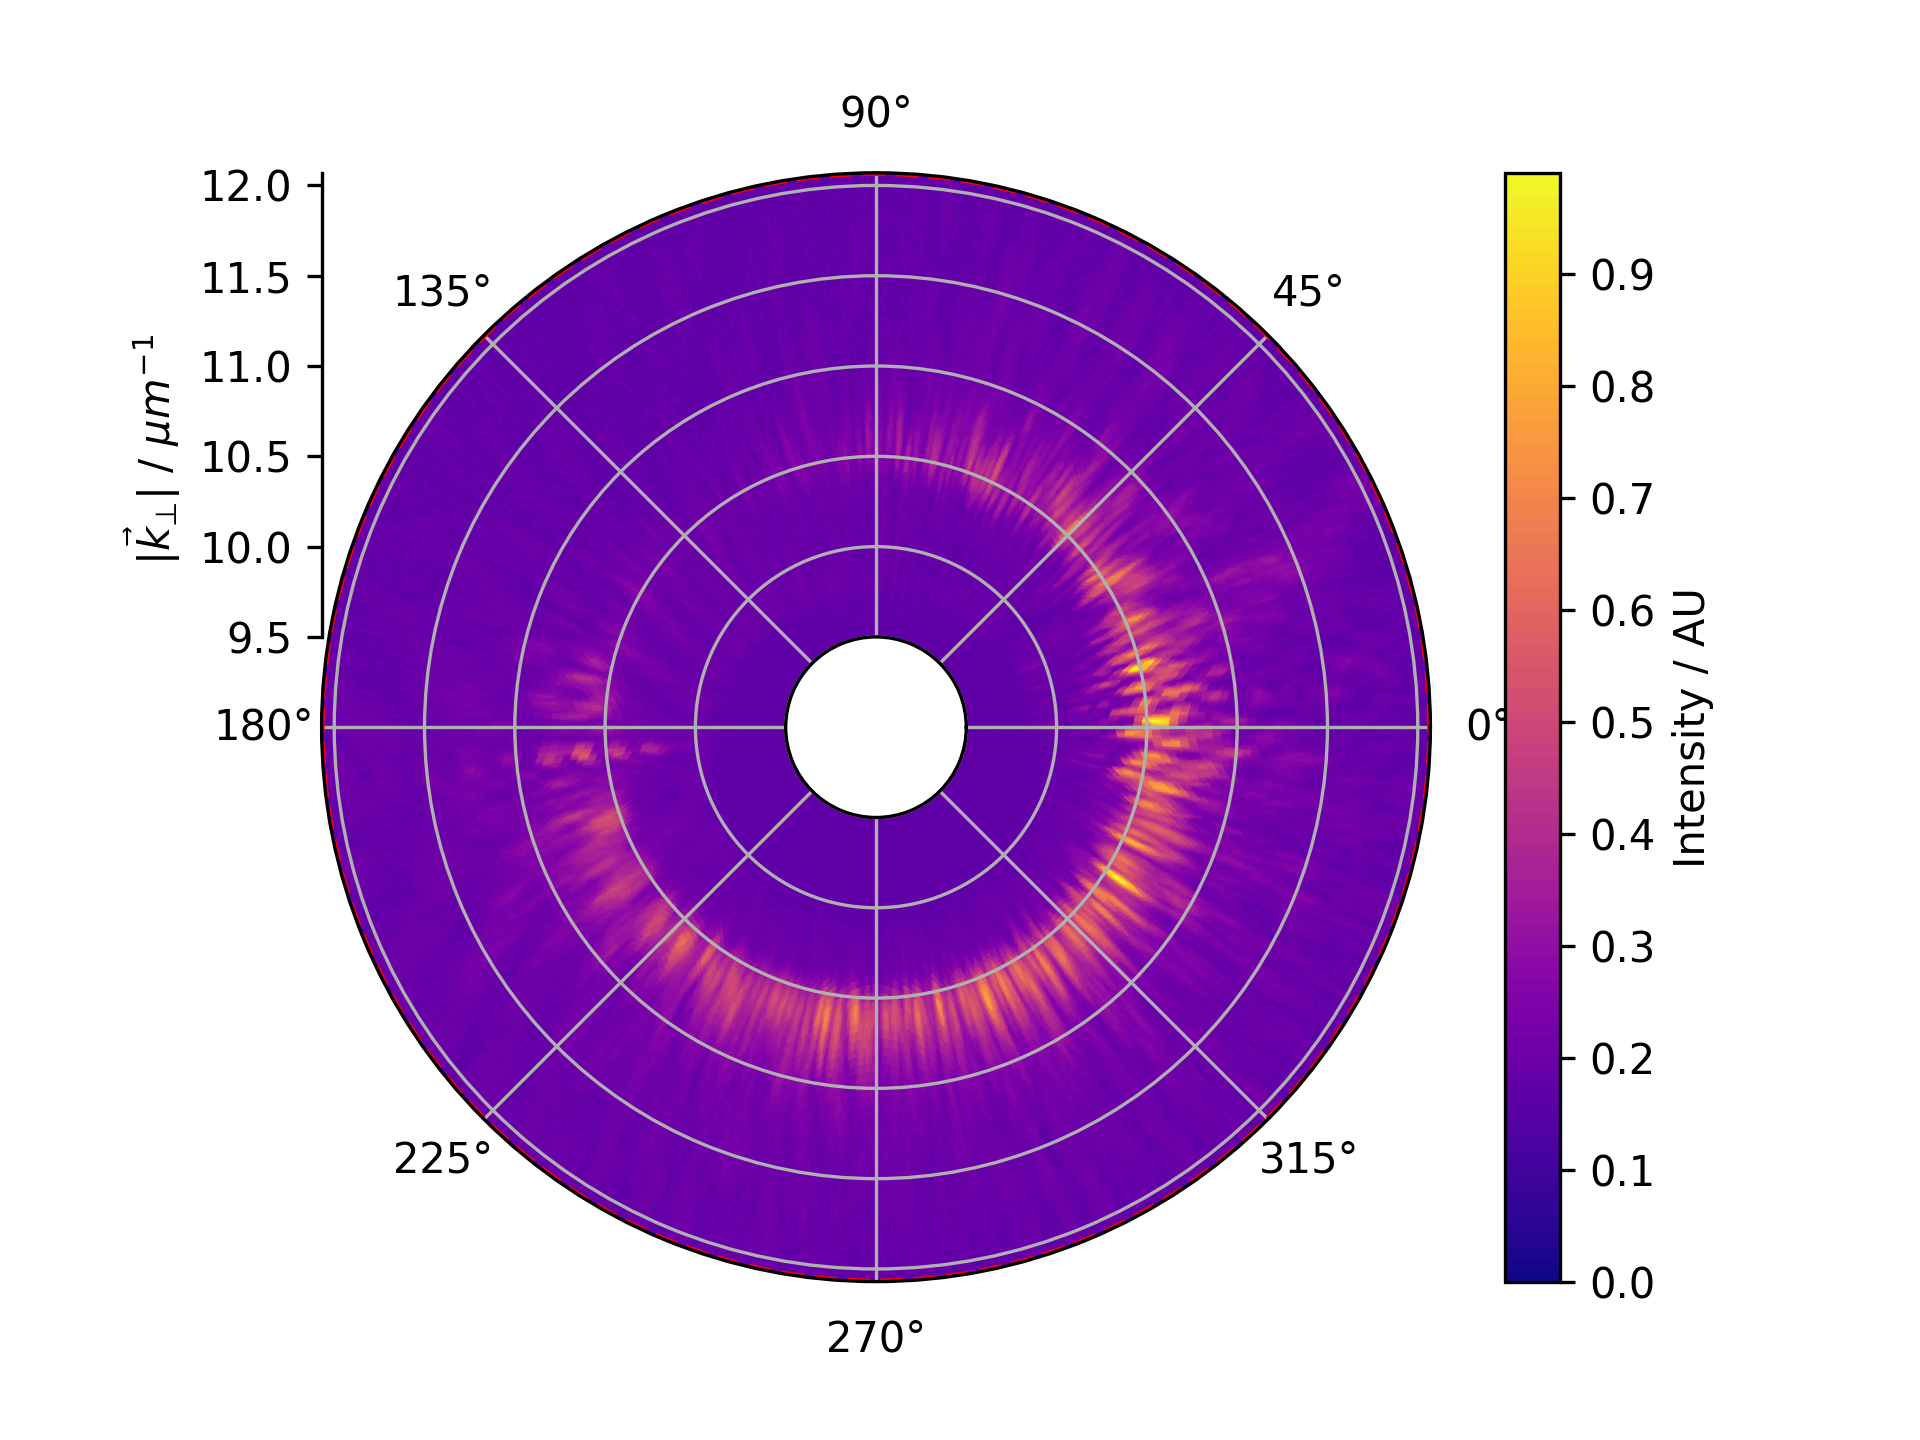
\includegraphics[width=\textwidth]{figures/spin_hall/polar/polar_45.png}
			\caption{$I_k(|\vec{k}_\perp|, \phi, \alpha_{\lambda /4}= 45^\circ)$}
			\label{fig:raw_bfp_45}
		\end{subfigure}		
		\hfill		
		\begin{subfigure}[b]{0.49\textwidth}
			\centering
			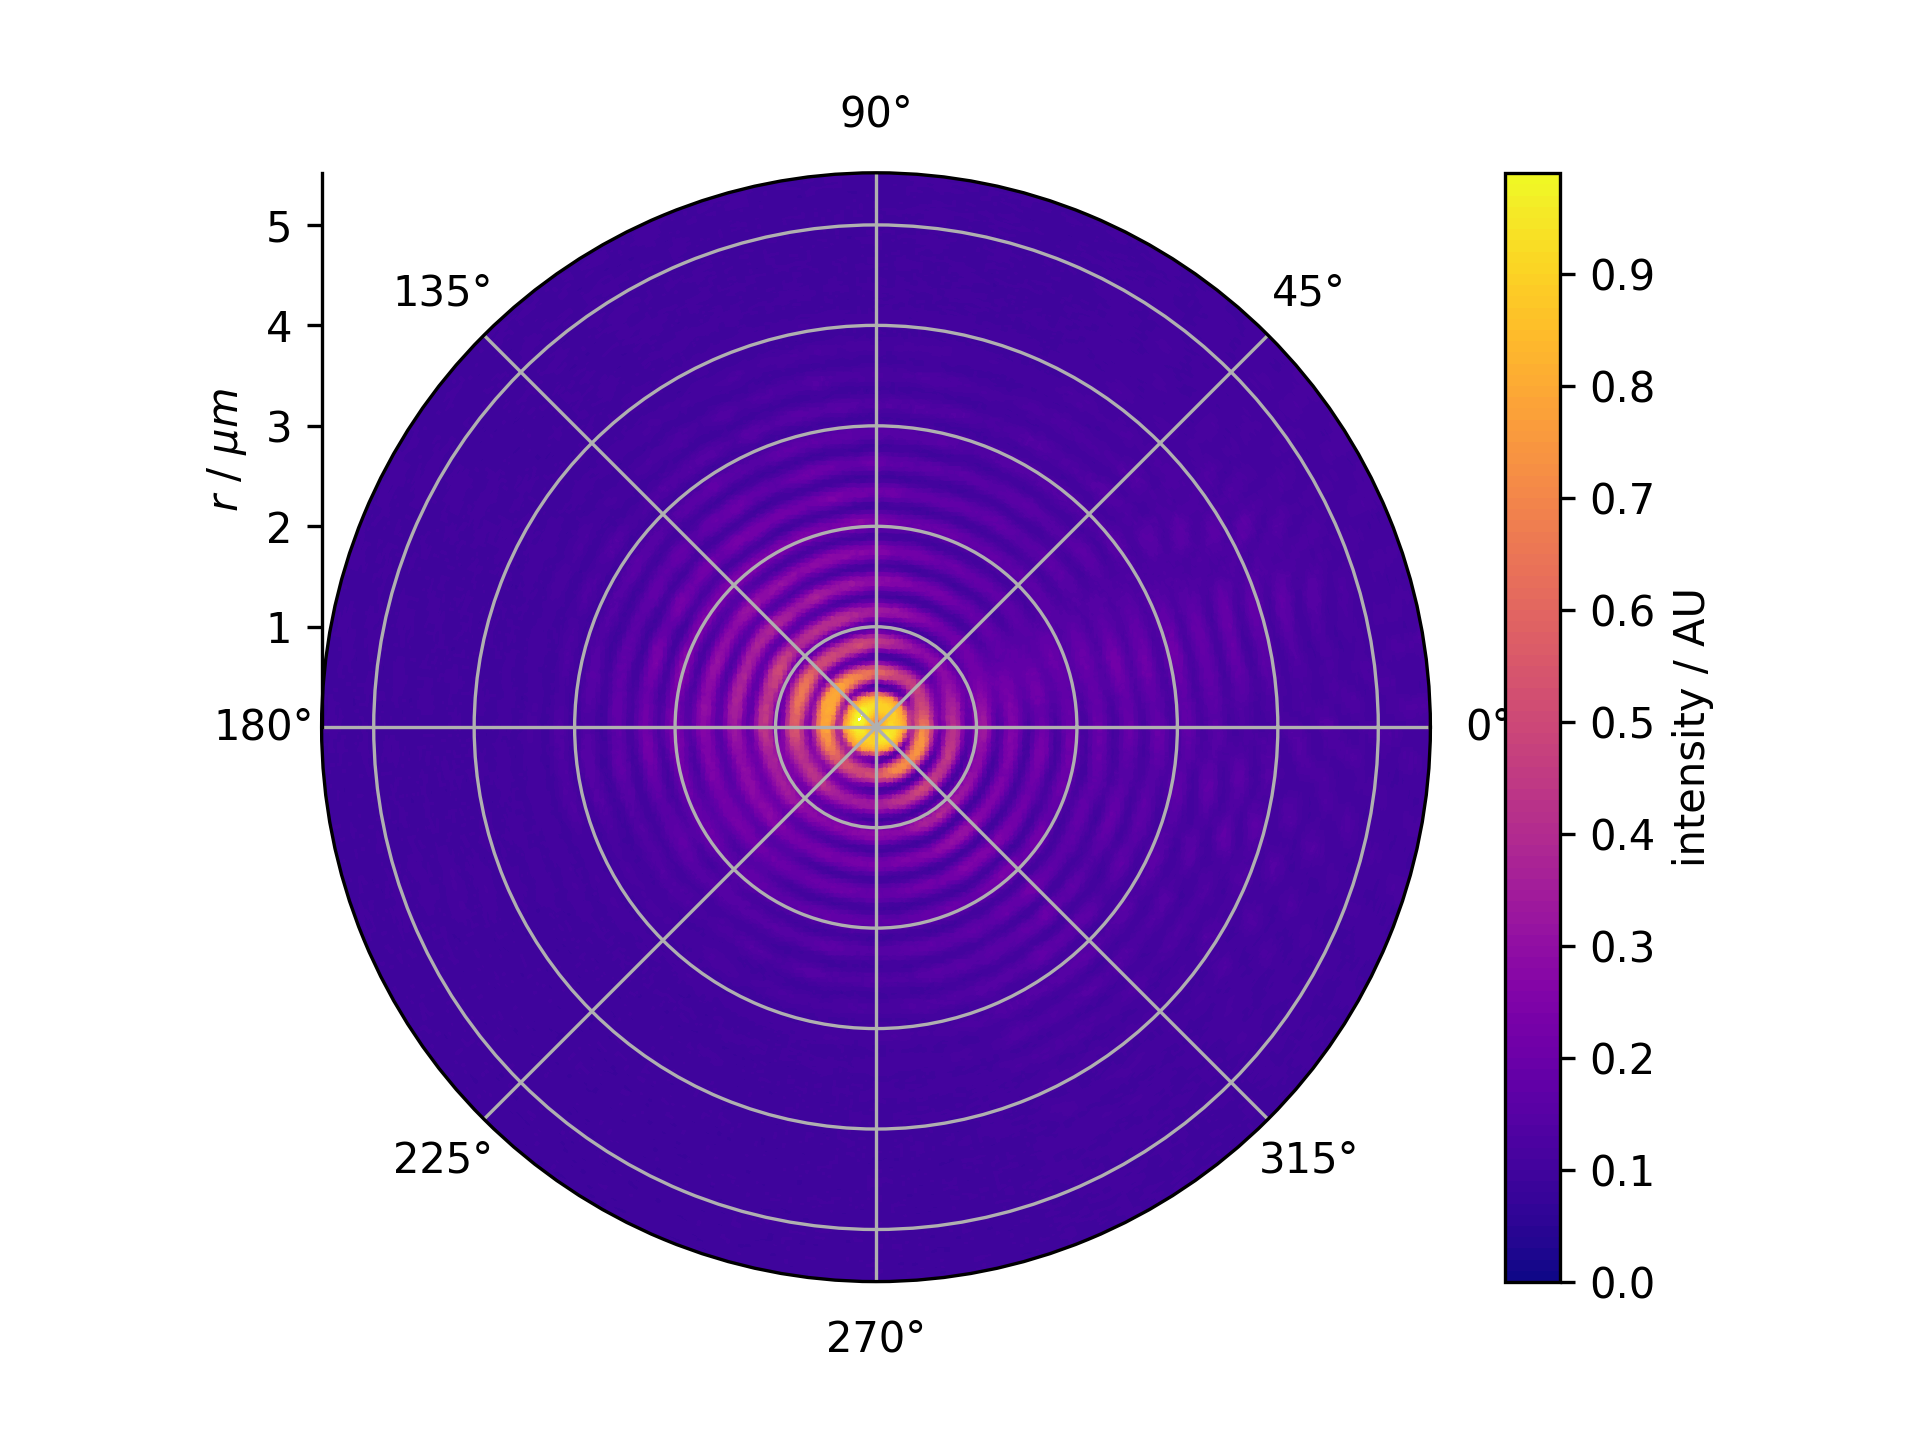
\includegraphics[width=\textwidth]{figures/fp/fp_135.png}
			\caption{$I_r(|\vec{r}|, \phi, \alpha_{\lambda /4} = 135^\circ)$}
			\label{fig:raw_fp_135}
		\end{subfigure}
		\begin{subfigure}[b]{0.5\textwidth}
			\centering
			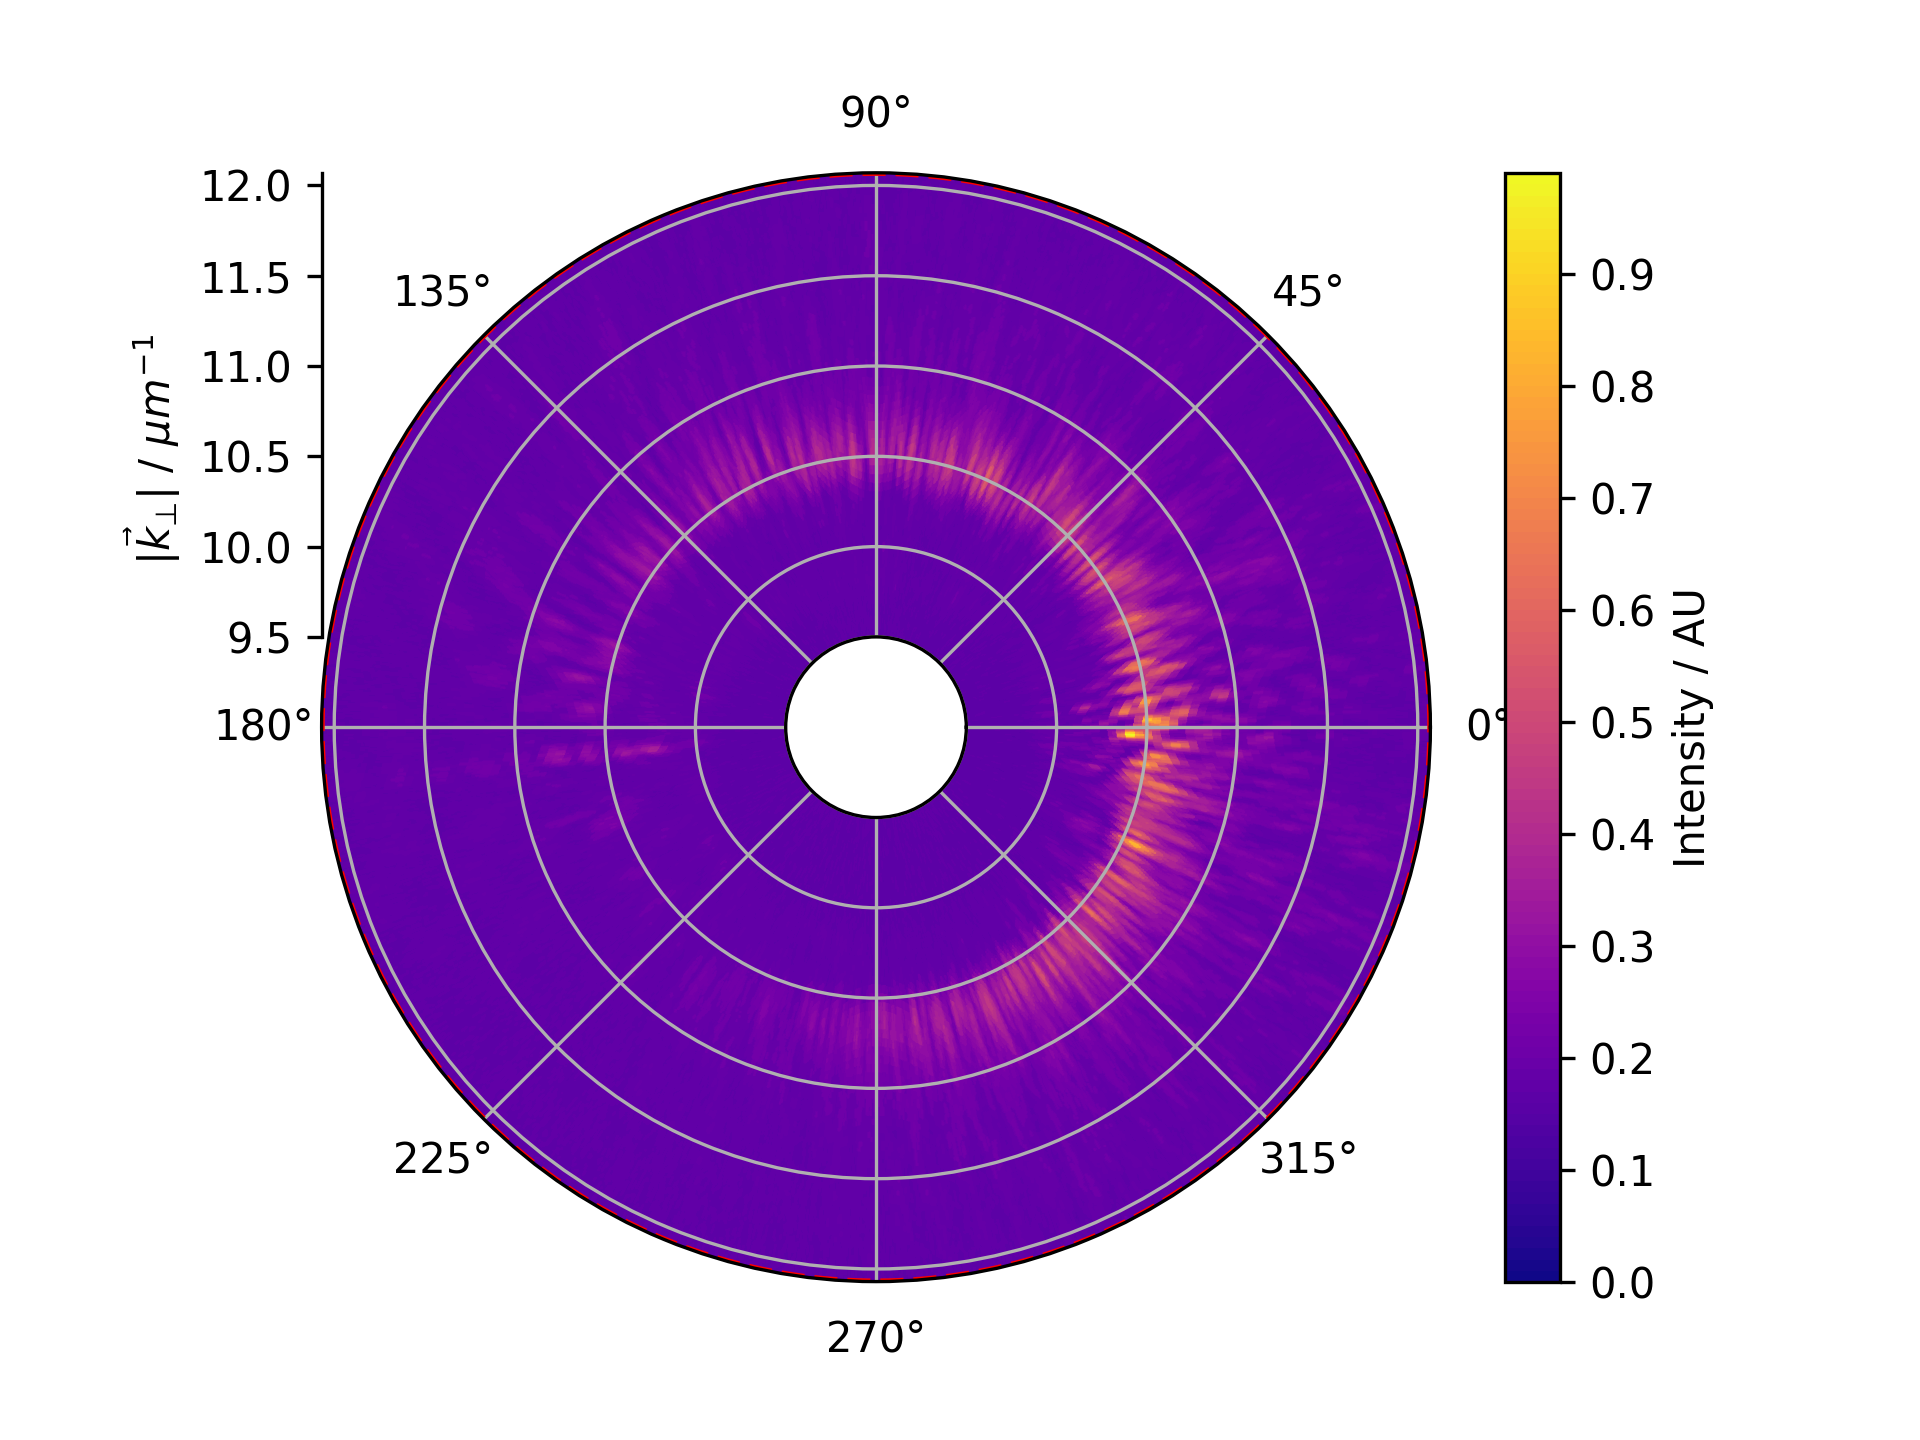
\includegraphics[width=\textwidth]{figures/spin_hall/polar/polar_135.png}
			\caption{$I_k(|\vec{k}_\perp|, \phi, \alpha_{\lambda /4}= 135^\circ)$}
			\label{fig:raw_bfp_135}
		\end{subfigure}
		\caption[Rohdaten PSHE]{Die Abbildung zeigt Rohdaten der Leckstrahlung eines SPPs im Ortsraum (\subref{fig:raw_fp_45}, \subref{fig:raw_fp_135}) und im Impulsraum (\subref{fig:raw_bfp_45}, \subref{fig:raw_bfp_135}). Der direkt transmittierte Strahl wurde dabei mit dem BB aus der Abbildung gefiltert. Die Messungen \subref{fig:raw_fp_45}, \subref{fig:raw_bfp_45} sind dabei mit einer Orientierung der $\lambda / 4$-Platte von $\alpha_{\lambda/4} = 45^\circ$ aufgenommen und \subref{fig:raw_fp_135}, \subref{fig:raw_bfp_135} mit $\alpha_{\lambda/4} = 135^\circ$. Diese Orientierungen sorgen für eine links- bzw. rechts-zirkulare Polarisation des Anregungslasers.}
		\label{fig:measure_pshe_raw}			
	\end{figure}
	\paragraph{Ortsraum}
	In den Rohdaten ist im Ortsbild in Rückwärtsrichtung bezüglich der Einfallsrichtung des Anregungslasers bereits eine leichte Asymmetrie zu beobachten: Die Intensität der Anregung ist in Abbildung \ref{fig:raw_fp_45} zwischen $90^\circ$ und $180^\circ$ größer als zwischen $180^\circ$ und $270^\circ$. Bei Wechsel des Drehsinns der Polarisation des Anregungslaser (Abbildung \ref{fig:raw_fp_135}) invertiert diese Asymmetrie ihr Vorzeichen. In Vorwärtsrichtung ist bemerkenswerterweise auch eine Asymmetrie zu beobachten, die zur Asymmetrie in Rückwärtsrichtung entgegengesetzt ist: In Abbildung \ref{fig:raw_fp_45} ist die gemessene Intensität zwischen $0^\circ$ und $90^\circ$ größer als zwischen $270^\circ$ und $360^\circ$. Auch diese Asymmetrie invertiert bei Wechsel des Drehsinns der Polarisation ihr Vorzeichen.
	\paragraph{Impulsraum} 
	In den Rohdaten des Impulsraumes ist in Rückwärtsrichtung ein äquivalentes Verhalten zu dem Verhalten der Anregung im Ortsraum zu erkennen. In Vorwärtsrichtung ist in den Rohdaten des Impulsraumes hingegen keine deutliche Asymmetrie zu beobachten.
	\FloatBarrier
	\subsubsection{Differenz- und Integrationsdaten}
		Um die Asymmetrie bei Anregung mit zirkular polarisierter Strahlung im Detail zu untersuchen, wurde ein Differenzbild zwischen den Intensitäten, die bei links- und rechts-zirkular polarisierter Anregungsstrahlung gemessen worden sind, errechnet. Diese Differenzdaten wurden sowohl für die Messung im Ortsraum als auch für die Messung im Impulsraum bestimmt.			
		\paragraph{Ortsraum}
		Im Ortsraum lässt sich die relative Intensitätsdifferenz zwischen der Leckstrahlung, die durch die Anregung mit links- und rechts-zirkular polarisierter Strahlung entsteht, durch folgenden Ausdruck berechnen:
		\begin{equation}
		 	\label{eq:diff_measure}
			D_r\left(|\vec{r}|, \Phi\right) := \dfrac{I_r(|\vec{r}|, \phi, \alpha_{\lambda /4} = 45^\circ) - I_r(|\vec{r}|, \phi, \alpha_{\lambda /4} = 135^\circ)}{I_r(|\vec{r}|, \phi, \alpha_{\lambda /4} = 45^\circ) + I_r(|\vec{r}|, \phi, \alpha_{\lambda /4} = 135^\circ)}
		\end{equation} 
		 Diese relative Intensitätsdifferenz im Ortsraum ist in Abbildung \ref{fig:diff_fp_45_135} dargestellt. In dieser Darstellung ist zu erkennen, dass die relative Intensitätsdifferenz in radialer Richtung eine Modulation mit der gleichen Raumfrequenz wie die Rohdaten zeigt. Auf konzentrischen Kreisen mit geringer Intensität im Ursprungssignal treten im Differenzbild negative Werte auf, und auf konzentrischen Kreisen mit hoher Intensität im Ursprungssignal treten positive Werte im Differenzbild auf. Die Modulation der Differenz in polarer Richtung entsteht nur durch ein Verringern einer der beiden oben beschriebenen Differenzen, nicht jedoch durch einen Vorzeichenwechsel. Für dieses Verhalten konnte im Rahmen dieser Arbeit keine endgültige Erklärung gefunden werden. Die radiale Modulation der Intensität im Ortsbild der Leckstrahlung entsteht durch unterschiedliche Effekte, die nur durch umfangreiche Simulationen untersucht werden können. Zum einen entsteht ein räumlich moduliertes Signal durch die scharfe Begrenzung der Raumfrequenzen durch die Numerische Apertur. Diese Signalmodulation wird von einer Modulation, die direkt durch das SPP entsteht, überlagert. Aus diesen beiden Modulationen entsteht eine Schwebung die zu dem beobachteten Signal führt. In \cite{Hohenau.2011} wird die Bildentstehung in einem LRM mit linear polarisiertem Licht sehr detailliert erläutert und simuliert. Dort wird allerdings nicht auf den Einfluss von zirkularer Polarisation auf die Bildentstehung eingegangen.
		 
		 Um die Asymmetrie der Anregung bezüglich der Einfallsebene des Lasers in Abhängigkeit der Polarisation des Lasers zu charakterisieren, wurden zwei Bereiche im Ortsraum ausgewählt, über die die Intensität integriert wurde. Diese Integrationsbereiche wurden symmetrisch bezüglich der horizontalen Einfallsebene des Lasers gewählt:		 
		 \begin{align}
		 	P_{r, \mathrm{Oben}}(\alpha_{\lambda/4}) &:= \int_{0}^{r_\mathrm{max}}r \, \mathrm{d}r \int_{\phi_\mathrm{min}}^{\phi_\mathrm{max}} \mathrm{d}\phi I_r(r, \phi, \alpha_{\lambda /4}) \\
		 	\nonumber
		 	P_{r, \mathrm{Unten}}(\alpha_{\lambda/4}) &:= \int_{0}^{r_\mathrm{max}}r \, \mathrm{d}r \int_{360^\circ -\phi_\mathrm{max}}^{360^\circ - \phi_\mathrm{min}} \mathrm{d}\phi I_r(r, \phi, \alpha_{\lambda/4})		 	
		 \end{align}
	 
		 \begin{align}
		 	\label{eq:relative_power}
		 	P_{r, \mathrm{relativ}, \mathrm{Oben}}(\alpha_{\lambda/4}) &:= 	\dfrac{P_{r, \mathrm{Oben}}(\alpha_{\lambda/4})}{P_{r, \mathrm{Oben}}(\alpha_{\lambda/4}) + P_{r, \mathrm{Unten}}(\alpha_{\lambda/4})} \\
		 	\nonumber
		 	P_{r, \mathrm{relativ}, \mathrm{Unten}}(\alpha_{\lambda/4}) &:= 	\dfrac{P_{r, \mathrm{Unten}}(\alpha_{\lambda/4})}{P_{r, \mathrm{Oben}}(\alpha_{\lambda/4}) + P_{r, \mathrm{Unten}}(\alpha_{\lambda/4})}	 	
		 \end{align}
	 	Hierbei ist $r_\mathrm{max}$ die Begrenzung der Integrationsbereiche in radialer Richtung. Die Winkel $\phi_\mathrm{min} < \phi_\mathrm{max}$ legen die beiden Integrationsbereiche in polarer
	 	 Richtung fest. Diese über eine Fläche integrierte Intensität ist eine Leistung. Die Integration wurde für alle Orientierungen des $\lambda/4$-Plättchens durchgeführt. Die Leistungen des oberen und unteren SPP wurde mit den Beziehungen \eqref{eq:relative_power} auf die Summe der beiden Leistungen normiert. Das Ergebnis dieser Auswertung ist in den Abbildungen \ref{fig:int_fp_45_135}, \subref{fig:int_fp_45_135_mid}, \subref{fig:int_fp_45_135_front} für unterschiedliche Kombinationen von $\phi_\mathrm{min}$ und $\phi_\mathrm{max}$ dargestellt. Die Integrationsbereiche sind dabei jeweils in  \ref{fig:diff_fp_45_135}, \subref{fig:diff_fp_45_135_mid}, \subref{fig:diff_fp_45_135_front} markiert.		 
		\begin{figure}		
			\begin{subfigure}[b]{0.5\textwidth}
				\centering
				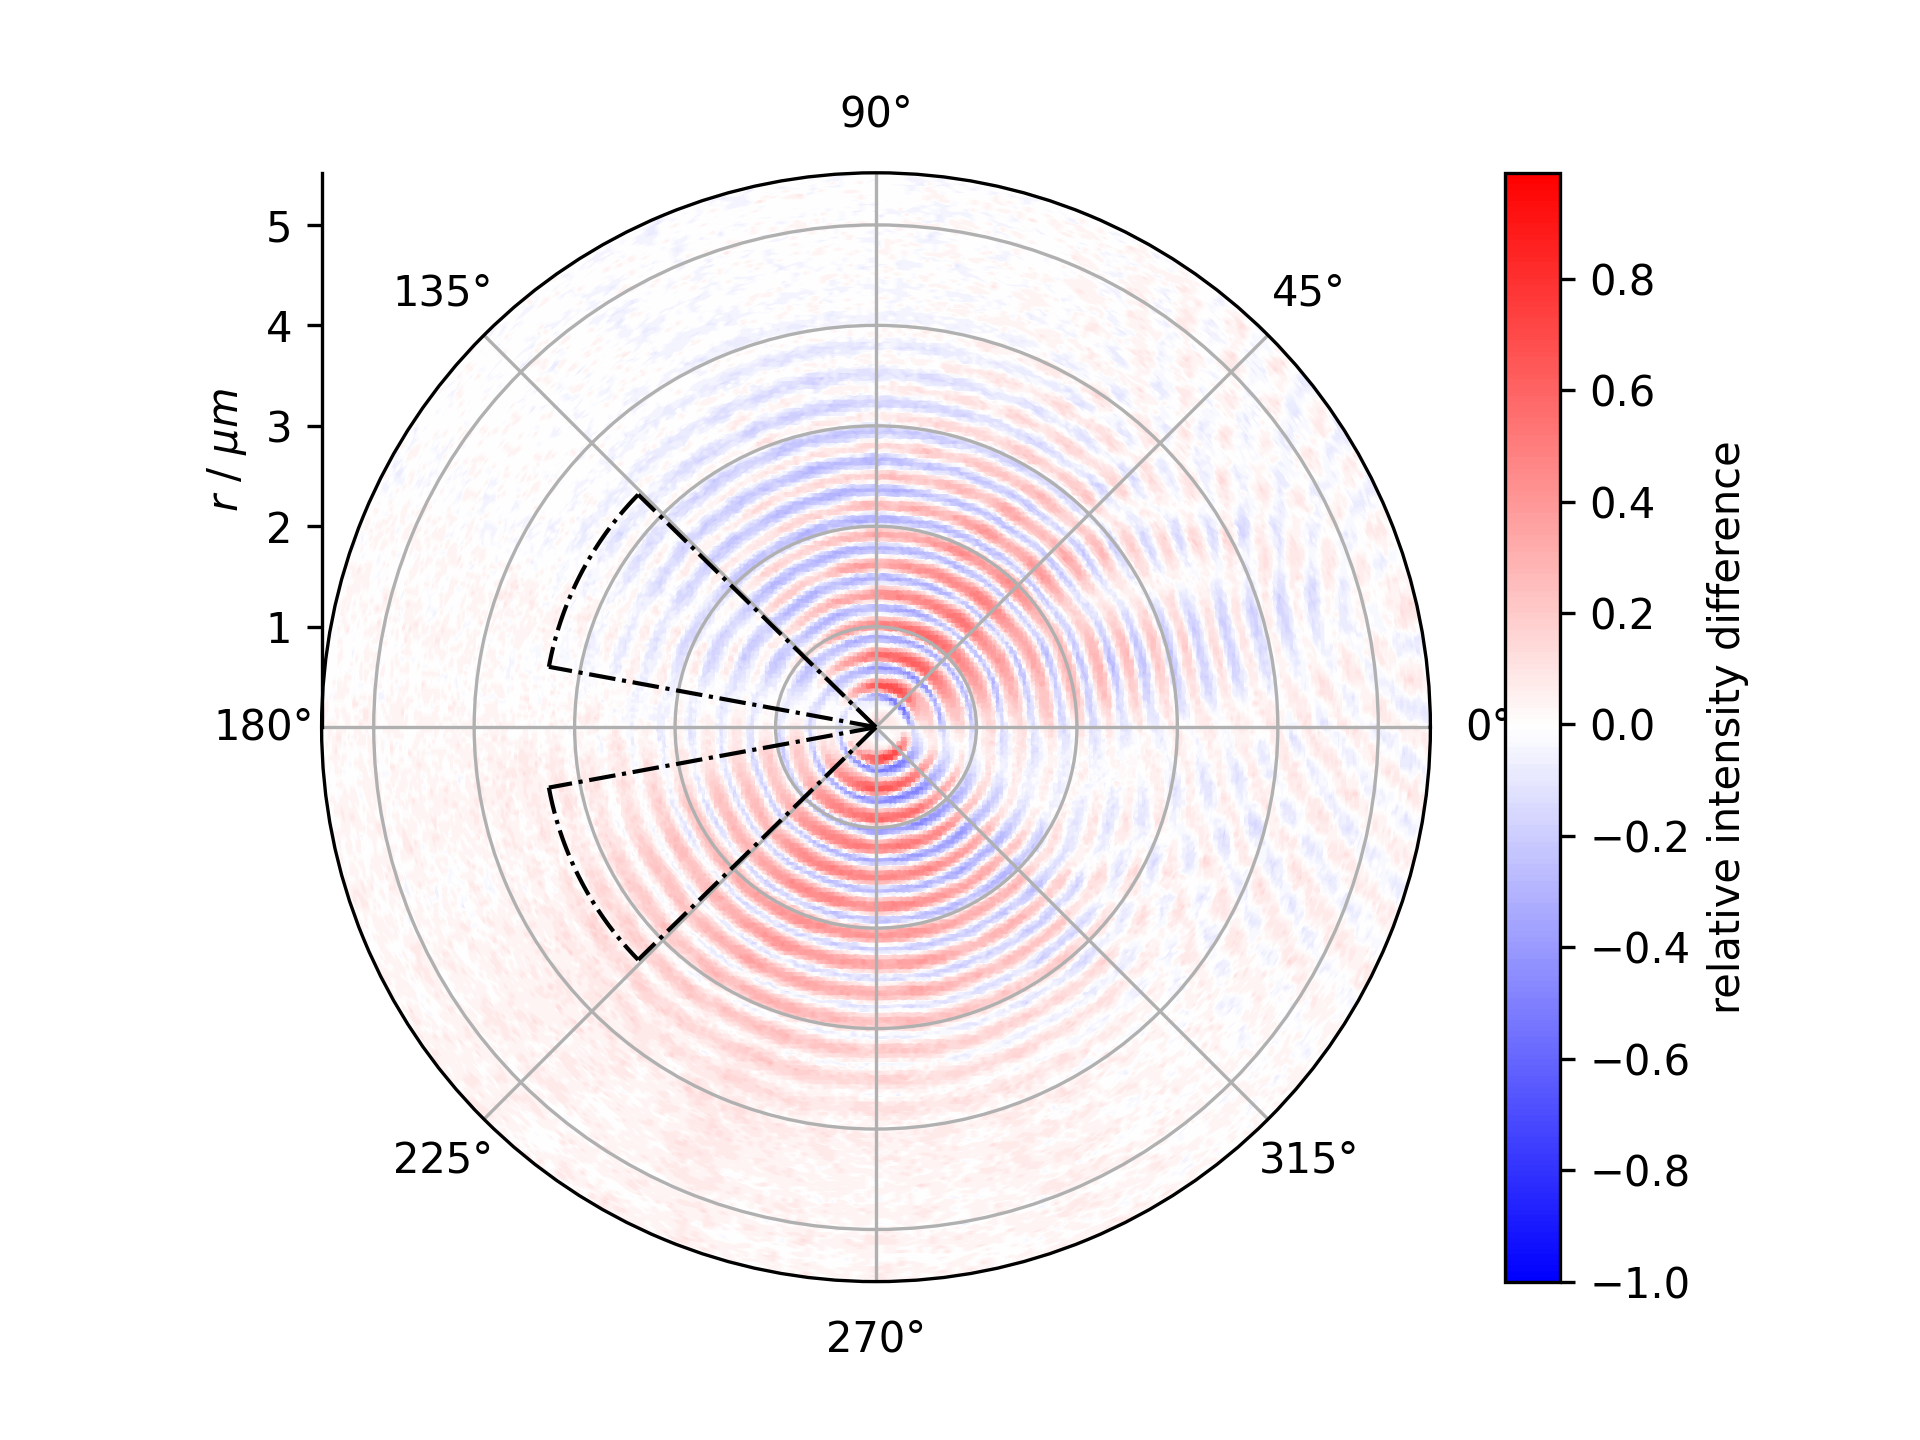
\includegraphics[width=\textwidth]{figures/fp/fp_back.png}
				\caption{	$D_r\left(|\vec{r}|, \Phi\right)$}
				\label{fig:diff_fp_45_135}
			\end{subfigure}
			\hfill
			\begin{subfigure}[b]{0.49\textwidth}
				\centering
				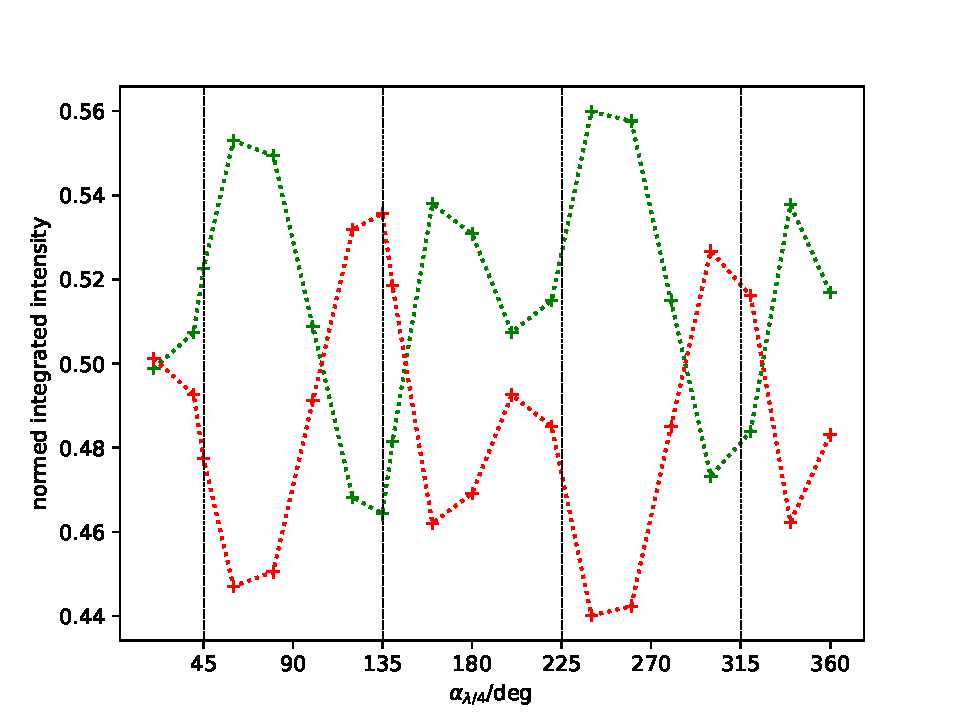
\includegraphics[width=\textwidth]{figures/fp/fp_back_int.pdf}
				\caption{$\phi_\mathrm{min} =135^\circ, \phi_\mathrm{max}=170^\circ$}
				\label{fig:int_fp_45_135}
			\end{subfigure}
			
			\begin{subfigure}[b]{0.5\textwidth}
				\centering
				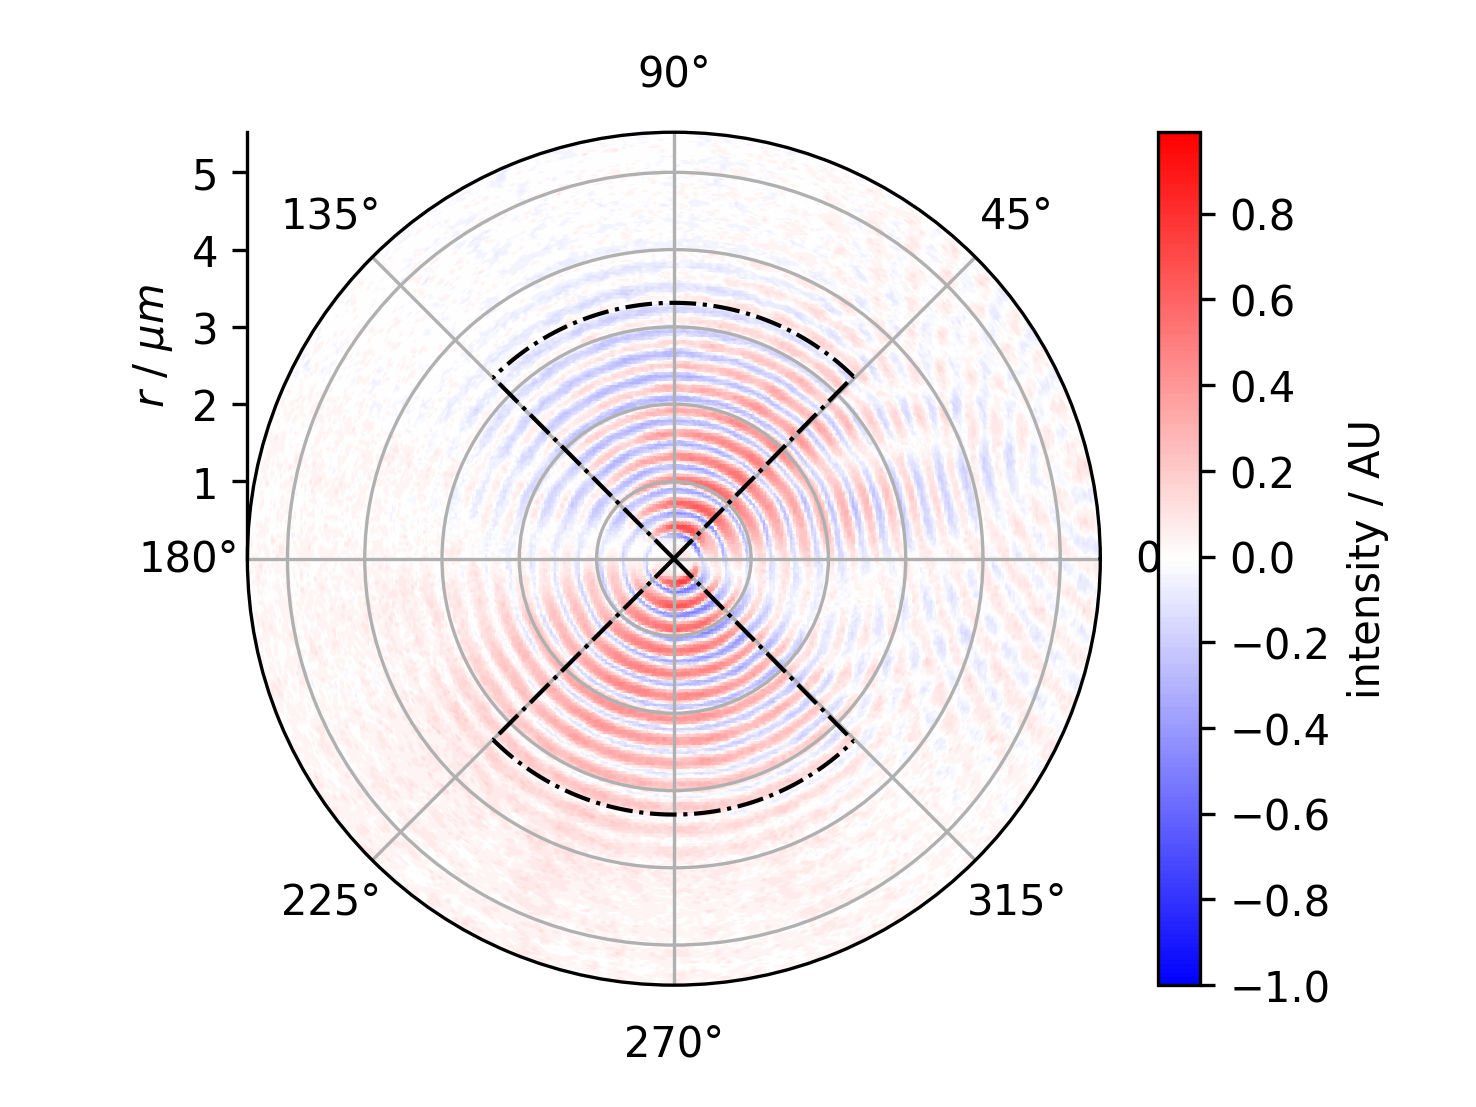
\includegraphics[width=\textwidth]{figures/fp/fp_mid.png}
				\caption{$D_r\left(|\vec{r}|, \Phi\right)$}
				\label{fig:diff_fp_45_135_mid}
			\end{subfigure}
			\hfill
			\begin{subfigure}[b]{0.49\textwidth}
				\centering
				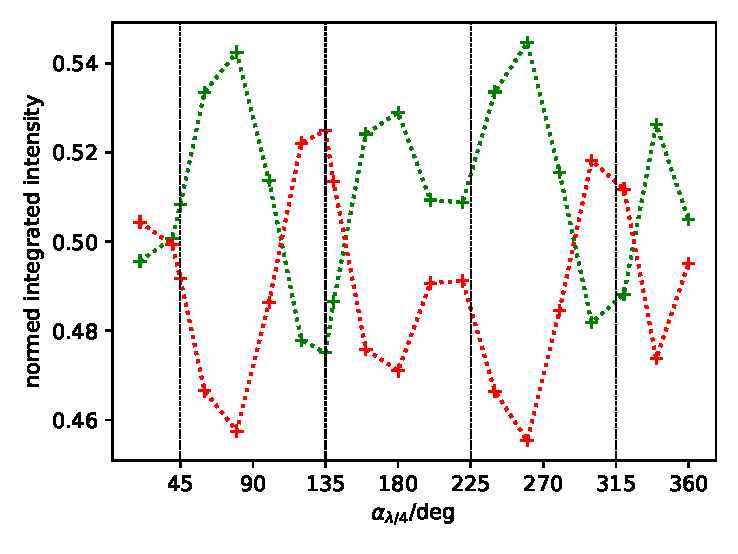
\includegraphics[width=\textwidth]{figures/fp/fp_mid_int.pdf}
				\caption{ $\phi_\mathrm{min} =45^\circ, \phi_\mathrm{max}=135^\circ$}
				\label{fig:int_fp_45_135_mid}
			\end{subfigure}
			
			\begin{subfigure}[b]{0.5\textwidth}
				\centering
				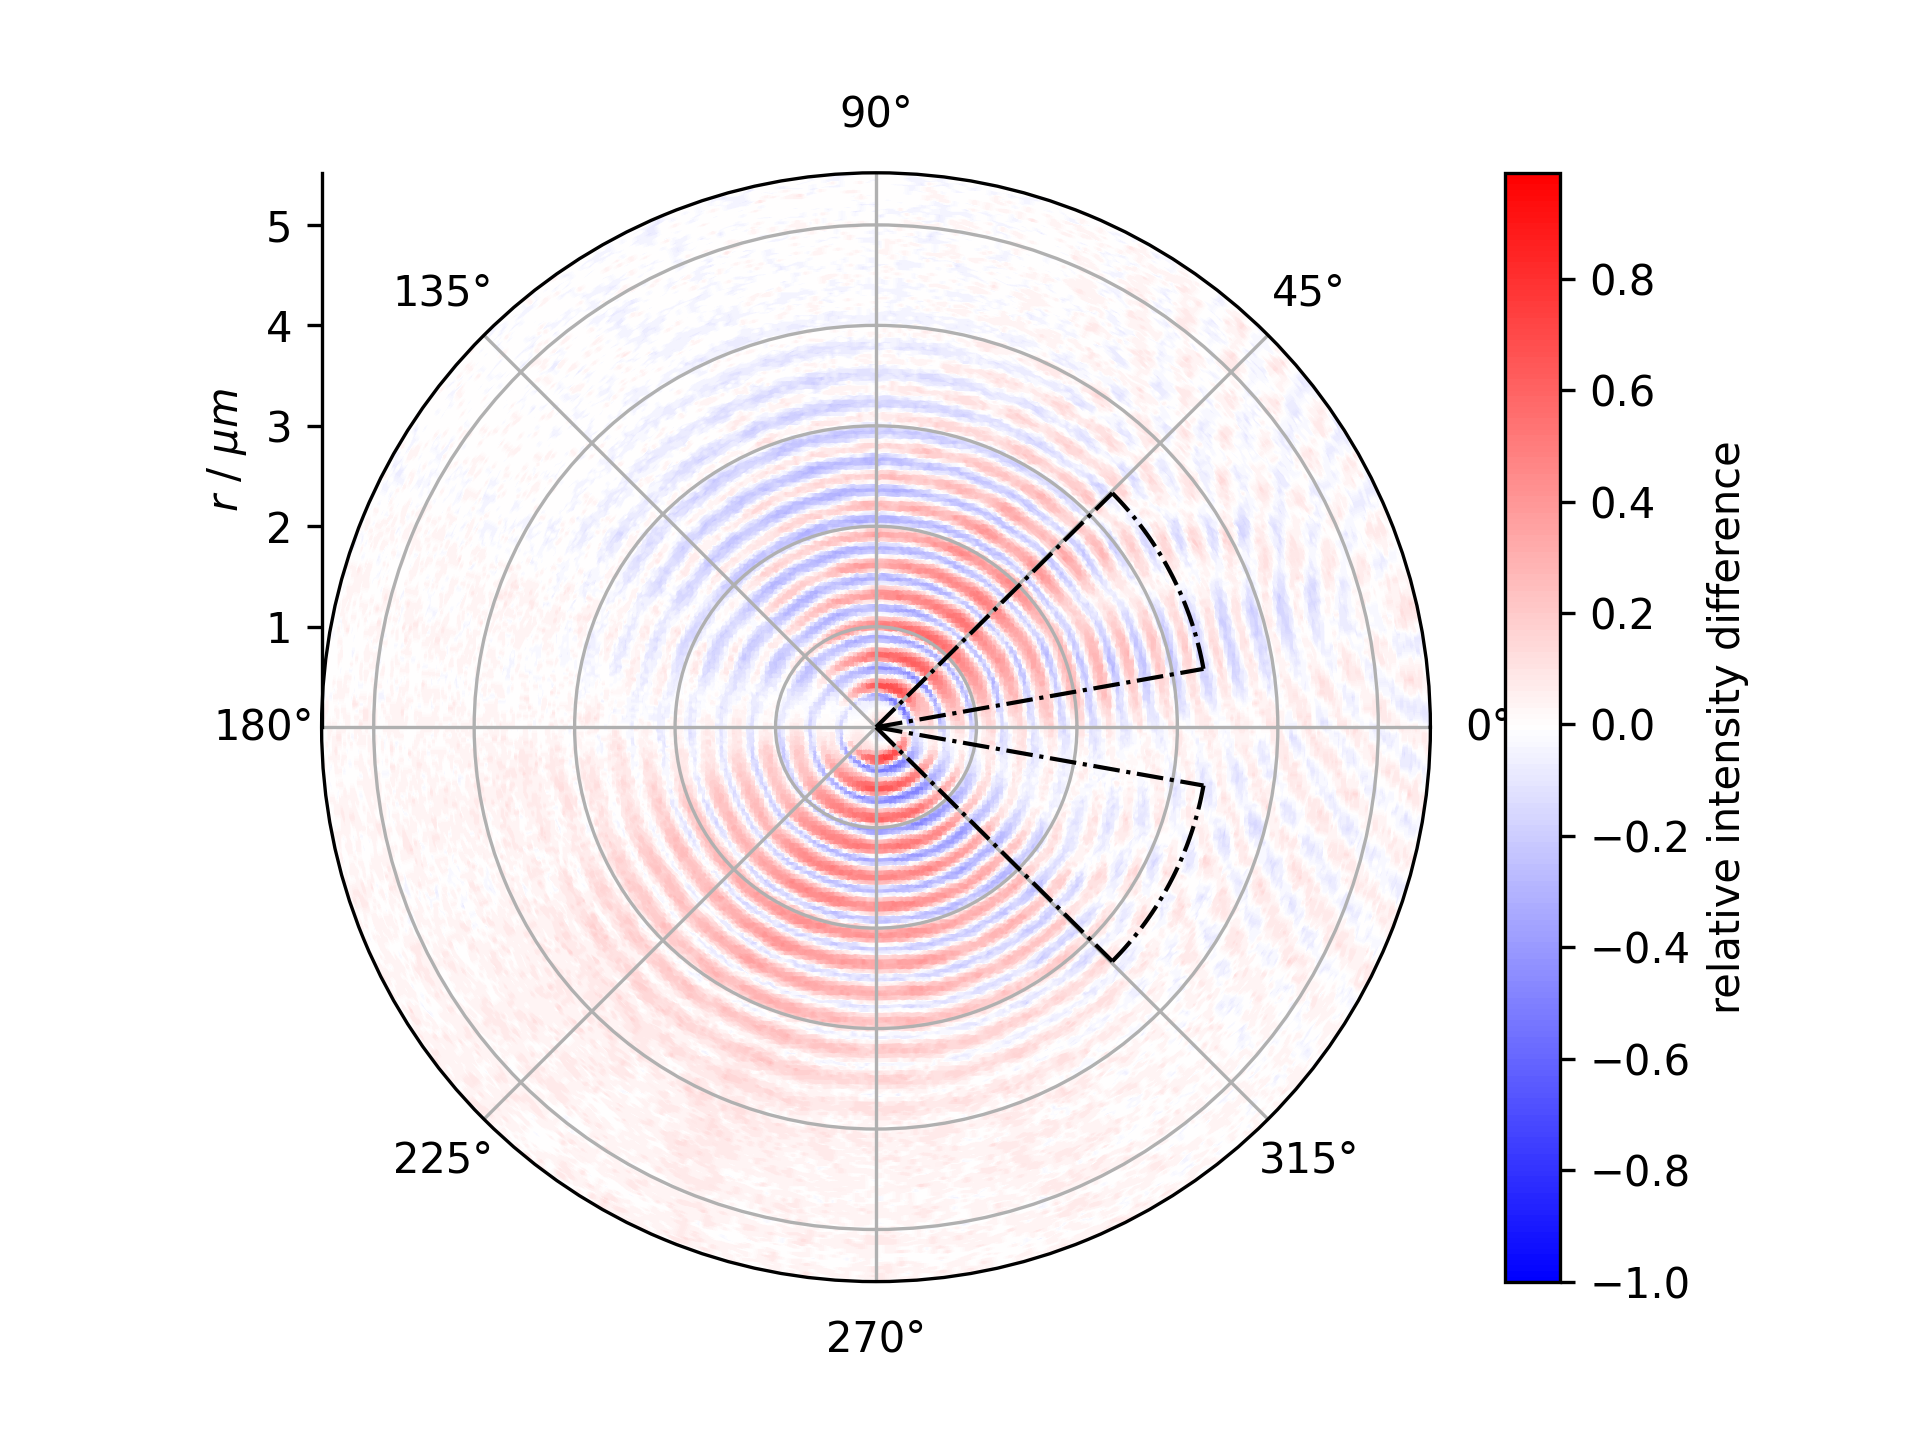
\includegraphics[width=\textwidth]{figures/fp/fp_forw.png}
				\caption{$D_r\left(|\vec{r}|, \Phi\right)$}
				\label{fig:diff_fp_45_135_front}
			\end{subfigure}
			\hfill
			\begin{subfigure}[b]{0.49\textwidth}
				\centering
				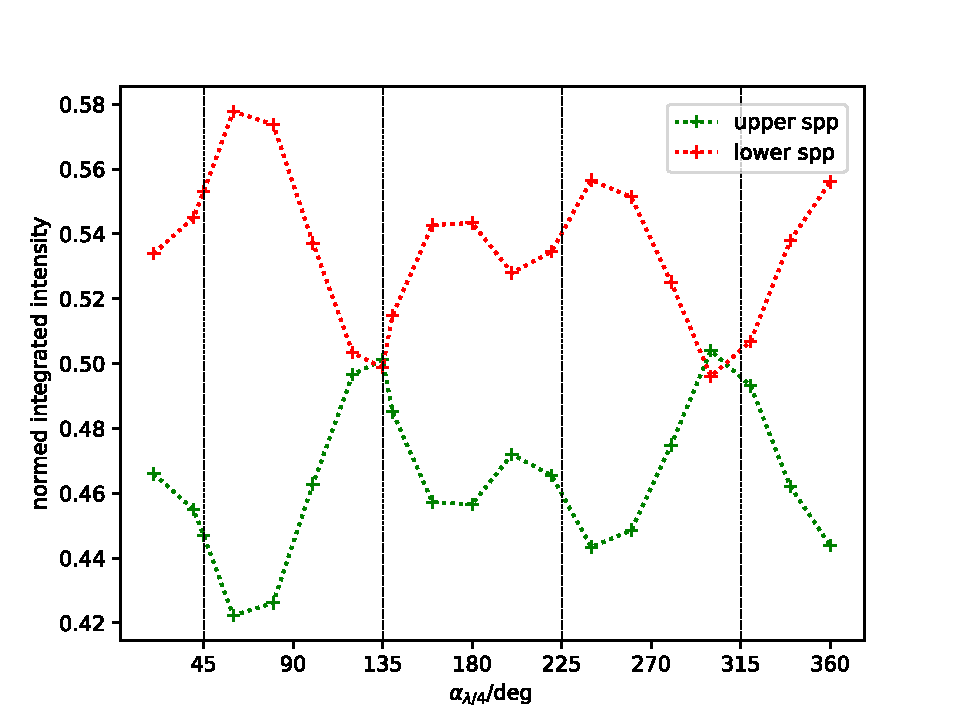
\includegraphics[width=\textwidth]{figures/fp/fp_forw_int.pdf}
				\caption{ $\phi_\mathrm{min} =10^\circ, \phi_\mathrm{max}=45^\circ$}
				\label{fig:int_fp_45_135_front}
			\end{subfigure}
			\caption[Differenz- und Integrationsdaten PSHE Ortsraum]{Die Abbildungen \subref{fig:diff_fp_45_135}, \subref{fig:diff_fp_45_135_mid}, \subref{fig:diff_fp_45_135_front} zeigen die nach \eqref{eq:diff_measure} berechnete relative Differenz der Intensitäten im Ortsraum zwischen links- bzw. rechts-zirkular polarisierter Anregungsstrahlung. Diese Abbildungen unterscheiden sich nur in den markierten Integrationsbereichen. Die Abbildungen \subref{fig:int_fp_45_135}, \subref{fig:int_fp_45_135_mid}, \subref{fig:int_fp_45_135_front} zeigen jeweils die mit \eqref{eq:relative_power} über die zugehörigen markierten Bereiche integrierte Intensität normiert auf die Summe der Intensitäten beider Bereiche in Abhängigkeit der Orientierung des $\lambda/4$-Plättchens, also $P_{r, \mathrm{relativ}, \mathrm{Oben}}(\alpha_{\lambda/4})$ und $P_{r, \mathrm{relativ}, \mathrm{Unten}}(\alpha_{\lambda/4})$. Die vertikalen Linien markieren dabei die Orientierung des $\lambda/4$-Plättchens $\alpha_{\lambda/4}$, bei denen zirkulare Polarisation auftritt.}
			\label{fig:spin_hall_measure_diff_fp}
		\end{figure}
		\subparagraph{Analyse}
			\begin{itemize}
				\item In Rückwärtsrichtung (Abbildung \ref{fig:diff_fp_45_135}, \subref{fig:int_fp_45_135} mit $\phi_\mathrm{min} =135^\circ, \phi_\mathrm{max}=170^\circ$) konnte im Ortsraum die für den PSHE erwartete Asymmetrie beobachtet werden. Bei zirkularer Polarisation ($\alpha_{\lambda/4} \in \{45^\circ, 135^\circ, 225^\circ, 315^\circ\}$, in der Abbildung \ref{fig:int_fp_45_135} durch senkrechte Linien gekennzeichnet) ist jeweils eine Asymmetrie in Bezug auf die Einfallsebene zu erkennen. Diese Asymmetrie wechselt bei Umkehr des Drehsinns der zirkularen Polarisation wie erwartet ihre Orientierung. Allerdings liegen die Maxima dieser Asymmetrie jeweils etwas zur zirkularen Polarisation verschoben. Es ist außerdem auffällig, dass in den Intervallen $\alpha_{\lambda/4} \in [135^\circ,225^\circ]$ und $\alpha_{\lambda/4} \in [315^\circ, 225^\circ]$ jeweils ein weiteres Maximum in der Asymmetrie auftritt. Bei $\alpha_{\lambda/4} \in \{0^\circ, 90^\circ, 180^\circ, 270^\circ\}$ ist die Anregungsstrahlung linear polarisiert. Der elektrische Feldvektor ist dabei parallel zur Einfallsebene orientiert. Daher sollte bei diesen Orientierungen keine Asymmetrie auftreten.
				\item Senkrecht zur Einfallsebene (Abbildung \ref{fig:diff_fp_45_135_mid}, \subref{fig:int_fp_45_135_mid} mit $\phi_\mathrm{min} =45^\circ, \phi_\mathrm{max}=135^\circ$) ist ein sehr ähnliches Verhalten wie in Rückwärtsrichtung zu beobachten. Bei zirkularer Polarisation ist weiterhin eine mit dem Drehsinn der Polarisation alternierende Asymmetrie zwischen oberen und unteren SPP zu erkennen. Allerdings ist diese Asymmetrie bei $\alpha_{\lambda/4}=45^\circ$ vergleichsweise klein. Senkrecht zur Einfallsebene tritt ebenfalls jeweils ein weiteres Maximum in den Intervallen $\alpha_{\lambda/4} \in [135^\circ,225^\circ]$ und $\alpha_{\lambda/4} \in [315^\circ, 225^\circ]$ auf.
				\item
				In Vorwärtsrichtung (Abbildung \ref{fig:diff_fp_45_135_front}, \subref{fig:int_fp_45_135_front} mit  $\phi_\mathrm{min} =10^\circ, \phi_\mathrm{max}=45^\circ$) ist bemerkenswerterweise eine zu den beiden vorangegangenen Richtungen invertierte Modulation der Intensitäten zu erkennen. Während die Leistung des oberen SPP bei der Integration in Rückwärtsrichtung und senkrecht zur Ausbreitungsrichtung jeweils bei $\alpha_{\lambda /4} \in \{45^\circ, 225^\circ\}$ ein Maximum hatte, liegen bei der Integration in Vorwärtsrichtung bei diesen Orientierungen die Minima.
			\end{itemize}
		\paragraph{Impulsraum}
		Die oben ausgeführte Auswertung kann analog auch auf die Messdaten des Impulsraumes angewendet werden:
		\begin{equation}
			\label{eq:diff_measure_momentum}
			D_k\left(|\vec{k}_\perp|, \Phi\right) := \dfrac{I_k(|\vec{k}_\perp|, \phi, \alpha_{\lambda /4} = 45^\circ) - I_k(|\vec{k}_\perp|, \phi, \alpha_{\lambda /4} = 135^\circ)}{I_k(|\vec{k}_\perp|, \phi, \alpha_{\lambda /4} = 45^\circ) + I_k(|\vec{k}_\perp|, \phi, \alpha_{\lambda /4} = 135^\circ)}
		\end{equation} 
		\begin{align}
			P_{k, \mathrm{Oben}}(\alpha_{\lambda/4}) &:= \int_{k_\mathrm{min}}^{k_\mathrm{max}}k \, \mathrm{d}k \int_{\phi_\mathrm{min}}^{\phi_\mathrm{max}} \mathrm{d}\phi I_k(k, \phi, \alpha_{\lambda /4}) \\
			\nonumber
			P_{k, \mathrm{Unten}}(\alpha_{\lambda/4}) &:= \int_{k_\mathrm{min}}^{k_\mathrm{max}}k \, \mathrm{d}k \int_{360^\circ -\phi_\mathrm{max}}^{360^\circ - \phi_\mathrm{min}} \mathrm{d}\phi I_k(k, \phi, \alpha_{\lambda/4})		 	
		\end{align}
		
		\begin{align}
			\label{eq:relative_power_momentum}
			P_{k, \mathrm{relativ}, \mathrm{Oben}}(\alpha_{\lambda/4}) &:= 	\dfrac{P_{k, \mathrm{Oben}}(\alpha_{\lambda/4})}{P_{k, \mathrm{Oben}}(\alpha_{\lambda/4}) + P_{k, \mathrm{Unten}}(\alpha_{\lambda/4})} \\
			\nonumber
			P_{k, \mathrm{relativ}, \mathrm{Unten}}(\alpha_{\lambda/4}) &:= 	\dfrac{P_{k, \mathrm{Unten}}(\alpha_{\lambda/4})}{P_{k, \mathrm{Oben}}(\alpha_{\lambda/4}) + P_{k, \mathrm{Unten}}(\alpha_{\lambda/4})}	 	
		\end{align}
		Die Auswertung des Impulsraumes hat gegenüber den Daten des Ortsraumes den Vorteil, dass hier das plasmonische Signal klar von dem Hintergrundsignal getrennt werden kann. Um in die Integration hauptsächlich das plasmonische Signal auf dem Kreisring mit Radius $k = k_\mathrm{SPP} = 10.3\,\mathrm{\mu m}^{-1}$ einfließen zu lassen, wurde die radiale Integration nur zwischen $k_\mathrm{min} = 9.8\,\mathrm{\mu m}^{-1}$ und $k_\mathrm{max} = 10.8\,\mathrm{\mu m}^{-1}$ durchgeführt. Das Differenzbild und die Auswertung der Integrationsbereiche sind in Abbildung \ref{fig:spin_hall_measure} dargestellt.		
		\begin{figure}			
			\begin{subfigure}[b]{0.5\textwidth}
				\centering
				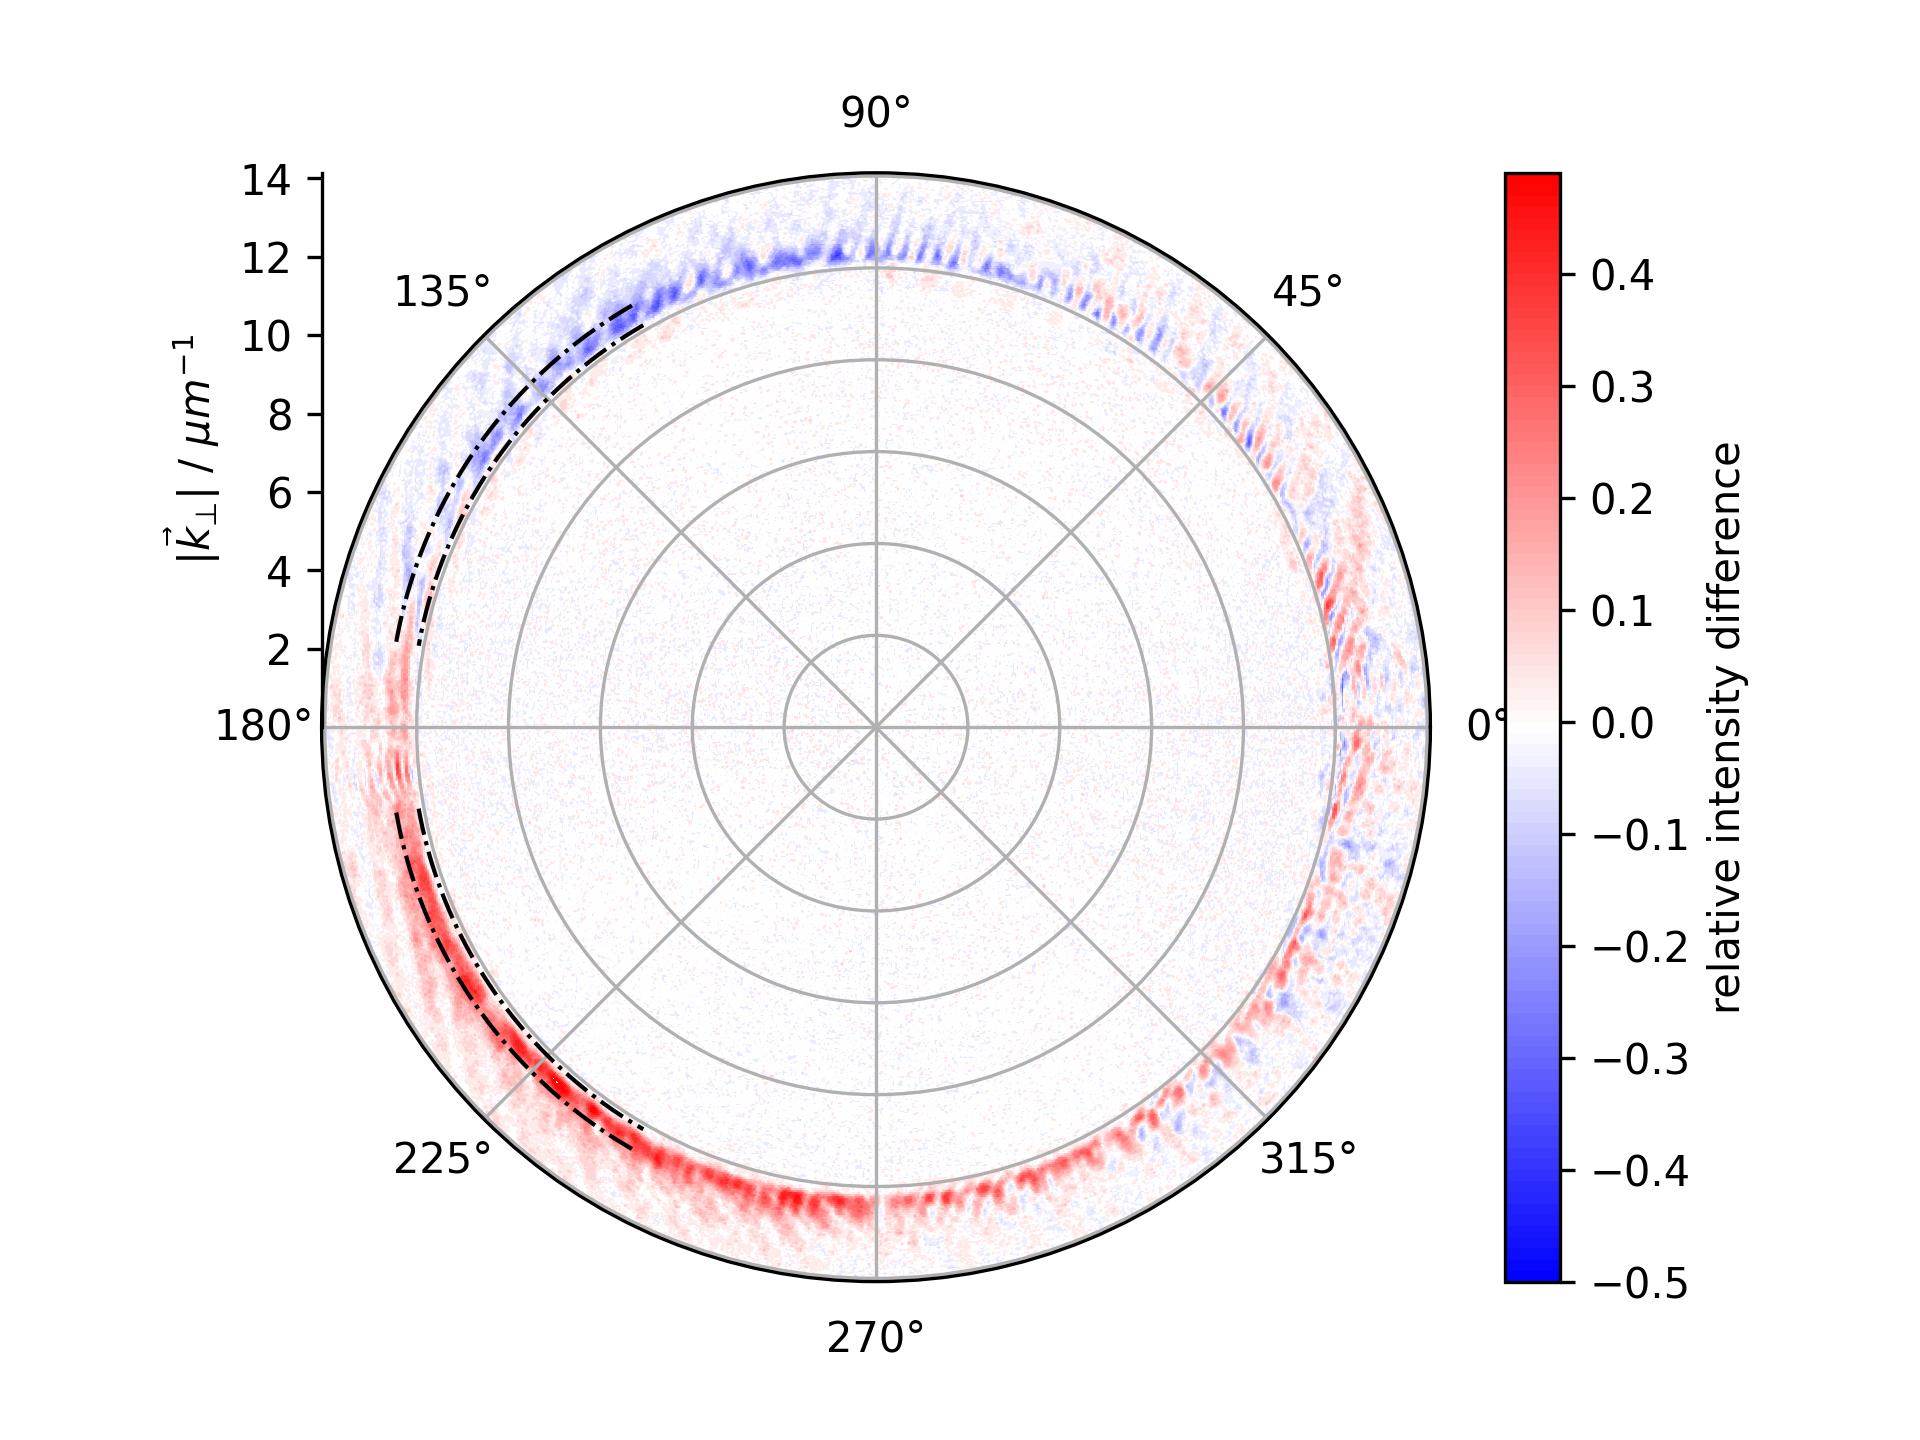
\includegraphics[width=\textwidth]{figures/spin_hall/diff_back.png}
				\caption{$D_k\left(|\vec{k}_\perp|, \Phi\right)$}
				\label{fig:diff_back}
			\end{subfigure}
			\hfill
			\begin{subfigure}[b]{0.49\textwidth}
				\centering
				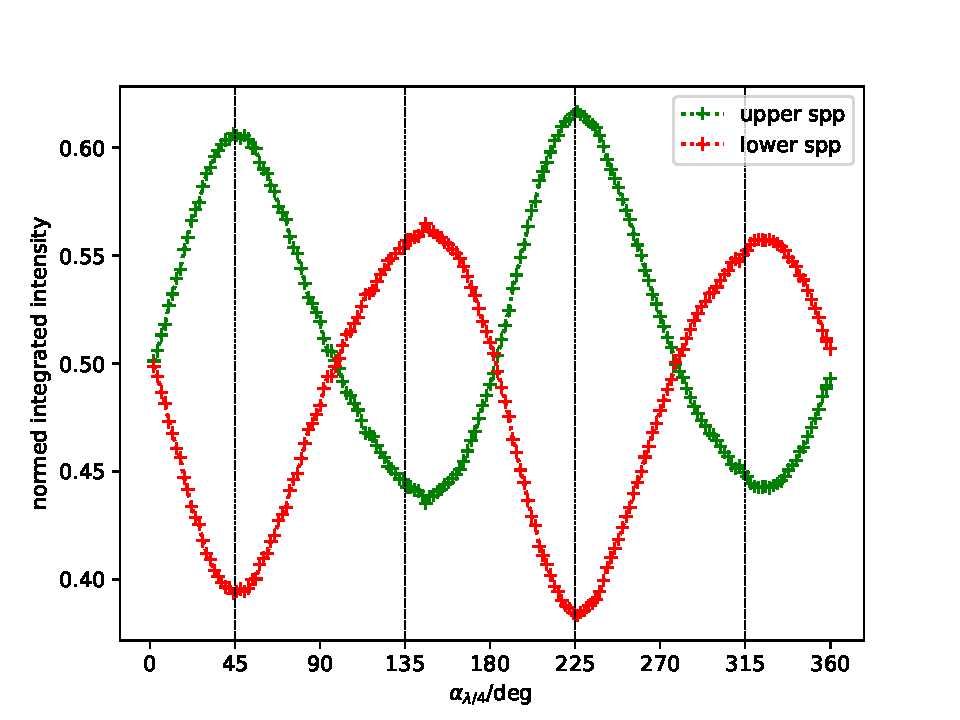
\includegraphics[width=\textwidth]{figures/spin_hall/intensity_back.pdf}
				\caption{$\phi_\mathrm{min} =120^\circ, \phi_\mathrm{max}=170^\circ$}
				\label{fig:intensity_back}
			\end{subfigure}
			
			\begin{subfigure}[b]{0.5\textwidth}
				\centering
				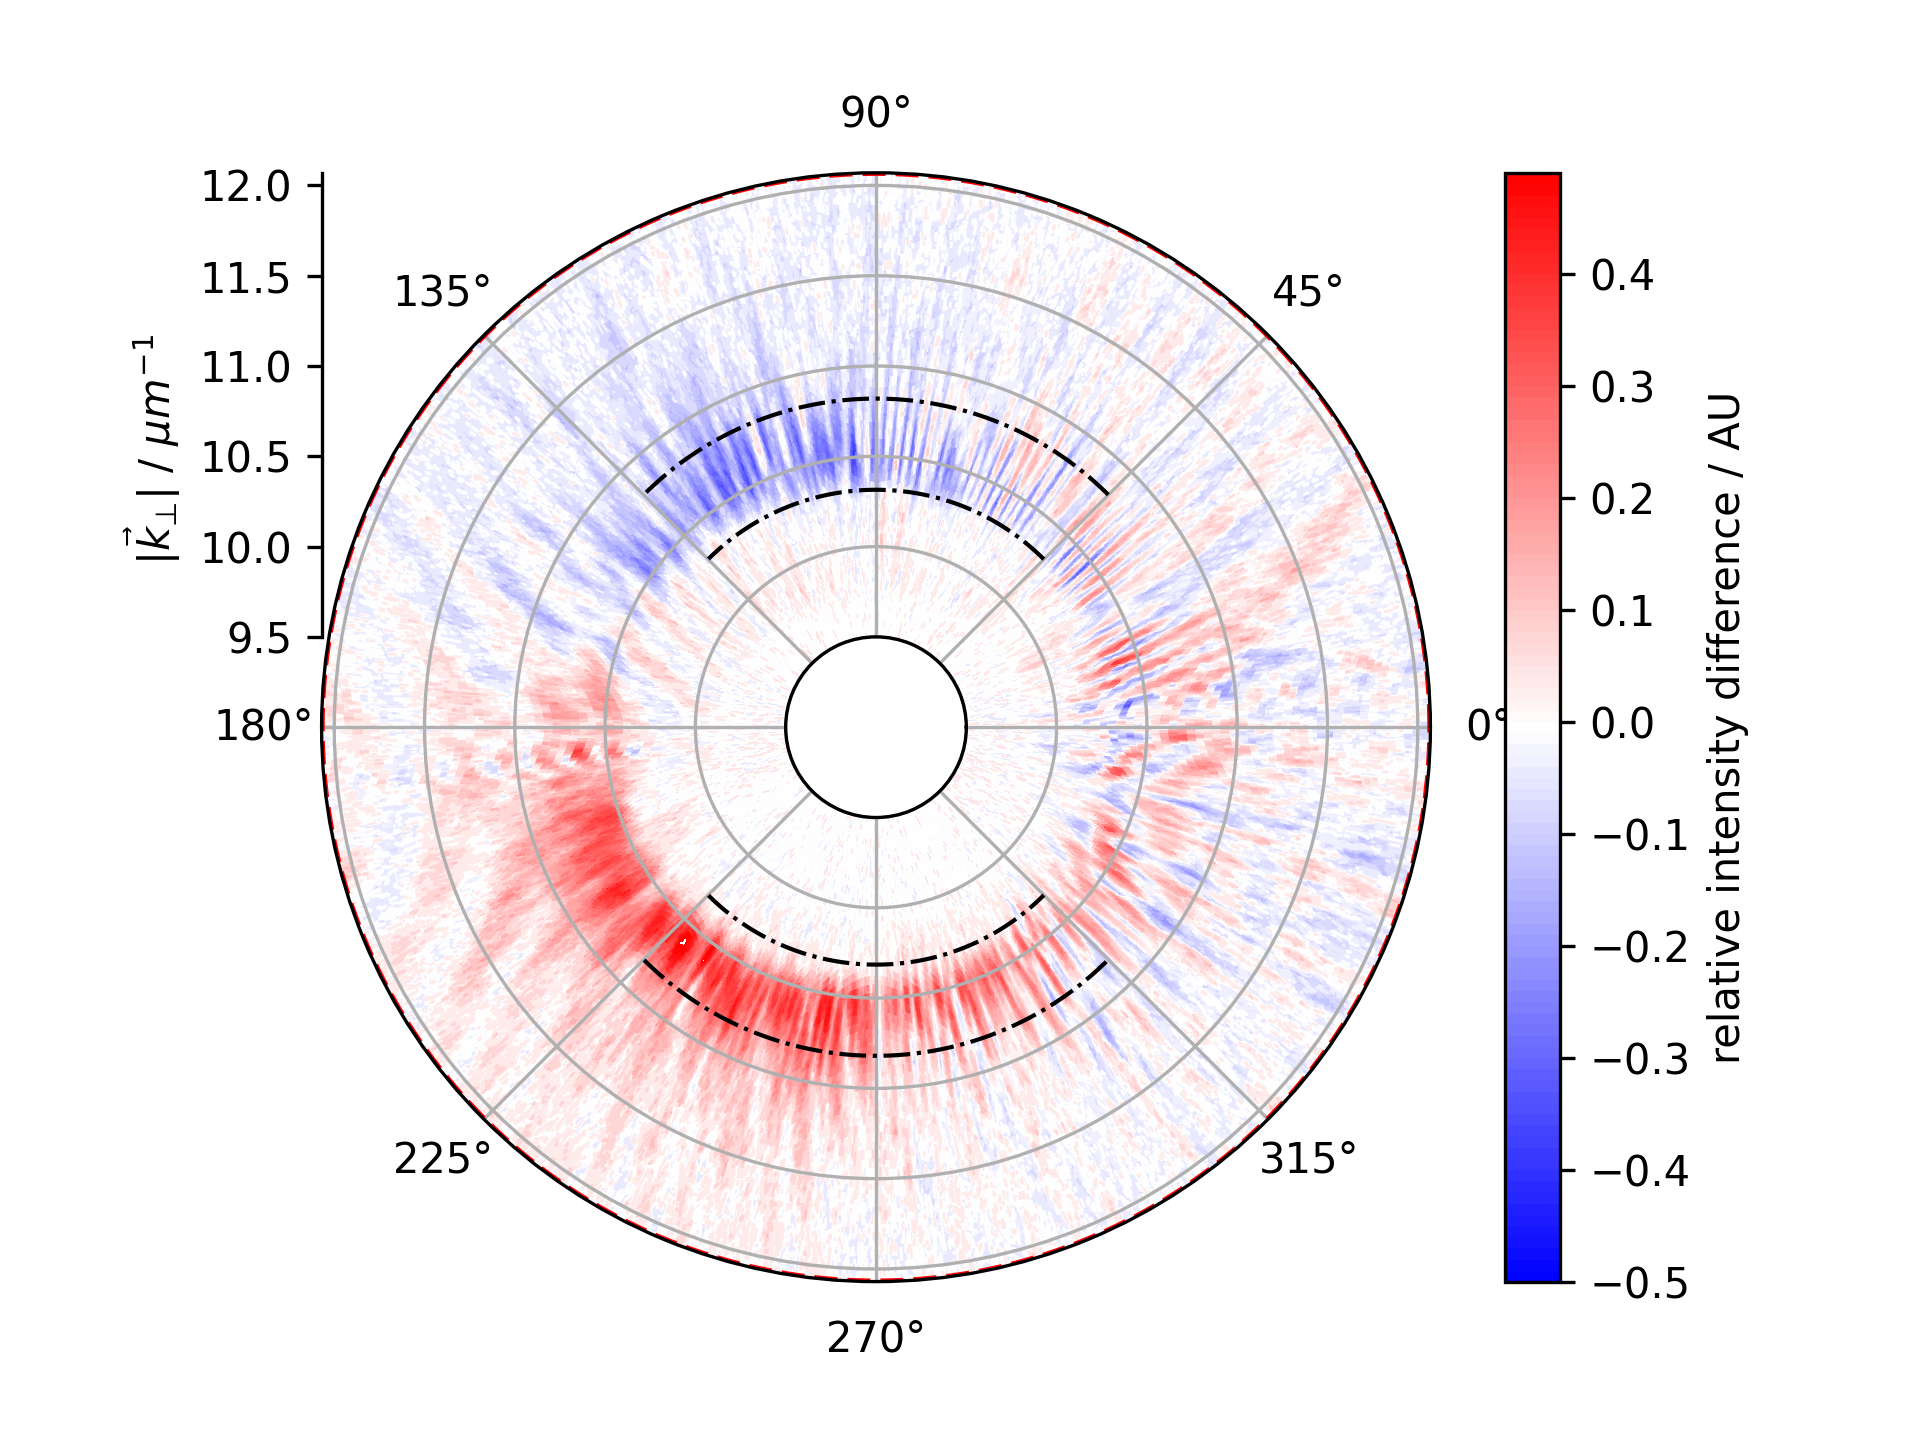
\includegraphics[width=\textwidth]{figures/spin_hall/diff_mid.png}
				\caption{$D_k\left(|\vec{k}_\perp|, \Phi\right)$}
				\label{fig:diff_mid}
			\end{subfigure}
			\hfill
			\begin{subfigure}[b]{0.49\textwidth}
				\centering
				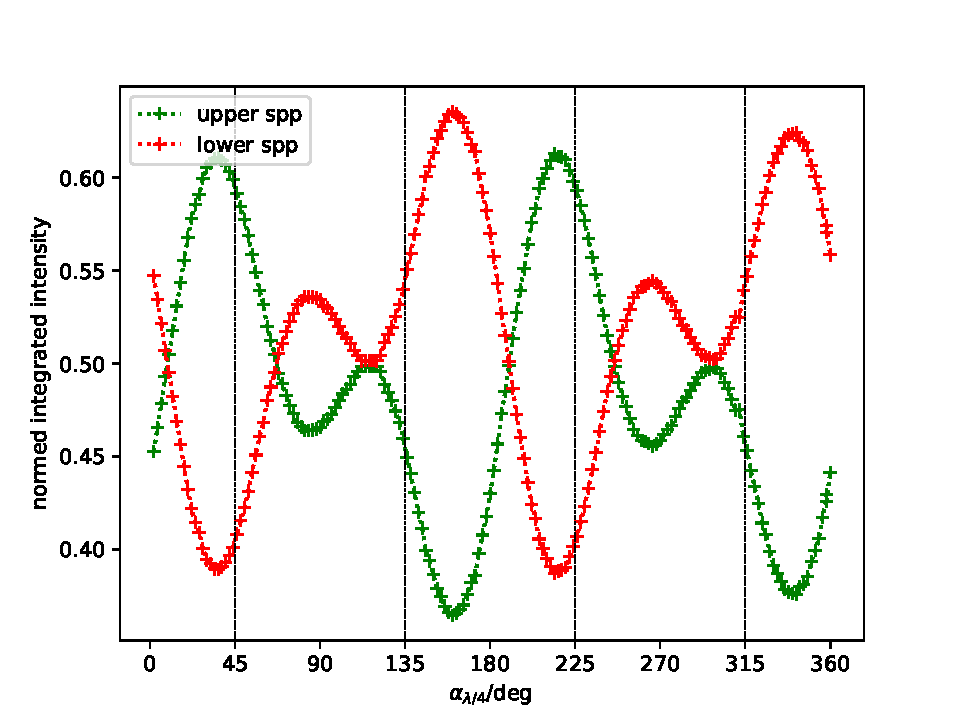
\includegraphics[width=\textwidth]{figures/spin_hall/intensity_mid.pdf}
				\caption{$\phi_\mathrm{min} =45^\circ, \phi_\mathrm{max}=135^\circ$}
				\label{fig:intensity_mid}
			\end{subfigure}
			
			\begin{subfigure}[b]{0.5\textwidth}
				\centering
				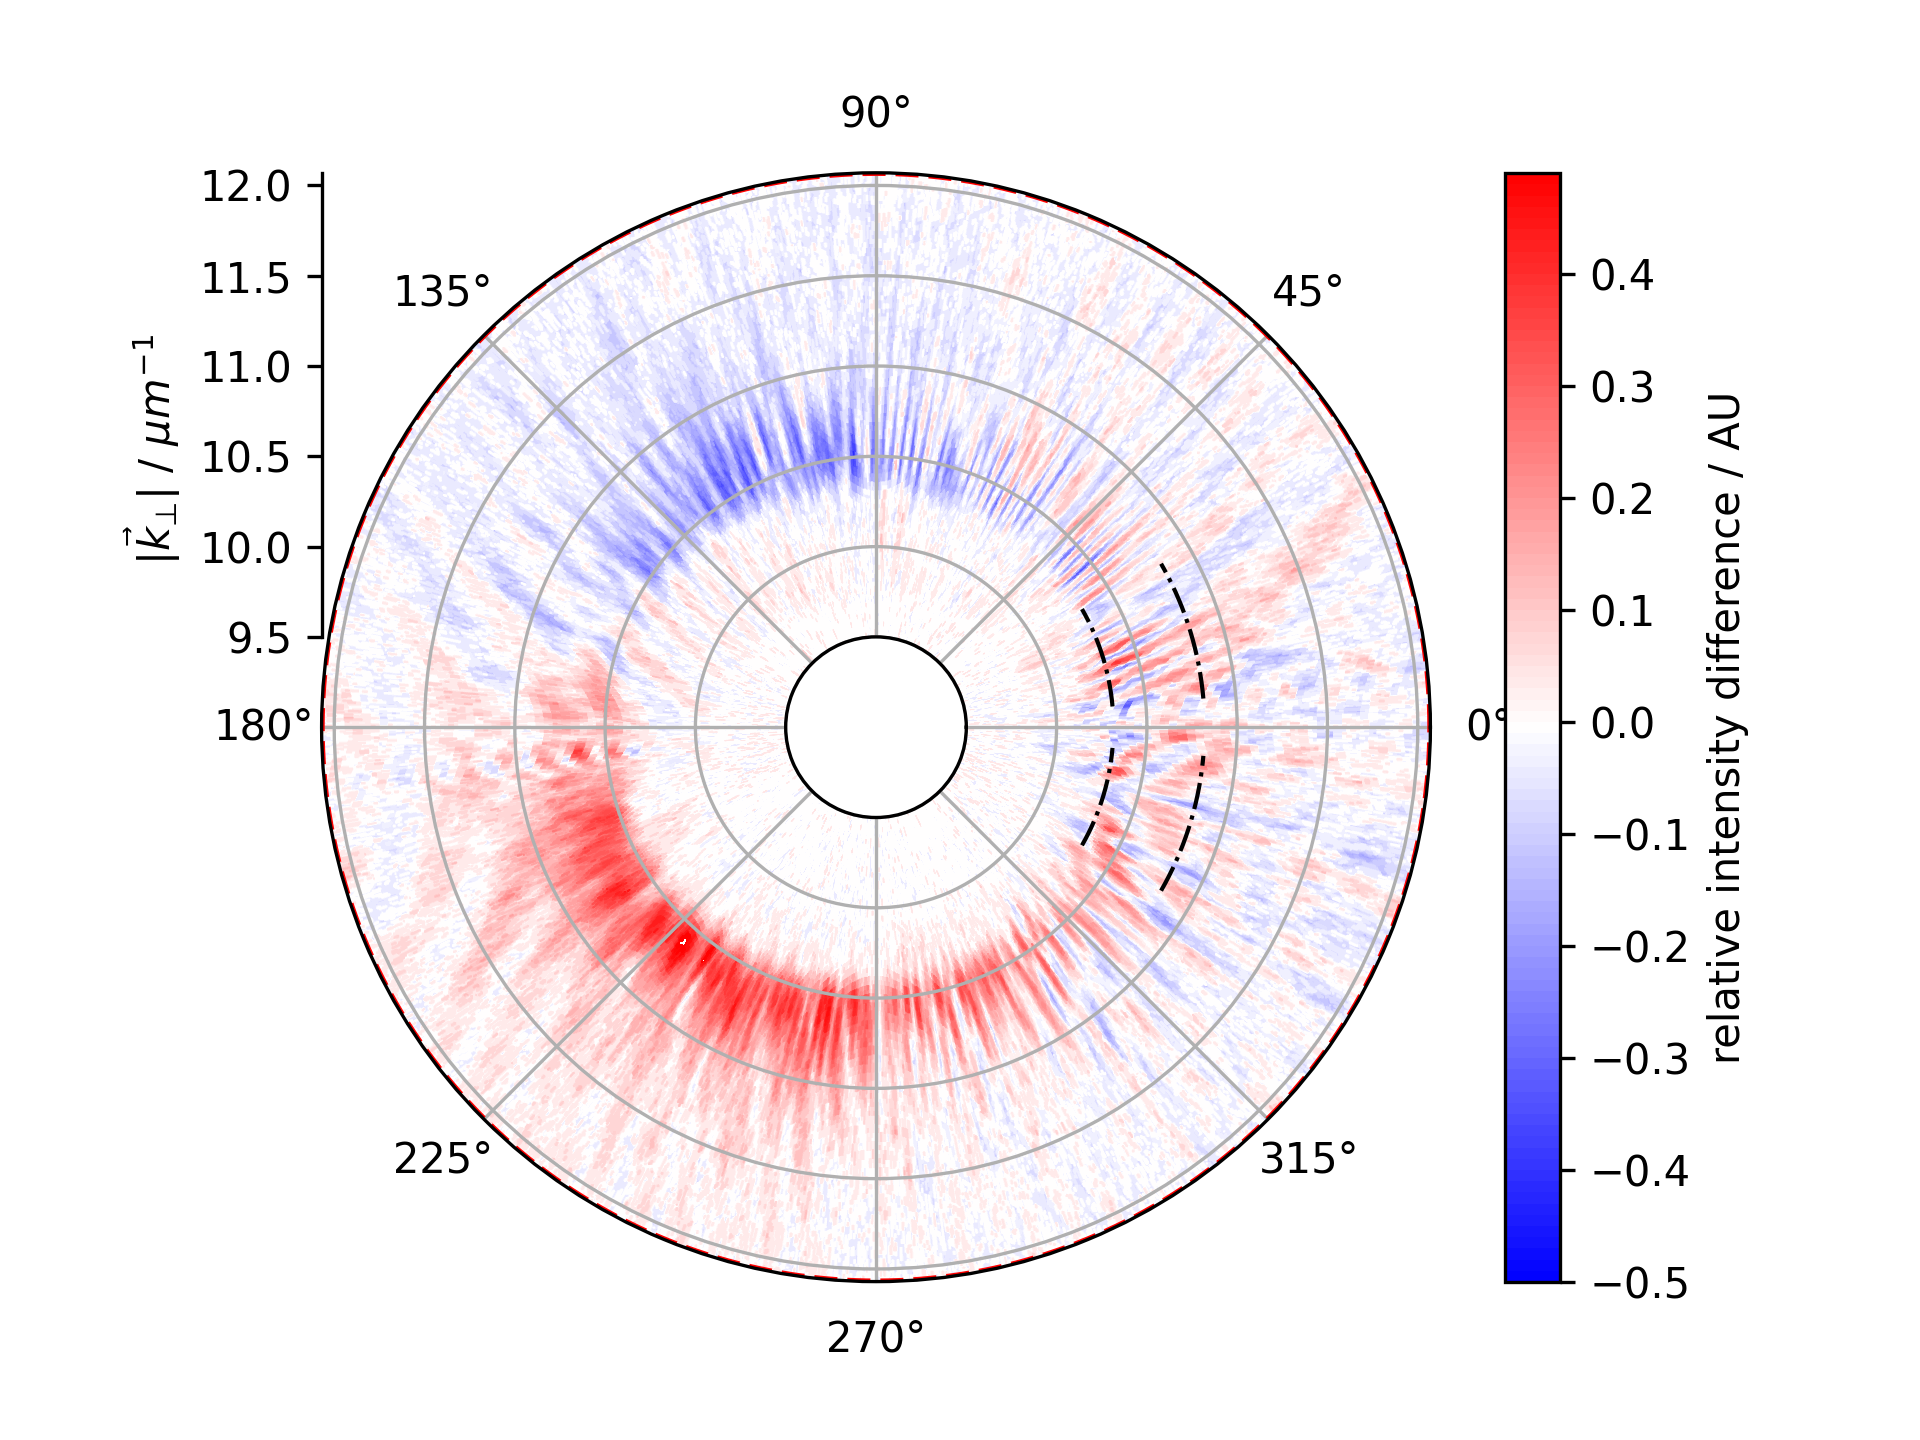
\includegraphics[width=\textwidth]{figures/spin_hall/diff_forw.png}
				\caption{$D_k\left(|\vec{k}_\perp|, \Phi\right)$}
				\label{fig:diff_front}
			\end{subfigure}
			\hfill
			\begin{subfigure}[b]{0.49\textwidth}
				\centering
				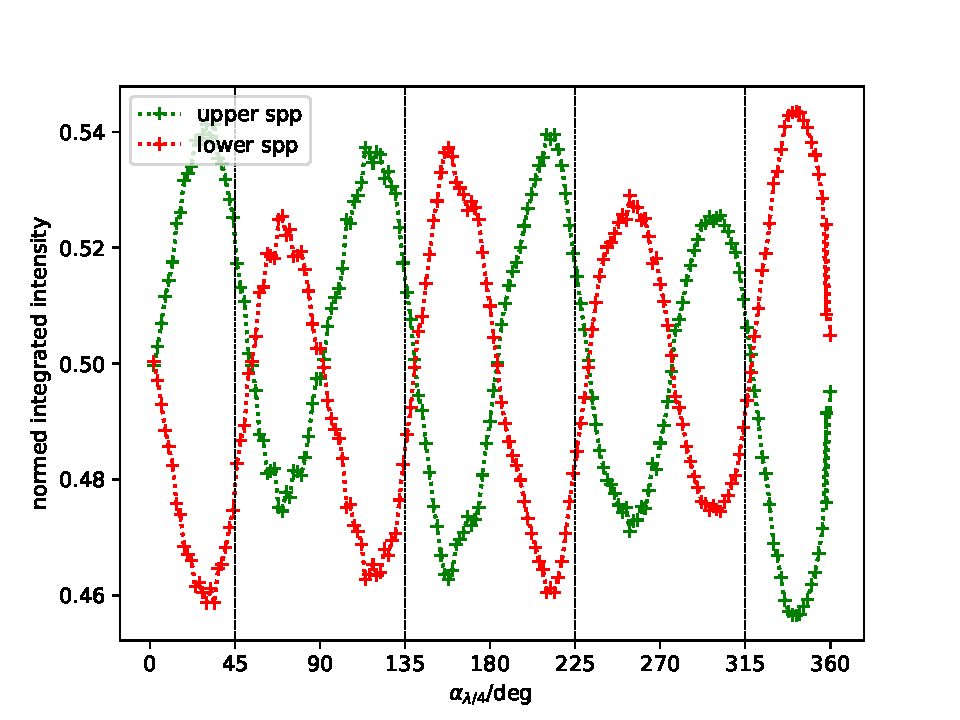
\includegraphics[width=\textwidth]{figures/spin_hall/intensity_forw.pdf}
				\caption{$\phi_\mathrm{min} =5^\circ, \phi_\mathrm{max}=30^\circ$}
				\label{fig:intensity_front}
			\end{subfigure}
			\caption[Differenz- und Integrationsdaten PSHE Impulsraum]{Die Abbildungen \subref{fig:diff_back}, \subref{fig:diff_mid}, \subref{fig:diff_front} zeigen die nach \eqref{eq:diff_measure_momentum} berechnete Differenz der Intensitäten im Impulsraum zwischen links- bzw. rechts-zirkular polarisierter Anregungsstrahlung. Diese Abbildungen unterscheiden sich nur durch die markierten Integrationsbereiche. Die Abbildungen \subref{fig:intensity_back}, \subref{fig:intensity_mid}, \subref{fig:intensity_front} zeigen jeweils die mit \eqref{eq:relative_power_momentum} über die zugehörigen markierten Bereiche integrierte Intensität normiert auf die Summe der Intensitäten beider Bereiche in Abhängigkeit der Orientierung des $\lambda/4$-Plättchens, also $P_{k, \mathrm{relativ}, \mathrm{Oben}}(\alpha_{\lambda/4})$ und $P_{k, \mathrm{relativ}, \mathrm{Unten}}(\alpha_{\lambda/4})$. Die vertikalen Linien markieren dabei die Orientierung des $\lambda/4$-Plättchens $\alpha_{\lambda/4}$, bei denen zirkulare Polarisation auftritt.}	
			\label{fig:spin_hall_measure}	
		\end{figure}
		\subparagraph{Analyse}
		\begin{itemize}
			\item In Rückwärtsrichtung (Abbildungen \ref{fig:diff_back} u. \ref{fig:intensity_back}) konnte der erwartete Effekt beobachtet werden. Bei zirkularer Polarisation ($\alpha_{\lambda/4} \in \{45^\circ, 135^\circ, 225^\circ, 315^\circ\}$) ist jeweils die maximale Asymmetrie in Bezug auf die Einfallsebene zu erkennen. Diese Asymmetrie wechselt beim Wechsel des Drehsinns der zirkularen Polarisation wie erwartet ihre Orientierung. Das beobachtete maximale Kontrastverhältnis ist hierbei $\eta = 1.6:1$. Dieses Kontrastverhältnis ist verglichen mit dem in \cite{OConnor.2014} beobachteten Kontrast von $\eta =7:1$ gering.  Die dort verwendete Nanostruktur war allerdings eine  $60\,\mathrm{nm}$ große Goldkugel, die mit der \textit{drop and cast} Methode auf der Goldoberfläche platziert worden ist. In der vorliegenden Arbeit wurde eine einfache Defektstelle auf dem Goldfilm für die Anregung verwendet. Die detaillierte Struktur dieses Defektes ist unbekannt und kann das Kontrastverhältnis beeinflussen.  Bei linearer Polarisation ($\alpha_{\lambda/4} \in \{0^\circ, 90^\circ, 180^\circ, 270^\circ\}$) verschwindet die Asymmetrie bis auf einen kleinen Rest, der vermutlich durch eine intrinsische Asymmetrie der Anregungsstruktur verursacht wird. Durch diese intrinsische Asymmetrie lässt sich auch erklären, dass das Kontrastverhältnis zwischen $135^\circ$ und $ 315^\circ$ jeweils etwas geringer ist als zwischen $45^\circ$ und $225^\circ$.
			Die intrinsische Asymmetrie der Struktur addiert sich auf die Asymmetrie, die durch den Spin-Hall-Effekt verursacht wird, und erhöht bzw. verringert diese im Wechsel.
			\item In Vorwärtsrichtung (Abbildungen \ref{fig:diff_front} u. \ref{fig:intensity_front}) konnte nicht der erwartete Effekt beobachtet werden. Hier tritt die maximale Asymmetrie jeweils bei elliptischer Polarisation auf und verschwindet bei zirkularer Polarisation. Bei linearer Polarisation verschwindet die Asymmetrie ebenfalls. Insgesamt zeigt der Verlauf die doppelte Frequenz der erwarteten Asymmetrie-Modulation. Daher ist das Signal auch symmetrisch bezüglich des Drehsinns der Polarisation. Für dieses Phänomen wurde im Rahmen dieser Arbeit keine endgültige Erklärung gefunden.
			
			Eine möglicher Erklärungsansatz ist die unbekannte Detailstruktur des Defektes. In den theoretischen Überlegungen ist von einem idealen Dipol ausgegangen worden. Wenn die Multipolentwicklung des polarisierten Defektes noch höhere, von Null verschiedene Terme aufweist, könnten weitere unbekannte Effekte auftreten. Dass durch kompliziertere Strukturen weitere nicht-triviale Effekte auftreten können, kann man auch in den Messungen (Abbildung \ref{fig:RF_measure_int}) aus \cite{RodriguezFortuno.2013} erkennen. Dort wurde der PSHE unter anderem an einer Gitterstruktur beobachtet. Die Messung an der Gitterstruktur zeigt auch eine gewisse Überlagerung von Signalen unterschiedlicher Frequenz. So ist dort bei ca. $10^\circ$ ein weiteres Maximum der \textit{left SPP intensity} zu erkennen, das durch die einfachen Modelle des Spin-Hall-Effektes nicht zu erklären ist. Diese Messungen bestätigen die Vermutung, dass kompliziertere Strukturen sich in nicht-trivialer Weise auf das Intensitätsbild auswirken. Eine andere Erklärung könnte darin bestehen, dass - anders als in der Simulation angenommen - kein ideal streifender Einfall vorlag, sondern die SPP  nur unter einem Einfallswinkel von $\alpha = 60^\circ$ zur Oberflächennormale angeregt wurden.  Auch diese andere Orientierung des Dipols könnte einen Effekt auf die Intensitätsverteilung in Abhängigkeit von der Polarisation haben.
			
			Bei genauerer Betrachtung des Differenzbildes zwischen links- und rechts-zirkularer Polarisation (Abbildung \ref{fig:diff_front}) fällt außerdem auf, dass das Differenzbild in Vorwärtsrichtung eine feine Struktur aufweist. Diese Struktur könnte durch Interferenzeffekte verursacht werden und gibt ebenfalls einen Hinweis auf die unbekannte Detailstruktur des Defektes.
			
			\item Senkrecht zur Einfallsebene (Abbildungen  \ref{fig:diff_mid} u. \ref{fig:intensity_mid}) wurde eine Überlagerung aus den oben beschriebenen Periodizitäten beobachtet. Diese Überlagerung führt dazu, dass das Signal des PSHE nicht mehr eindeutig zu identifizieren ist. Das überlagerte Signal zeigt Ähnlichkeit mit den in \cite{RodriguezFortuno.2013} durchgeführten Messungen an einer Gitterstruktur. Dort ist ebenfalls ein weiteres lokales Minimum der beiden Intensitäten bei linearer Polarisation zu beobachten (Vergleiche $\alpha_{\lambda/4}= 90$ aus Abbildung \ref{fig:intensity_mid} mit $\alpha_{\lambda/4}= 0$ aus Abbildung \ref{fig:RF_measure_int}). Die Darstellung in \ref{fig:RF_measure_int} zeigt jedoch absolute Intensitäten und keine relativen Intensitäten.
		\end{itemize}	
	
	\FloatBarrier
	\subsubsection{Polare Intensität und polare Intensitätsdifferenz}	
		Da für die unterschiedlichen Orientierungen des Integrationsbereichs qualitativ unterschiedliche Verhaltensweisen der Asymmetrie zwischen oberem und unterem SPP beobachtet worden sind, ist es sinnvoll, noch eine weiter Darstellungsart einzuführen:		
		
		 In Abbildung \ref{fig:angular_int_fp} wurde die über den Radius integrierte polarwinkelabhängige Intensitätsverteilung im Ortsbild bei einer Orientierung des $\lambda / 4$-Plättchens von $\alpha_{\lambda/4} = 45^\circ$ und  $\alpha_{\lambda/4} = 135^\circ$ dargestellt (also links- und rechts-zirkulare Polarisation). Um aus diesen Daten die polarwinkelabhängige Asymmetrie zwischen links- und rechts-polarisierter Anregungsstrahlung zu gewinnen, wurde aus den beiden Intensitäten die relative Differenz gebildet. Diese relative Differenz ist in Abbildung \ref{fig:angular_int_diff_fp} dargestellt.
		\paragraph{Ortsraum}
		\begin{align}
			\label{eq:integration_angular_int}
			P_r(\phi, \alpha_{\lambda/4}) &= \int_{0}^{r_\mathrm{max}}r\,\mathrm{d}r I_r(r, \phi, \alpha_{\lambda /4}) \\
			D_r(\phi) &= \dfrac{P_r(\phi, \alpha_{\lambda/4} = 45^\circ) - P_r(\phi, \alpha_{\lambda/4} = 135^\circ)}{P_r(\phi, \alpha_{\lambda/4} = 45^\circ) + P_r(\phi, \alpha_{\lambda/4} = 135^\circ)}
		\end{align}
		\begin{figure}		
			\begin{subfigure}[b]{0.5\textwidth}
				\centering
				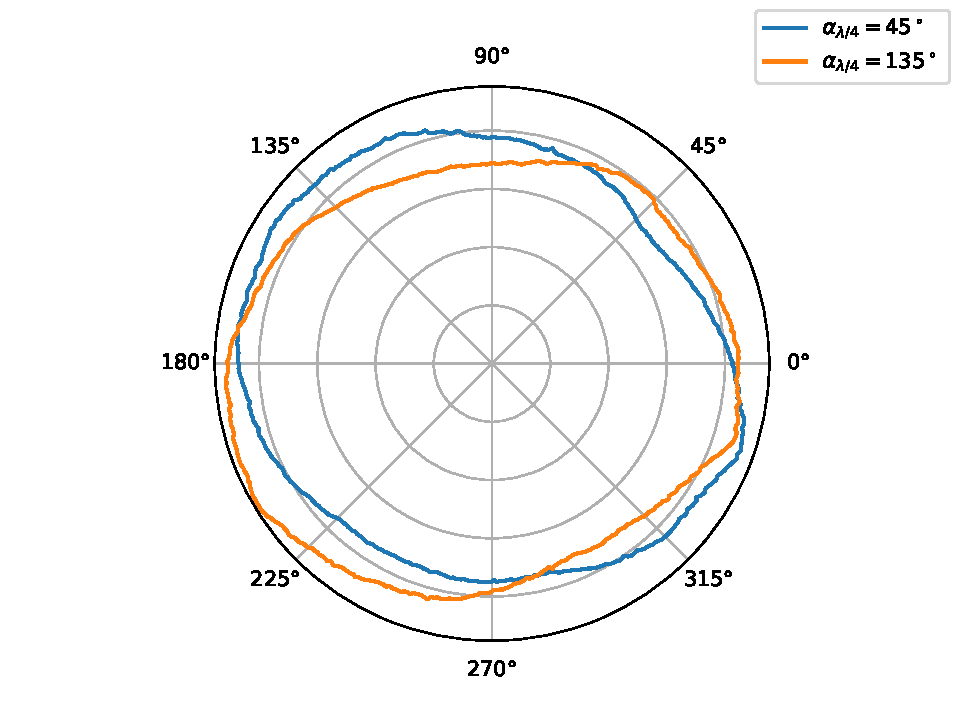
\includegraphics[width=\textwidth]{figures/spin_hall/fp_angular_distribution_45_135.pdf}
				\caption{Winkelabhängige Intensitätsverteilung}
				\label{fig:angular_int_fp}
			\end{subfigure}
			\hfill
			\begin{subfigure}[b]{0.49\textwidth}
				\centering
				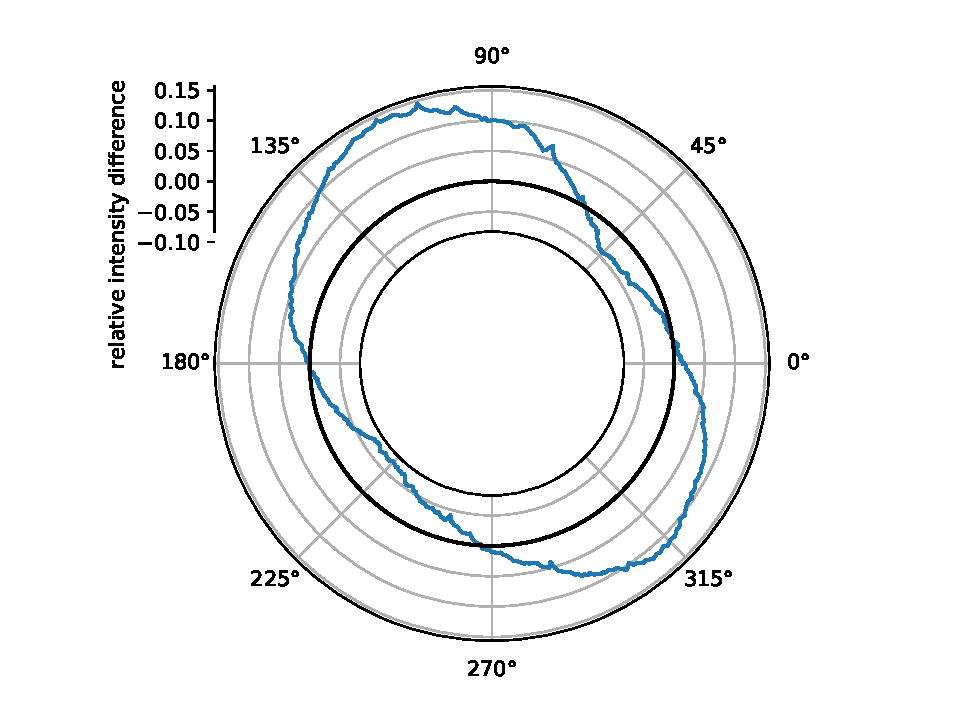
\includegraphics[width=\textwidth]{figures/spin_hall/fp_angular_distribution_diff_45_135.pdf}
				\caption{Winkelabhängige Intensitätsdifferenz}
				\label{fig:angular_int_diff_fp}
			\end{subfigure}
			\caption[Polarwinkel Auswertung Ortsraum]{Abbildung \subref{fig:angular_int_fp} zeigt die polar-winkelabhängige Intensitätsverteilung der Leckstrahlung eines an einem Punktdefekt angeregten SPP im Ortsraum bei links- und rechts-zirkular polarisierter Anregungsstrahlung. Abbildung \subref{fig:angular_int_diff_fp} zeigt die relative Differenz zwischen diesen beiden Intensitätsverteilungen. Die $0$-Linie wurde in der Differenzdarstellung durch einen zum Ursprung konzentrischen Kreisring markiert. Für die Darstellung wurde ein Polarkoordinatensystem gewählt, um den Bezug zu den Abbildungen \ref{fig:angular_int_diff_fp} besser herzustellen. Hierbei ist zu beachten, dass die von der Kurve eingeschlossenen Flächen nicht mehr der über einen Winkelbereich integrierten Intensitätsdifferenz entsprechen, da die Kurve durch die Darstellung in Polarkoordinaten verzerrt wird.}
			\label{fig:angular_dist_fp}
		\end{figure}
	
		\FloatBarrier
		\paragraph{Impulsraum}
		Diese Darstellung lässt sich analog auch für den Impulsraum einführen. Um dabei jeweils nur das plasmonische Signal und nicht das Hintergrundsignal darzustellen, wurde die Integration wieder nur von  $k_\mathrm{min}$ bis $k_\mathrm{max}$ durchgeführt.
		\begin{align}
			P_k(\phi, \alpha_{\lambda/4}) &= \int_{k_\mathrm{min}}^{k_\mathrm{max}}k\,\mathrm{d}k I_k(k, \phi, \alpha_{\lambda /4}) \\
			D_k(\phi) &= \dfrac{P_k(\phi, \alpha_{\lambda/4} = 45^\circ) - P_k(\phi, \alpha_{\lambda/4} = 135^\circ)}{P_k(\phi, \alpha_{\lambda/4} = 45^\circ) + P_k(\phi, \alpha_{\lambda/4} = 135^\circ)}
		\end{align}
		\begin{figure}		
			\begin{subfigure}[b]{0.5\textwidth}
				\centering
				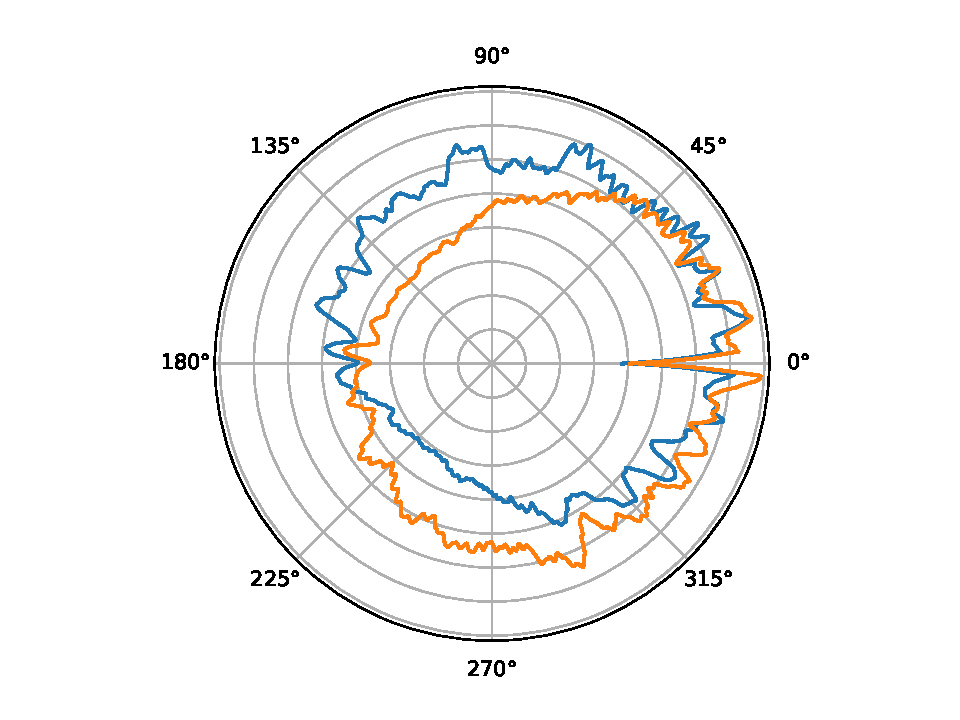
\includegraphics[width=\textwidth]{figures/spin_hall/bfp_angular_distribution_45_135.pdf}
				\caption{Winkelabhängige Intensitätsverteilung}
				\label{fig:angular_int_bfp}
			\end{subfigure}
			\hfill
			\begin{subfigure}[b]{0.49\textwidth}
				\centering
				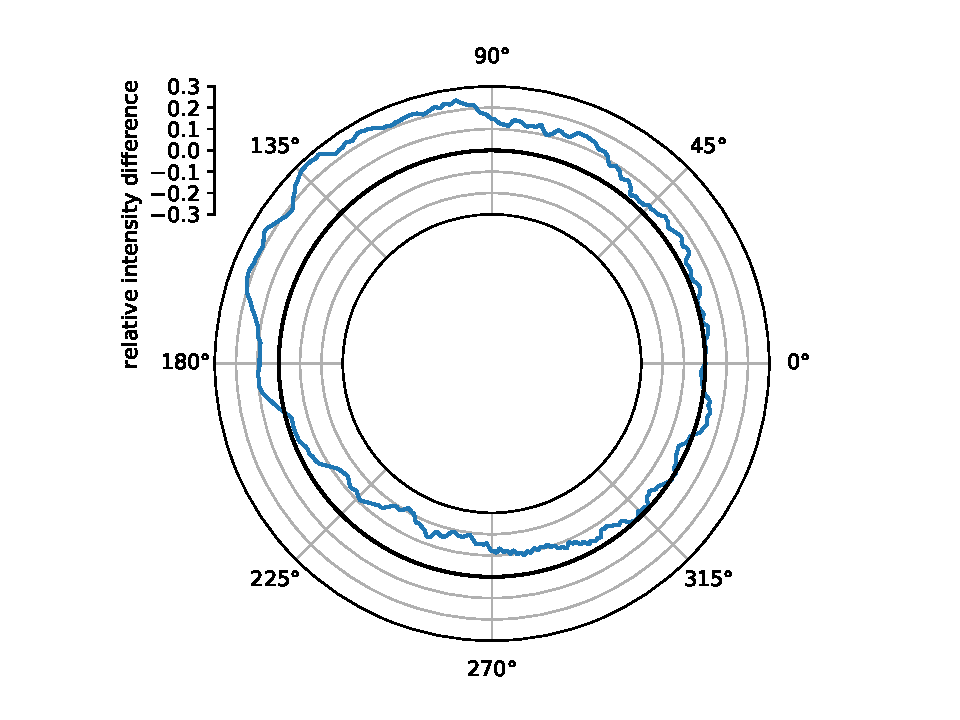
\includegraphics[width=\textwidth]{figures/spin_hall/bfp_angular_distribution_diff_45_135.pdf}
				\caption{Winkelabhängige Intensitätsdifferenz}
				\label{fig:angular_int_diff_bfp}
			\end{subfigure}
			\caption[Polarwinkel Auswertung Impulsraum]{Abbildung \subref{fig:angular_int_fp} zeigt die polar-winkelabhängige Intensitätsverteilung der Leckstrahlung eines an einem Punktdefekt angeregten SPP im Ortsraum bei links- und rechts-zirkular polarisierter Anregungsstrahlung. Abbildung \subref{fig:angular_int_diff_fp} zeigt die relative Differenz zwischen diesen beiden Intensitätsverteilungen. Die $0$-Linie wurde in der Differenzdarstellung durch einen zum Ursprung konzentrischen Kreisring markiert. Für die Darstellung wurde ein Polarkoordinatensystem gewählt, um den Bezug zu den Abbildungen \ref{fig:angular_int_diff_fp} besser herzustellen. Hierbei ist zu beachten, dass die von der Kurve eingeschlossenen Flächen nicht mehr der über einen Winkelbereich integrierten Intensitätsdifferenz entsprechen, da die Kurve durch die Darstellung in Polarkoordinaten verzerrt wird.}
			\label{fig:angular_dist_bfp}
		\end{figure}
		\paragraph{Analyse}
		In den polaren Intensitätsdaten kann man das oben beschriebene Asymmetrieverhalten noch einmal deutlicher erkennen. In der polarwinkelabhängigen Intensitätsverteilung des Ortsbildes (Abbildung \ref{fig:angular_int_fp}) ist in Vorwärtsrichtung eine Asymmetrie mit umgekehrtem Vorzeichen zur Asymmetrie in Rückwärtsrichtung zu erkennen. Diese wechselnde Asymmetrie ist in der polarwinkelabhängigen Intensitätsverteilung des Impulsraumes (Abbildung \ref{fig:angular_int_bfp}) nicht zu beobachten. Hier tritt in dem Bereich $\phi \in [45^\circ, 315^\circ]$ eine gleichbleibende Asymmetrie auf. In Vorwärtsrichtung ist keine nennenswerte Asymmetrie zu beobachten. Diese Diskrepanz zwischen der winkelabhängigen Orts- und Impulsbilddarstellung ist dadurch zu erklären, dass in der Intensitätsverteilung im Ortsraum nicht zwischen dem plasmonischen und dem Hintergrundsignal unterschieden werden kann. Daher wird die Integration im Ortsraum \eqref{eq:integration_angular_int} zwangsweise auch über das Hintergrundsignal ausgeführt. Bei der Integration im Impulsraum wird durch die radialen Integrationsgrenzen $k_\mathrm{min}$ und $k_\mathrm{max}$ hauptsächlich das plasmonische Signal selektiert. Eine Diskrepanz zwischen Orts- und Impulsraum tritt außerdem auf, falls noch ein weiterer Defekt an der Anregung beteiligt ist. Wenn ein weiteres Anregungszentrum in der optischen Abbildung liegt, entspricht die Richtung zwischen Ursprung und einem Punkt im Ortsraum nicht mehr der Ausbreitungsrichtung des SPP. In den Rohdaten des Ortsbildes (Abbildung \ref{fig:raw_fp_45}) ist zu erahnen, dass rechts neben dem Bildausschnitt ein weiteres Anregungszentrum liegt.	\begin{figure}
			\label{fig:RF_measure}
			\centering
			\begin{subfigure}[b]{0.5\textwidth}
				\centering
				\includegraphics[width=\textwidth]{figures/RF_SM_Slits.pdf}
				\caption{Struktur}
				\label{fig:RF_measure_slits}
			\end{subfigure}
			\hfill
			\begin{subfigure}[b]{0.49\textwidth}
				\centering
				\includegraphics[width=\textwidth]{figures/RF_SM_Intensity.pdf}
				\caption{Intensitätsverteilung}
				\label{fig:RF_measure_int}
			\end{subfigure}
			\caption[Vergleichsmessung aus \cite{RodriguezFortuno.2013}]{Die Abbildung zeigt die Messungen aus \cite{RodriguezFortuno.2013}, die an einer Gitterstruktur durchgeführt wurden.}			
		\end{figure}
	\newpage
	\section{Zusammenfassung und Ausblick}
	In dieser Arbeit wurde erfolgreich ein bestehendes Leckstrahlmikroskop modifiziert und in einigen Details verbessert. Der Strahlgang des Lasers wurde so verändert, dass die Einkopplung des Lasers unter schrägem Einfall auf die Probe erfolgen konnte. Hierfür musste das Einkoppelobjektiv durch einen einfache Sammellinse ersetzt werden. Außerdem wurde ein Polarisationsfilter und eine $\lambda/4$-Platte zur Kontrolle der Polarisation des Lasers verbaut. Es wurden außerdem zahlreiche Optomechaniken ausgetauscht. Durch diese Modifikationen konnte am Ende dieser Arbeit tatsächlich der plasmonischen Spin-Hall-Effekt (PSHE) nachgewiesen werden. Der PSHE wurde besonders deutlich in Rückwärtsrichtung bezogen auf die Einfallsrichtung der anregenden Strahlung beobachtet. Hier konnte ein Kontrastverhältnis von $\eta = 1.6$ zwischen zwei Propagationsrichtungen beobachtet werden. In Vorwärtsrichtung hingegen sind die Beobachtungn nicht so deutlich ausgefallen. Um des Verhalten in Vorwärtsrichtung genauer zu untersuchen wäre eine Simulation mit Hilfe der Transfermatrixmethode und dem Raumfrequenzspektrum eines $3d$-Dipols notwendig. Eventuell könnten durch diese Simulationen weiter Effekte quantitativ verstanden werden. Außerdem könnte die unbekannte Detail-Struktur des Defektes durch gezielt hergestellte Anregungszentren als mögliche Fehlerquelle eliminiert werden. Des weiteren wäre es interessant, die Messung an einer größeren Zahl von Defekten durchzuführen, und dann durch Messstatistik Effekte die aufgrund einer Substruktur des Defektes entstehen von systematischen Effekten zu unterscheiden.
	
	\newpage
	\appendix
	\bibliography{bib}
	\newpage
	\section{Weitere Messdaten}
	\begin{figure}[h!]
		\label{fig:dirt_measure}
		\centering
		\begin{subfigure}[b]{0.5\textwidth}
			\centering
			\includegraphics[width=\textwidth]{figures/dirt_radial.pdf}
			\caption{Radial-Profil}
			\label{fig:dirt_radial}
		\end{subfigure}
		\hfill
		\begin{subfigure}[b]{0.49\textwidth}
			\centering
			\includegraphics[width=\textwidth]{figures/dirt_lorentz.pdf}
			\caption{Lorentz-Fit}
			\label{fig:dirt_lorentz}
		\end{subfigure}
	
		\begin{subfigure}[b]{0.7\textwidth}
		\centering
		\includegraphics[width=\textwidth]{figures/dirt_polar.png}
		\caption{Intensitätsverteilung}
		\label{fig:dirt_polar}
		\end{subfigure}
		\caption[Messung an kontaminierter Probe]{Die Abbildung zeigt die BFP bei der Messung an einer mit Öl kontaminierten Probe unter senkrechtem Laser-Einfall. Der Wellenvektor wurde hier mit Hilfe eines Lorentz-Fits auf $k_\mathrm{SPP} = (11.0 + 0.4i)\,\mathrm{\mu m}^{-1}$ bestimmt. Die Dämpfung ist hier also signifikant größer als bei den Messungen an nicht kontaminierten Proben.}			
	\end{figure}

	\begin{figure}[h!]
	\label{fig:measure_linear_polarisation}
	
	\begin{subfigure}[b]{0.49\textwidth}
		\centering
		\includegraphics[width=\textwidth]{figures/fp/fp_0.png}
		\caption{$\alpha_{\lambda/4} = 0^\circ$}
	\end{subfigure}
	\begin{subfigure}[b]{0.5\textwidth}
		\centering
		\includegraphics[width=\textwidth]{figures/spin_hall/polar/polar_0.png}
		\caption{$\alpha_{\lambda/4} = 0^\circ$}
	\end{subfigure}
	\hfill
	\begin{subfigure}[b]{0.49\textwidth}
		\centering
		\includegraphics[width=\textwidth]{figures/fp/fp_90.png}
		\caption{$\alpha_{\lambda/4} = 90^\circ$}
	\end{subfigure}
	\begin{subfigure}[b]{0.5\textwidth}
		\centering
		\includegraphics[width=\textwidth]{figures/spin_hall/polar/polar_90.png}
		\caption{$\alpha_{\lambda/4} = 90^\circ$}
	\end{subfigure}

	\caption[Orts- und Impulsraum Rohdaten bei linearer Polarisation]{Die Abbildung zeigt den Orts und den Impulsraum bei der Messung an einem Punktdefekt unter streifenden Laser-Einfall mit linearer Polarisation.}			
\end{figure}
	\newpage
	\section{Technische Zeichnungen}
	\begin{figure}[h!]
		\centering
		\includegraphics[width=1\linewidth]{figures/tube_lense_tz}
		\caption{Technische Zeichnung der Tubus-Linse}
		\label{fig:tubelensetz}
	\end{figure}
	
	\begin{sidewaysfigure}[h!]
		\includegraphics[width=\textwidth]{figures/Technische_Zeichnung_Probenhalter.pdf}
		\caption{Technische Zeichnung Probenhalter}
		\label{fig:tz_probenhalter}
	\end{sidewaysfigure}
	\begin{sidewaysfigure}[h!]
		\includegraphics[width=\textwidth]{figures/Probenblech.pdf}
		\caption{Technische Zeichnung Probenblech}
		\label{fig:tz_probenblech}
	\end{sidewaysfigure}
	\begin{sidewaysfigure}[h!]
		\includegraphics[width=\textwidth]{figures/LinsenAdapter.pdf}
		\caption{Technische Zeichnung Linsen-Adapter}
		\label{fig:tz_adapter}
	\end{sidewaysfigure}
	\begin{sidewaysfigure}[h!]
		\includegraphics[width=\textwidth]{figures/4f_system.pdf}
		\caption{Technische Zeichnung Cage-System}
		\label{fig:tz_cage_system}
	\end{sidewaysfigure}
	\newpage
	\section{Liste der verwendeten Komponenten}
	\begin{table}[h!]
		\centering	
		\begin{tabular}{|c|c|c|}
			\hline
			\textbf{Bauteil}         & \textbf{Typ}                   & \textbf{Hersteller}                    \\
			\hline
			\hline
			Helium-Neon-Laser        & HNL210L-EC                     & \textit{Thorlabs}                      \\
			ND Filter                & NDL-25C-2                      & \textit{Thorlabs}                      \\
			$\lambda/4$-Plättchen    & WPMQ05M-633                    & \textit{Thorlabs}                      \\
			Polarisationsfilter      & -        					  & \textit{Newport}                       \\
			Hintergrund LED          & -          					  & -                  					   \\
			Blenden                  & -          					  & -                  					   \\
			Spiegel                  & -          					  & -                  					   \\
			Kollimatorlinse          & Lens Asphere Ach 25x40Vis 0 TS & \textit{Edmund Optics}                 \\
			Immersionsobjektiv       & 100-fach/1.25 N-Achroplan      & \textit{Carl Zeiss}                    \\
			Immersionsöl             & 518N, n=1.518                  & \textit{Carl Zeiss}                    \\
			Tubuslinse               & 452149-0000-000                & \textit{Carl Zeiss}                    \\
			2x Linsen                & LA1417-A-ML, f = 150 mm        & \textit{Thorlabs}                      \\
			1x Linsen                & LA1417-A-ML, f = 75 mm         & \textit{Thorlabs}                      \\
			2x Lineartisch           & 2000551						  &\textit{Thorlabs} 					   \\
			Kristallhalter           & LP-1A (XYZ) Series             & \textit{Newport}                       \\
			Objektiv-Adapter         & LPMH-1                         & \textit{Newport}                       \\
			3-Achsen-Bühne           & TSD                            & \textit{OptoSigma}                     \\
			2-Achsen-Bühne           & TSD                            & \textit{OptoSigma}                     \\
			Filter-Halter            & FH2                            & \textit{Thorlabs}                      \\
			Einkoppellinse           & LA-1805                        & \textit{Thorlabs}                      \\
			Linsenhalter             & M-LH-1A                        & \textit{Newport}                       \\
			Cage Plate               & LCP08/M                        & \textit{Thorlabs}                      \\
			Linsen Tubus Verbinder   & CMT2                           & \textit{Thorlabs}                      \\
			SM2, CMount Adapter      & SM2A54                         & \textit{Thorlabs}                      \\
			Justierbarer Linsentubus & SM2V05                         & \textit{Thorlabs}                      \\
			Magnet Cage-Plate        & LCP90F                         & \textit{Thorlabs}                      \\
			3x xy-Linsenhalter       & CXY2                           & \textit{Thorlabs}                      \\
			3x Cage-System-Halter    & LCP01B                         & \textit{Thorlabs}                      \\
			4x Cage-System-Stange    & ER8                            & \textit{Thorlabs}                      \\
			4x Cage-System-Stange    & ER24                           & \textit{Thorlabs}                      \\
			4x Stangenverbinder      & ERSCB                          & \textit{Thorlabs}                      \\
			CageSystem Justier Hilfe & LCPA1                          & \textit{Thorlabs}                      \\
			CMOS IP-Kamera 			 & Mako G307C					  &	\textit{Allied Vision}				   \\
			Probenhalter		     & Eigendesign                    & Werkstatt                              \\
			Probenblech              & Eigendesign                    & Werkstatt                              \\
			BeamBlock                & Eigendesign                    & Werkstatt                              \\
			Tubuslinsenhalter        & Eigendesign                    & Werkstatt                              \\
			\hline          
		\end{tabular}
		\caption{Liste der verwendeten Komponenten}
		\label{tab:components}
	\end{table}
\newpage
\section*{Erklärung der Urheberschaft}

Ich erkläre hiermit an Eides statt, dass ich die vorliegende Arbeit
ohne Hilfe Dritter und ohne Benutzung anderer als der angegebenen
Hilfsmittel angefertigt habe; die aus fremden Quellen direkt oder
indirekt übernommenen Gedanken sind als solche kenntlich gemacht. Die
Arbeit wurde bisher in gleicher oder ähnlicher Form in keiner anderen
Prüfungsbehörde vorgelegt und auch noch nicht veröffentlicht.

\vspace{4cm}

\hspace{2cm} Ort, Datum \hfill Unterschrift \hspace{2cm}
	
	
\end{document}
